%% LaTeX-Beamer template for KIT design
%% by Erik Burger, Christian Hammer
%% title picture by Klaus Krogmann
%%
%% version 2.1
%%
%% mostly compatible to KIT corporate design v2.0
%% http://intranet.kit.edu/gestaltungsrichtlinien.php
%%
%% Problems, bugs and comments to
%% burger@kit.edu
\documentclass[16pt,usenames,dvipsnames, notheorems]{beamer}

\usepackage{xcolor}
\usepackage{rotating}
\usepackage{mathtools}% Loads amsmath
\usepackage{adjustbox}
\usepackage{array}

\newcolumntype{R}[2]{%
	>{\adjustbox{angle=#1,lap=\width-(#2)}\bgroup}%
	l%
	<{\egroup}%
}
\newcommand*\rot{\multicolumn{1}{R{45}{0.5em}}}% no optional argument here, please!

\usepackage[symbol]{footmisc}

\usepackage[utf8]{inputenc}
\usepackage{animate}
\usepackage{subcaption}
\usepackage{caption}
\setbeamertemplate{caption}[numbered]
\setbeamertemplate{bibliography item}{\insertbiblabel}
\usepackage{graphicx}
\usepackage{grffile}
\usepackage{ragged2e}
\usepackage{url}

\usepackage[square,numbers]{natbib}

\usepackage{algorithm}
\usepackage{balance}
\usepackage[noend]{algpseudocode}

\usepackage{amsfonts}
\usepackage{booktabs}
\usepackage{siunitx}
\usepackage{threeparttable}
\usepackage{tabularx}

\usepackage{amssymb}
\usepackage{pifont}
\newcommand{\cmark}{\ding{51}}
\newcommand{\xmark}{\ding{55}}
\usepackage{tablefootnote}

\setbeamerfont{bibliography item}{size=\footnotesize}
\setbeamerfont{bibliography entry author}{size=\footnotesize}
\setbeamerfont{bibliography entry title}{size=\footnotesize}
\setbeamerfont{bibliography entry location}{size=\footnotesize}
\setbeamerfont{bibliography entry note}{size=\footnotesize}

\setbeamerfont{block title}{size=\scriptsize}
\captionsetup{font=scriptsize,labelfont=scriptsize}

\setbeamertemplate{theorem}[ams style]
\setbeamertemplate{theorems}[numbered]
\setbeamertemplate{definitions}[numbered]

% Done as in https://tex.stackexchange.com/questions/82415/beamer-different-numbering-for-theorems-examples-definition-and-lemma
\makeatletter
\ifbeamer@countsect
\newtheorem{theorem}{\translate{Theorem}}[section]
\else
\newtheorem{theorem}{\translate{Theorem}}
\fi
\newtheorem{corollary}{\translate{Corollary}}
\newtheorem{fact}{\translate{Fact}}
\newtheorem{lemma}{\translate{Lemma}}
\newtheorem{problem}{\translate{Problem}}
\newtheorem{solution}{\translate{Solution}}

\theoremstyle{definition}
\newtheorem{definition}{\translate{Definition}}
\newtheorem{definitions}{\translate{Definitions}}

\theoremstyle{example}
\newtheorem{example}{\translate{Example}}
\newtheorem{examples}{\translate{Examples}}

% Compatibility
\newtheorem{Beispiel}{Beispiel}
\newtheorem{Beispiele}{Beispiele}
\theoremstyle{plain}
\newtheorem{Loesung}{L\"osung}
\newtheorem{Satz}{Satz}
\newtheorem{Folgerung}{Folgerung}
\newtheorem{Fakt}{Fakt}
\newenvironment{Beweis}{\begin{proof}[Beweis.]}{\end{proof}}
\newenvironment{Lemma}{\begin{lemma}}{\end{lemma}}
\newenvironment{Proof}{\begin{proof}}{\end{proof}}
\newenvironment{Theorem}{\begin{theorem}}{\end{theorem}}
\newenvironment{Problem}{\begin{problem}}{\end{problem}}
\newenvironment{Corollary}{\begin{corollary}}{\end{corollary}}
\newenvironment{Example}{\begin{example}}{\end{example}}
\newenvironment{Examples}{\begin{examples}}{\end{examples}}
\newenvironment{Definition}{\begin{definition}}{\end{definition}}
\makeatother

%% SLIDE FORMAT
% use 'beamerthemekit' for standard 4:3 ratio
% for widescreen slides (16:9), use 'beamerthemekitwide'
\usepackage{templates/beamerthemekit}
% \usepackage{templates/beamerthemekitwide}

\usepackage{tikz}
\usetikzlibrary{calc}
\usetikzlibrary{patterns}

\usepackage{mathtools}
\usepackage{relsize}
%% TITLE PICTURE

% if a custom picture is to be used on the title page, copy it into the 'logos'
% directory, in the line below, replace 'mypicture' with the 
% filename (without extension) and uncomment the following line
% (picture proportions: 63 : 20 for standard, 169 : 40 for wide
% *.eps format if you use latex+dvips+ps2pdf, 
% *.jpg/*.png/*.pdf if you use pdflatex)
\titleimage{defense_cover}

%% TITLE LOGO
% for a custom logo on the front page, copy your file into the 'logos'
% directory, insert the filename in the line below and uncomment it
\titlelogo{blank}
% (*.eps format if you use latex+dvips+ps2pdf,
% *.jpg/*.png/*.pdf if you use pdflatex)

%% TikZ INTEGRATION
% use these packages for PCM symbols and UML classes
% \usepackage{templates/tikzkit}
% \usepackage{templates/tikzuml}
% the presentation starts here

\title[Estimating Dependency, Monitoring and Knowledge Discovery in HD-DS]{\large Estimating Dependency, Monitoring and Knowledge Discovery in High-Dimensional Data Streams}
\subtitle{Doctoral Defense}
\author{Edouard Fouché}

\institute{Advisor: Prof. Dr.-Ing. Klemens Böhm}

% Bibliography
%\usepackage[citestyle=alphabetic-verb,bibstyle=numeric,hyperref,backend=biber]{biblatex}
%\addbibresource{templates/example.bib}
%\bibhang1em
\setbeamerfont{bibliography item}{size=\footnotesize}
\setbeamerfont{bibliography entry author}{size=\footnotesize}
\setbeamerfont{bibliography entry title}{size=\footnotesize}
\setbeamerfont{bibliography entry location}{size=\footnotesize}
\setbeamerfont{bibliography entry note}{size=\footnotesize}

\definecolor{uiucblue}{RGB}{19,42,76}
\definecolor{uiucred}{RGB}{232,74,39}
\definecolor{kitgreen}{RGB}{43,135,115}

\definecolor{specialblue}{RGB}{49,75,108}
\definecolor{specialorange}{RGB}{246,128,40}
\RequirePackage{hyperref}
\begin{document}
% change the following line to "ngerman" for German style date and logos
\selectlanguage{english}

%title page
\begin{frame}
\titlepage
\end{frame}

% Good afternoon everyone and thank you for attending. Welcome to the defence of my dissertation "Estimating Dependency, Monitoring and Knowledge Discovery in High-Dimensional Data Streams". The presentation will last about 25 minutes, and I will take questions afterwards. Let's start with the motivations of my thesis: 
\section{Introduction}
\subsection{Motivations}

\begin{frame}{Motivations}

\textit{Data Mining} -- or \textit{Knowledge Discovery from Data (KDD)} -- is the process of extracting knowledge from massive data sets. 
\begin{itemize}
	\item Data Mining has massive impact on our daily lives. 
\end{itemize}
~\\
\pause
Modern tasks often involve data that: 
\begin{itemize}
	\item is \textit{high-dimensional} (many attributes)
	\pause
	\item comes as a \textit{stream} (continuously collected)
	\pause
	\item or both ! (high-dimensional + stream)
\end{itemize}
\begin{figure}
	\begin{subfigure}[c]{0.25\linewidth}
		\centering
		\begin{overprint}
			\onslide<1> 
\includegraphics[width=\linewidth]{figures/picture_biology_t.jpg}
			\onslide<2-> 
\includegraphics[width=\linewidth]{figures/picture_biology.jpg}
		\end{overprint}
		%\caption*{Biology}
	\end{subfigure}
	\hspace{5mm}
	\begin{subfigure}[c]{0.25\linewidth}
		\centering
		\begin{overprint}
			\onslide<1-2> 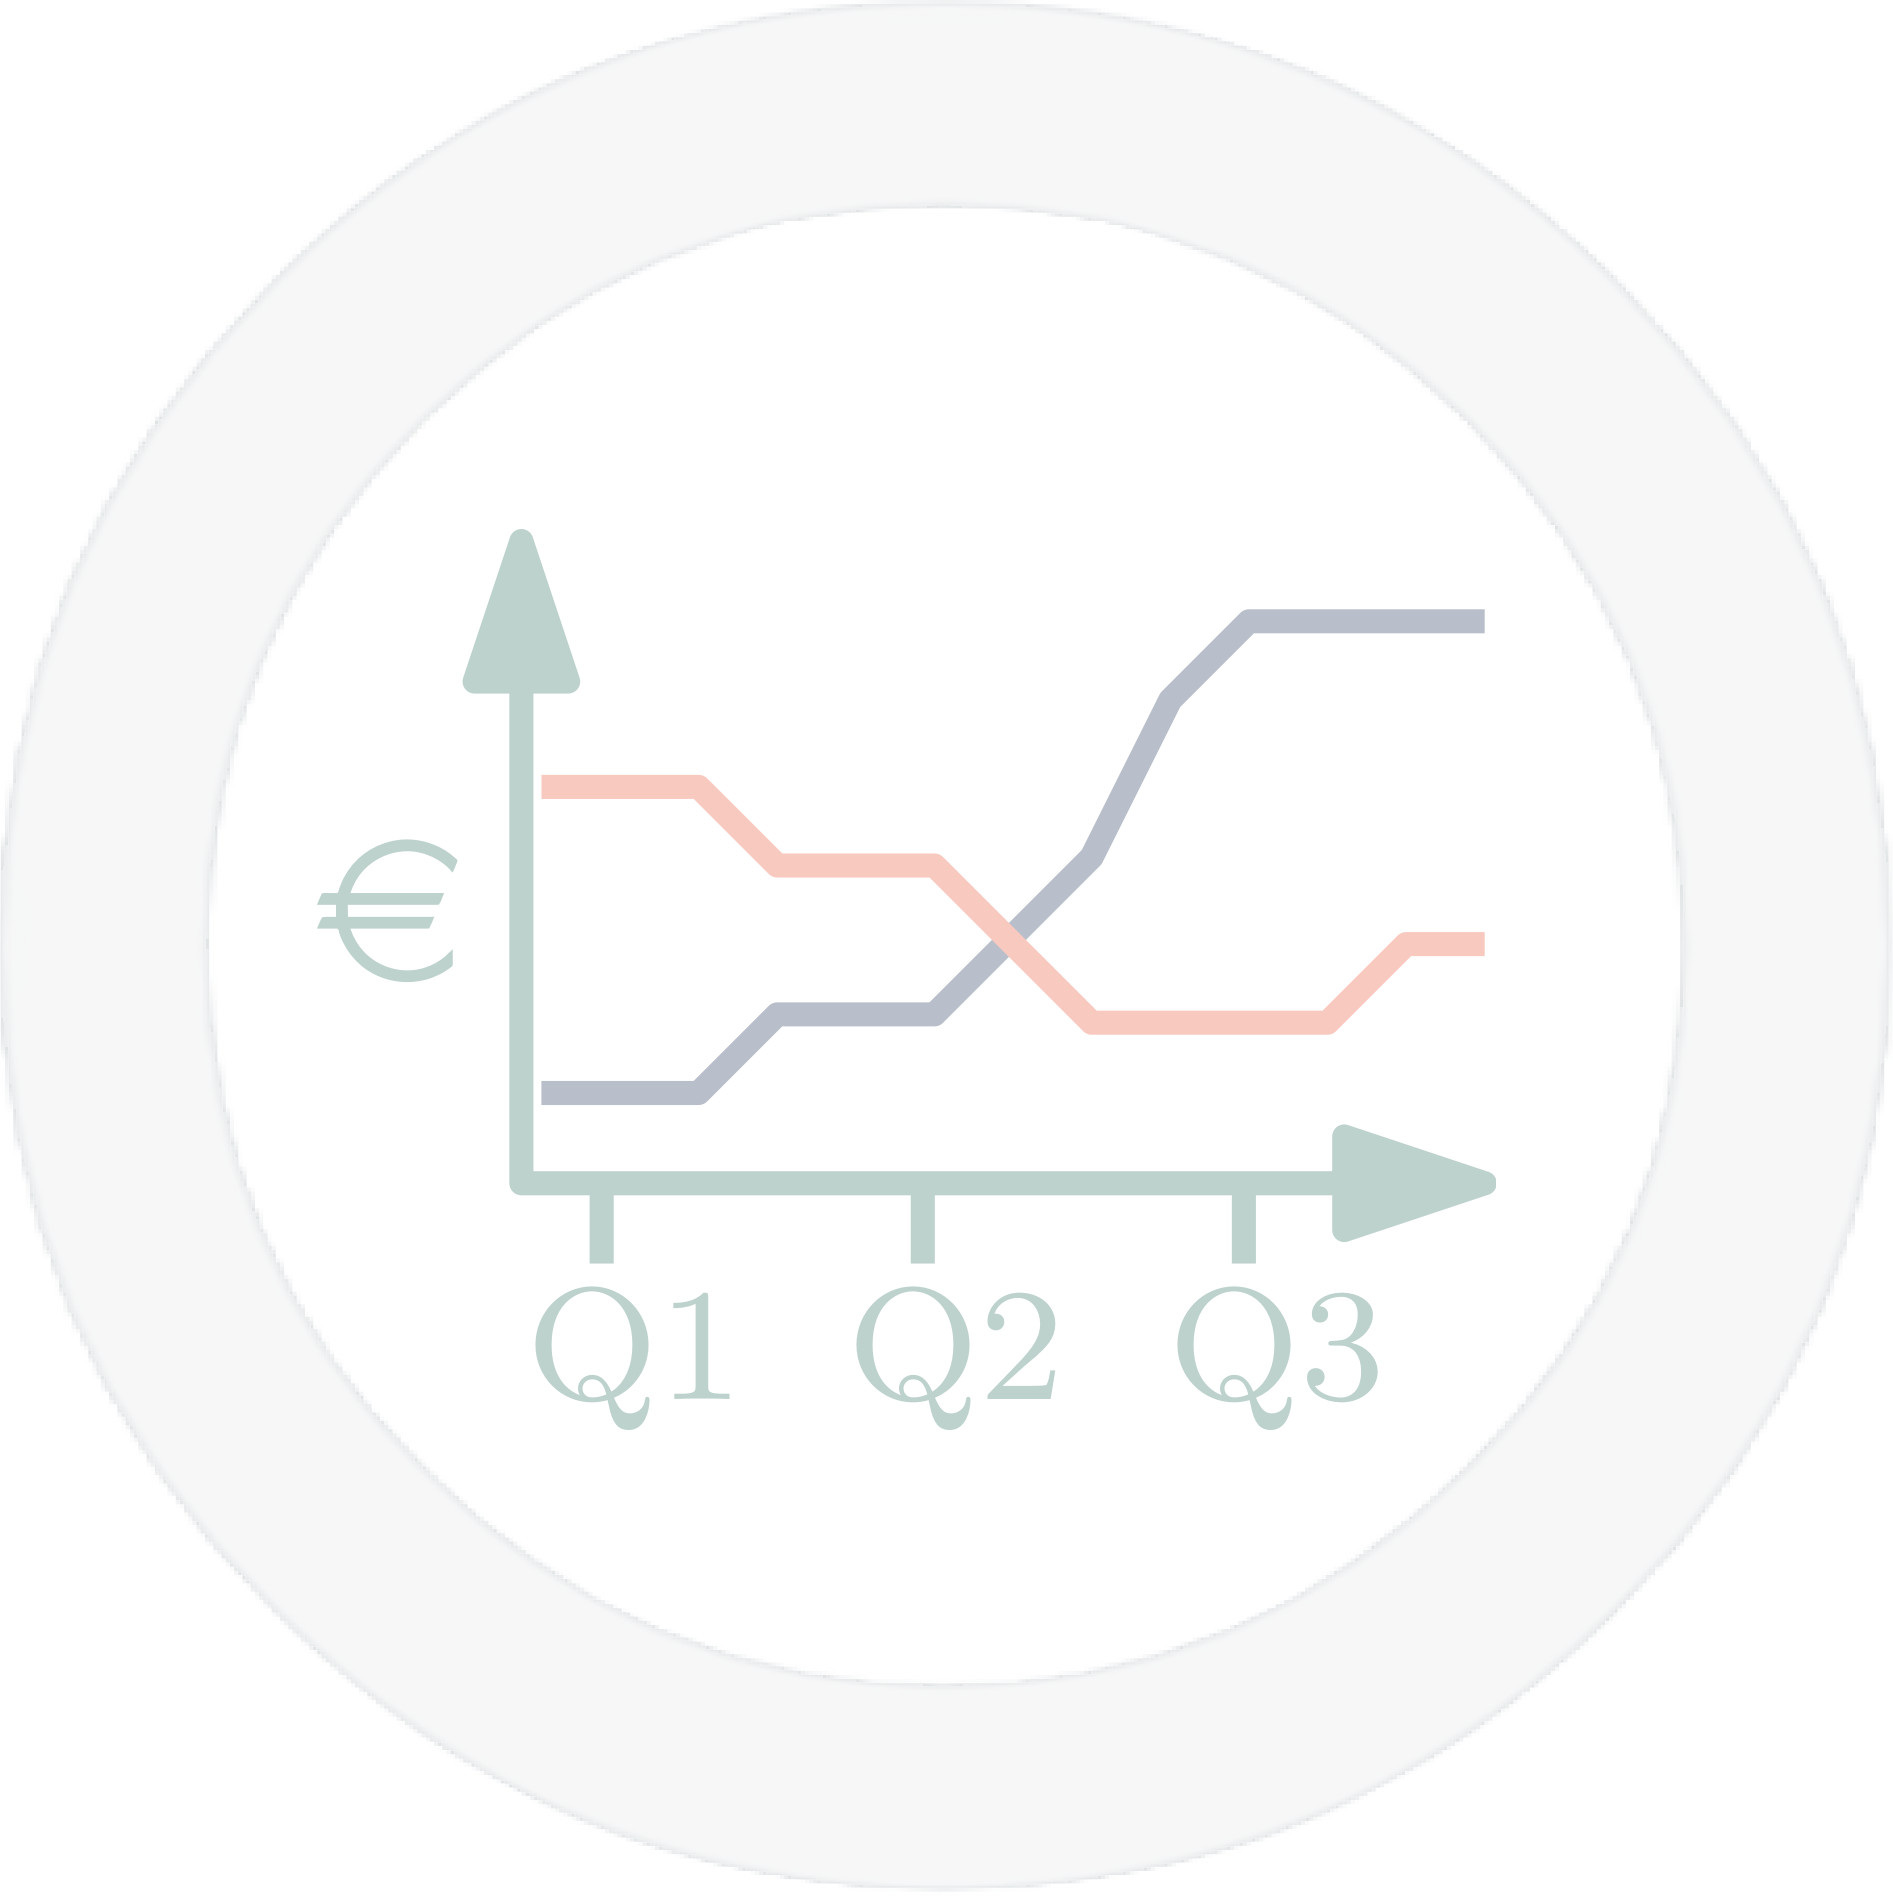
\includegraphics[width=\linewidth]{figures/picture_finance_t.jpg}
			\onslide<3-> 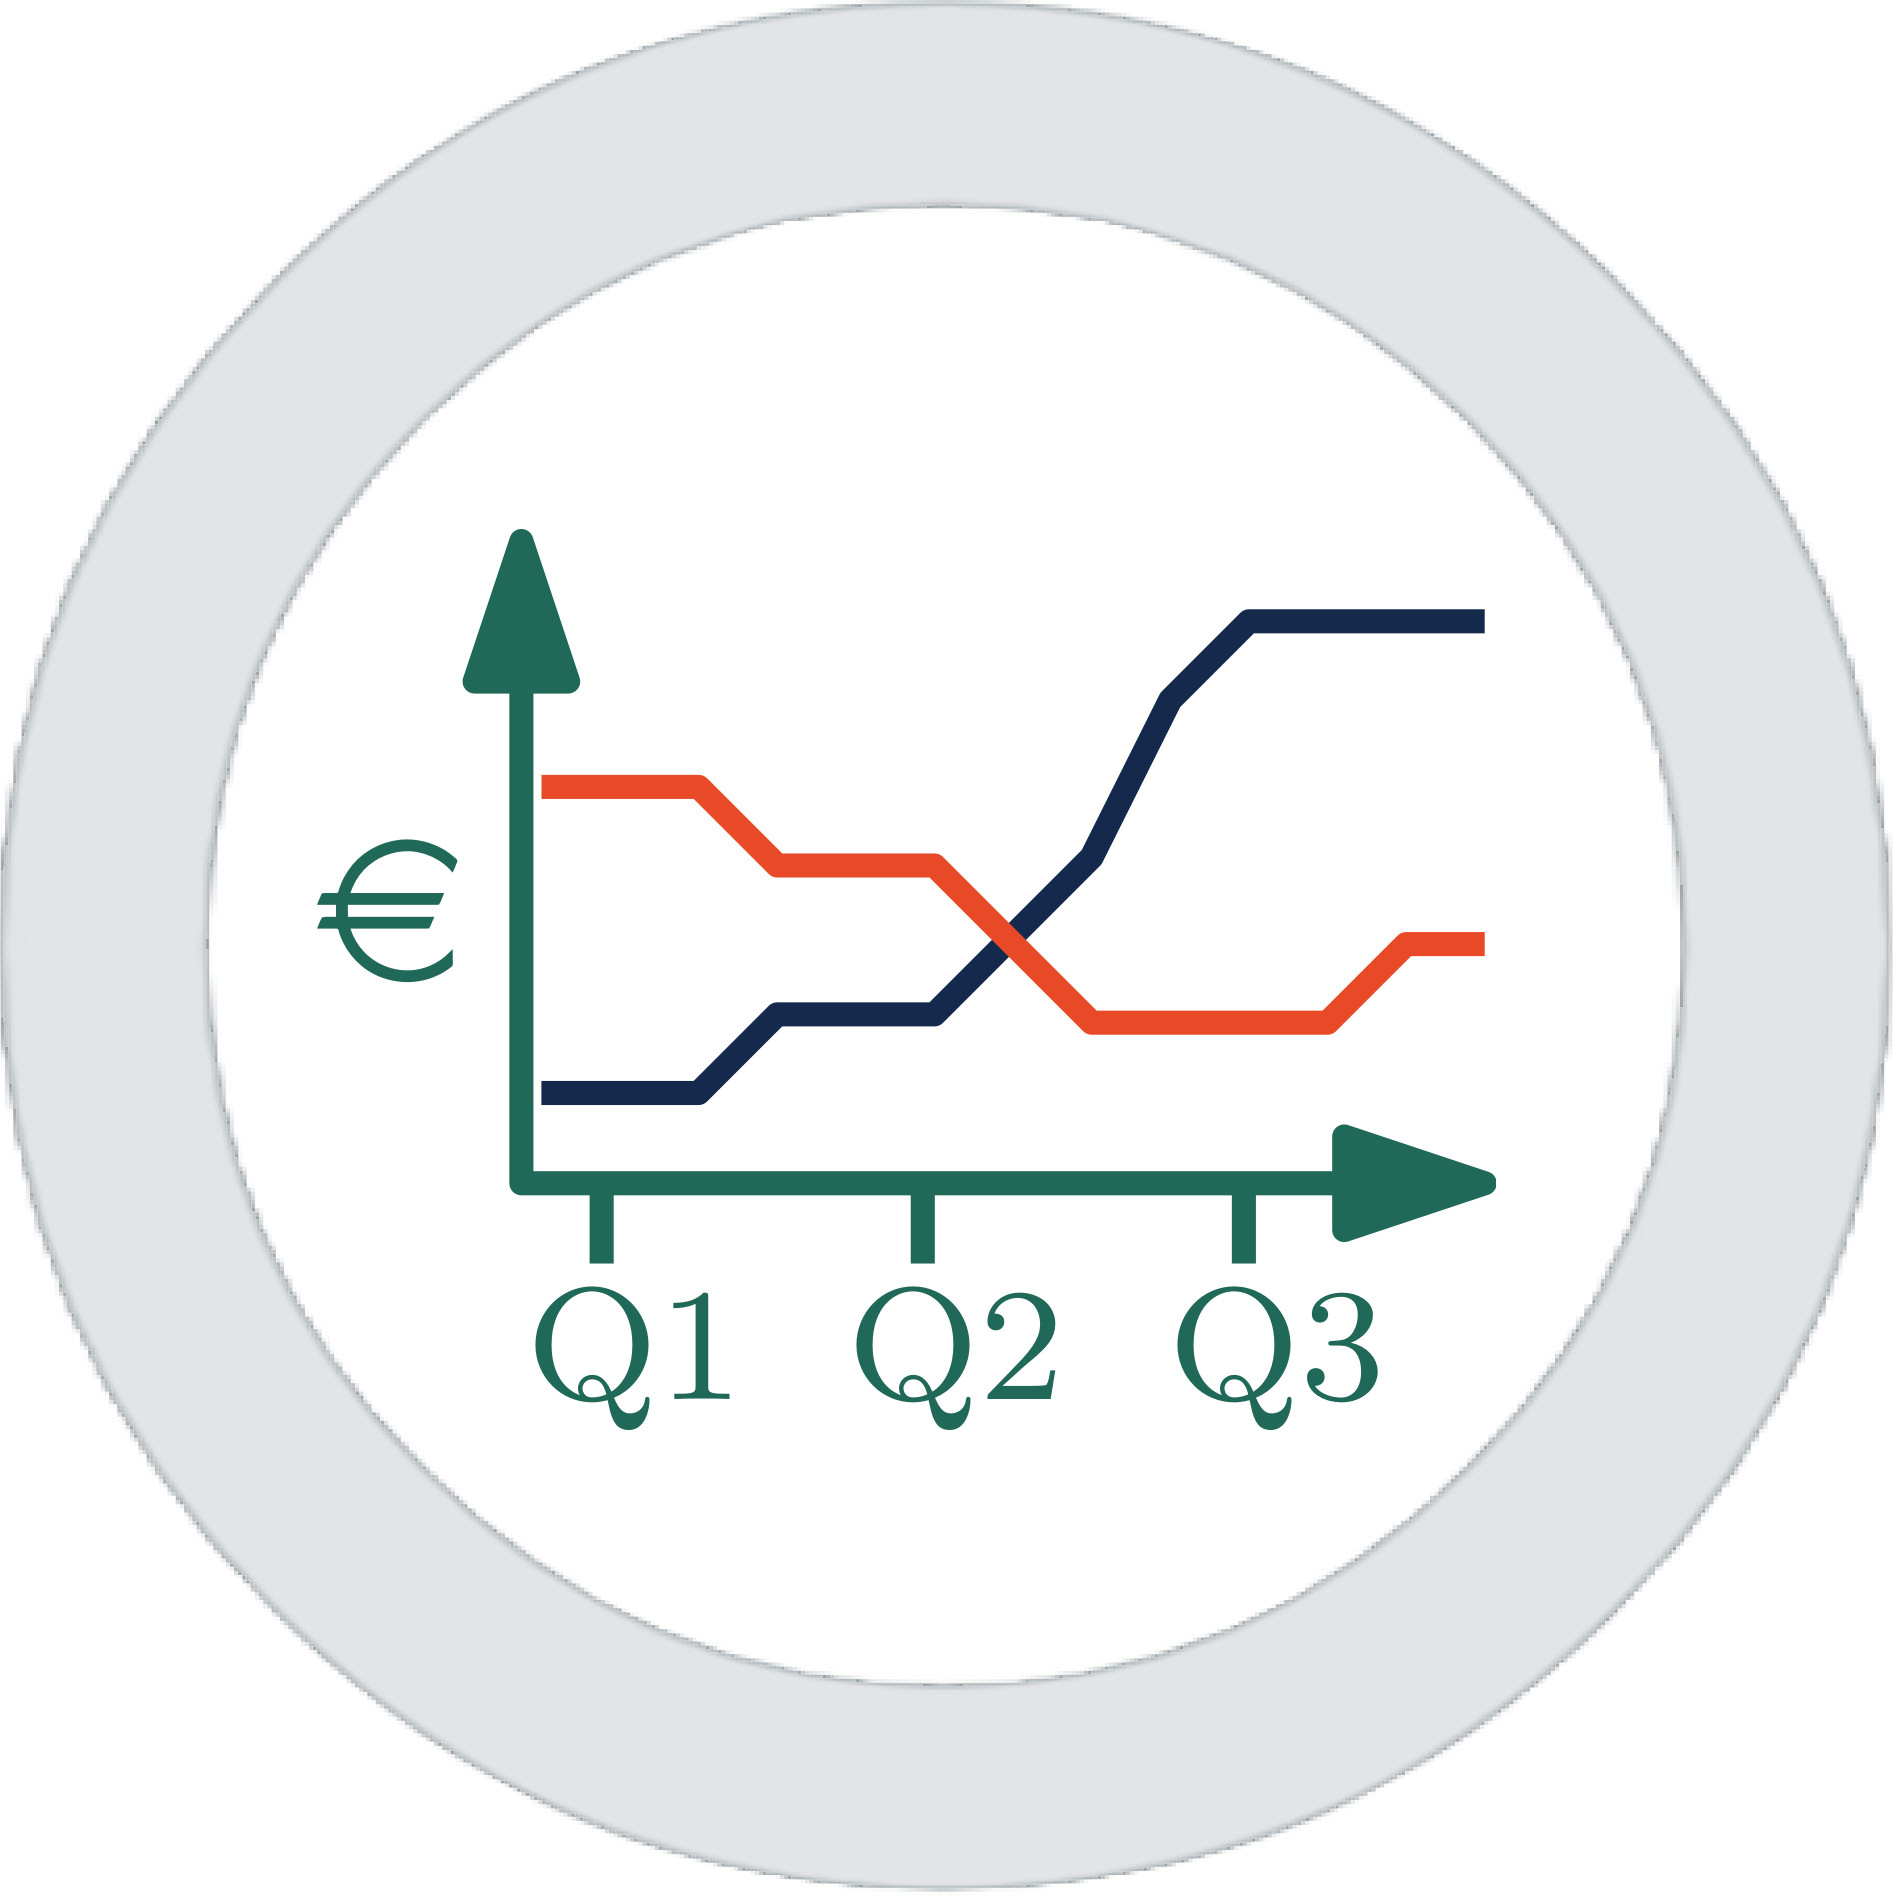
\includegraphics[width=\linewidth]{figures/picture_finance.jpg}
		\end{overprint}
		%\caption*{Finance}
	\end{subfigure}
	\hspace{5mm}
	\begin{subfigure}[c]{0.25\linewidth}
		\centering
		\begin{overprint}
			\onslide<1-3> 
\includegraphics[width=\linewidth]{figures/picture_manufactoring_t.jpg}
			\onslide<4-> 
\includegraphics[width=\linewidth]{figures/picture_manufactoring.jpg}
		\end{overprint}
		%\caption*{Manufacturing}
	\end{subfigure}
\end{figure}
\end{frame}

% Data Mining, also known as Knowledge Discovery, is the process of extracting knowledge from massive data sets. Advances in Data Mining impact our lives in countless ways: 
% For example, it helps to find a cure for human diseases 
% It optimises the advertisement and content we are exposed to, for instance, in social media 
% And it helps to improve the efficiency of industrial production processes, in particular, with the earlier detection of maintenance needs. 

% For example, in Biology,trhe analysis of gene expression from DNA microarray issually involve hundreds to thousands of dimensions
% In finance, understanding the behavior of the market involves deadling with stocks exchange data that is being continuously collected, as a stream. 
% Sometimes, it's even both. For example, in "smart" manufacturing, plants are often equipped with thousands of sensors, delivering new measurements at a possible high sampling rate. 

%\subsection{Challenges}
\begin{frame}{Challenges}

We must deal with \textit{High-Dimensional Data Streams (HD-DS)}. 

$\rightarrow$ They come with two sets of challenges: 
\pause

\begin{columns}
	\begin{column}{0.5\textwidth}
		\begin{center}
			\textbf{High-Dimensionality}
			
			``\textit{curse of dimensionality}'' \cite{bellman1957}
		\end{center}
	\vspace{-0.5cm}
		\begin{itemize}
				\item The space becomes sparse
				\item Number of subspaces $\nearrow$  
				\item \textit{Robust}/\textit{efficient} algorithms
		\end{itemize}
	\end{column}
	\pause
	\begin{column}{0.5\textwidth}  %%<--- here
		\vspace{-0.70cm}
		\begin{center}
			 \textbf{Data Streams}
			
			``\textit{concept drift}'' \cite{DBLP:conf/ictai/BarddalGE15}
		\end{center}
	\vspace{-0.5cm}
		\begin{itemize}
			\item Data may change over time 
			\item \textit{Adaptive} techniques
		\end{itemize}
	\end{column}
\end{columns}

~\\
~\\
~\\
~\\
~\\

\begin{overprint}
	\onslide<1> \begin{tikzpicture}[remember picture,overlay, opacity=0.3]
	\node[anchor=south east,inner sep=0pt] at ($(current page.south east)+(-7.2cm,0.8cm)$) {
		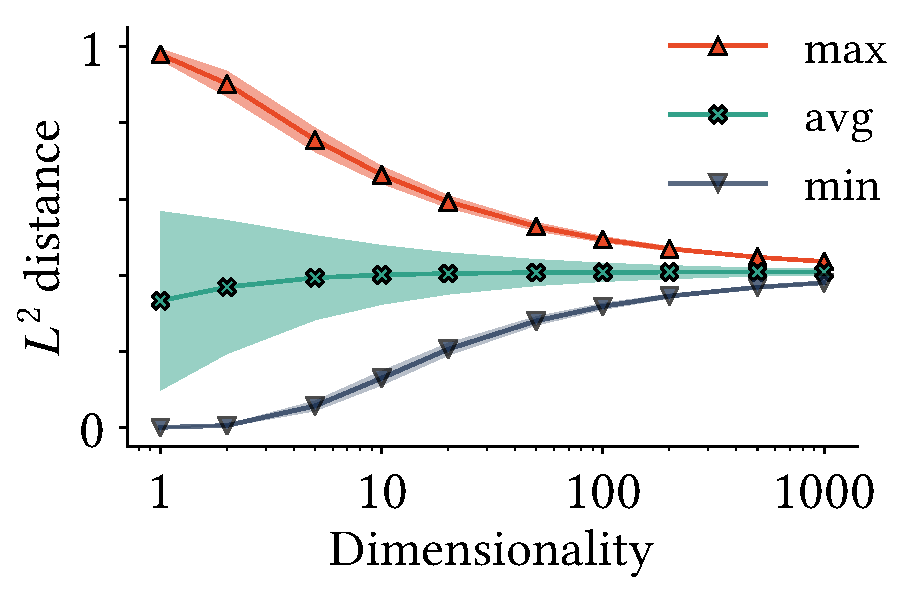
\includegraphics[width=0.42\linewidth]{figures/cod_illustration_2-compressed.pdf}
		
	};
	\end{tikzpicture}
	\onslide<2-> \begin{tikzpicture}[remember picture,overlay]
\node[anchor=south east,inner sep=0pt] at ($(current page.south east)+(-7.2cm,0.8cm)$) {
	 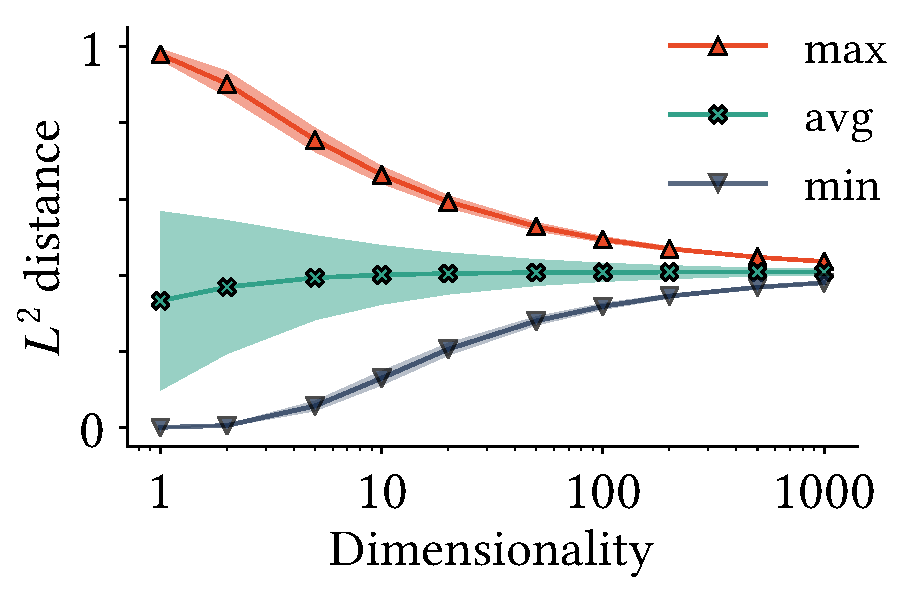
\includegraphics[width=0.42\linewidth]{figures/cod_illustration_2-compressed.pdf}
	
};
\end{tikzpicture}
\end{overprint}

\begin{overprint}
	\onslide<1-2> \begin{tikzpicture}[remember picture,overlay, opacity=0.3]
	\node[anchor=south east,inner sep=0pt] at ($(current page.south east)+(0cm,1.2cm)$) {
		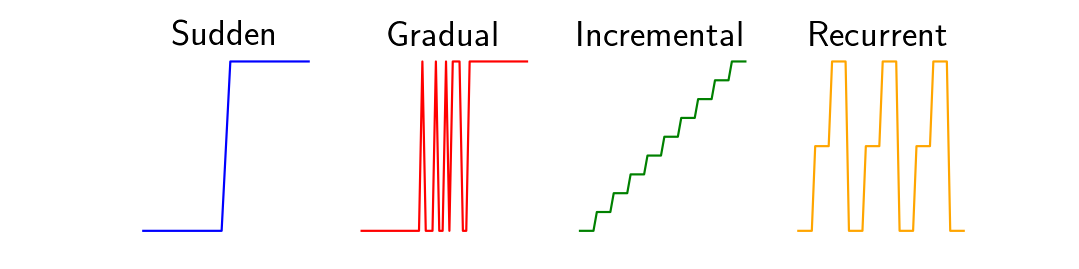
\includegraphics[angle=0, width=7cm]{figures/conceptdrift_row.png}
	};
	\end{tikzpicture}
	\onslide<3-> \begin{tikzpicture}[remember picture,overlay]
\node[anchor=south east,inner sep=0pt] at ($(current page.south east)+(0cm,1.2cm)$) {
	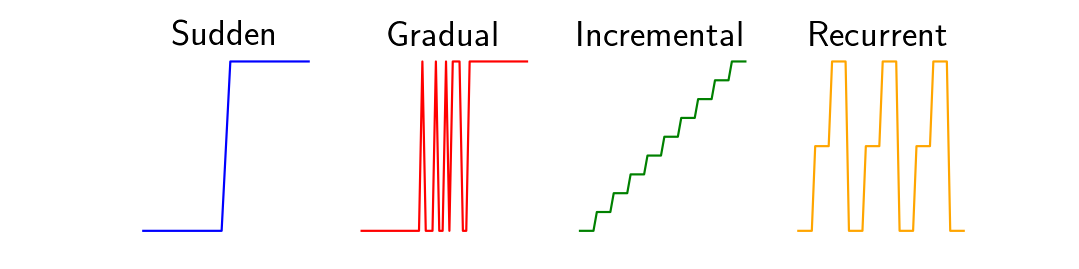
\includegraphics[angle=0, width=7cm]{figures/conceptdrift_row.png}
};
\end{tikzpicture}
\end{overprint}

\begin{overprint}
	\onslide<1-2> \begin{tikzpicture}[remember picture,overlay, opacity=0.3]
	\node[anchor=south east,inner sep=0pt] at ($(current page.south east)+(-1.0cm,3.1cm)$) {
		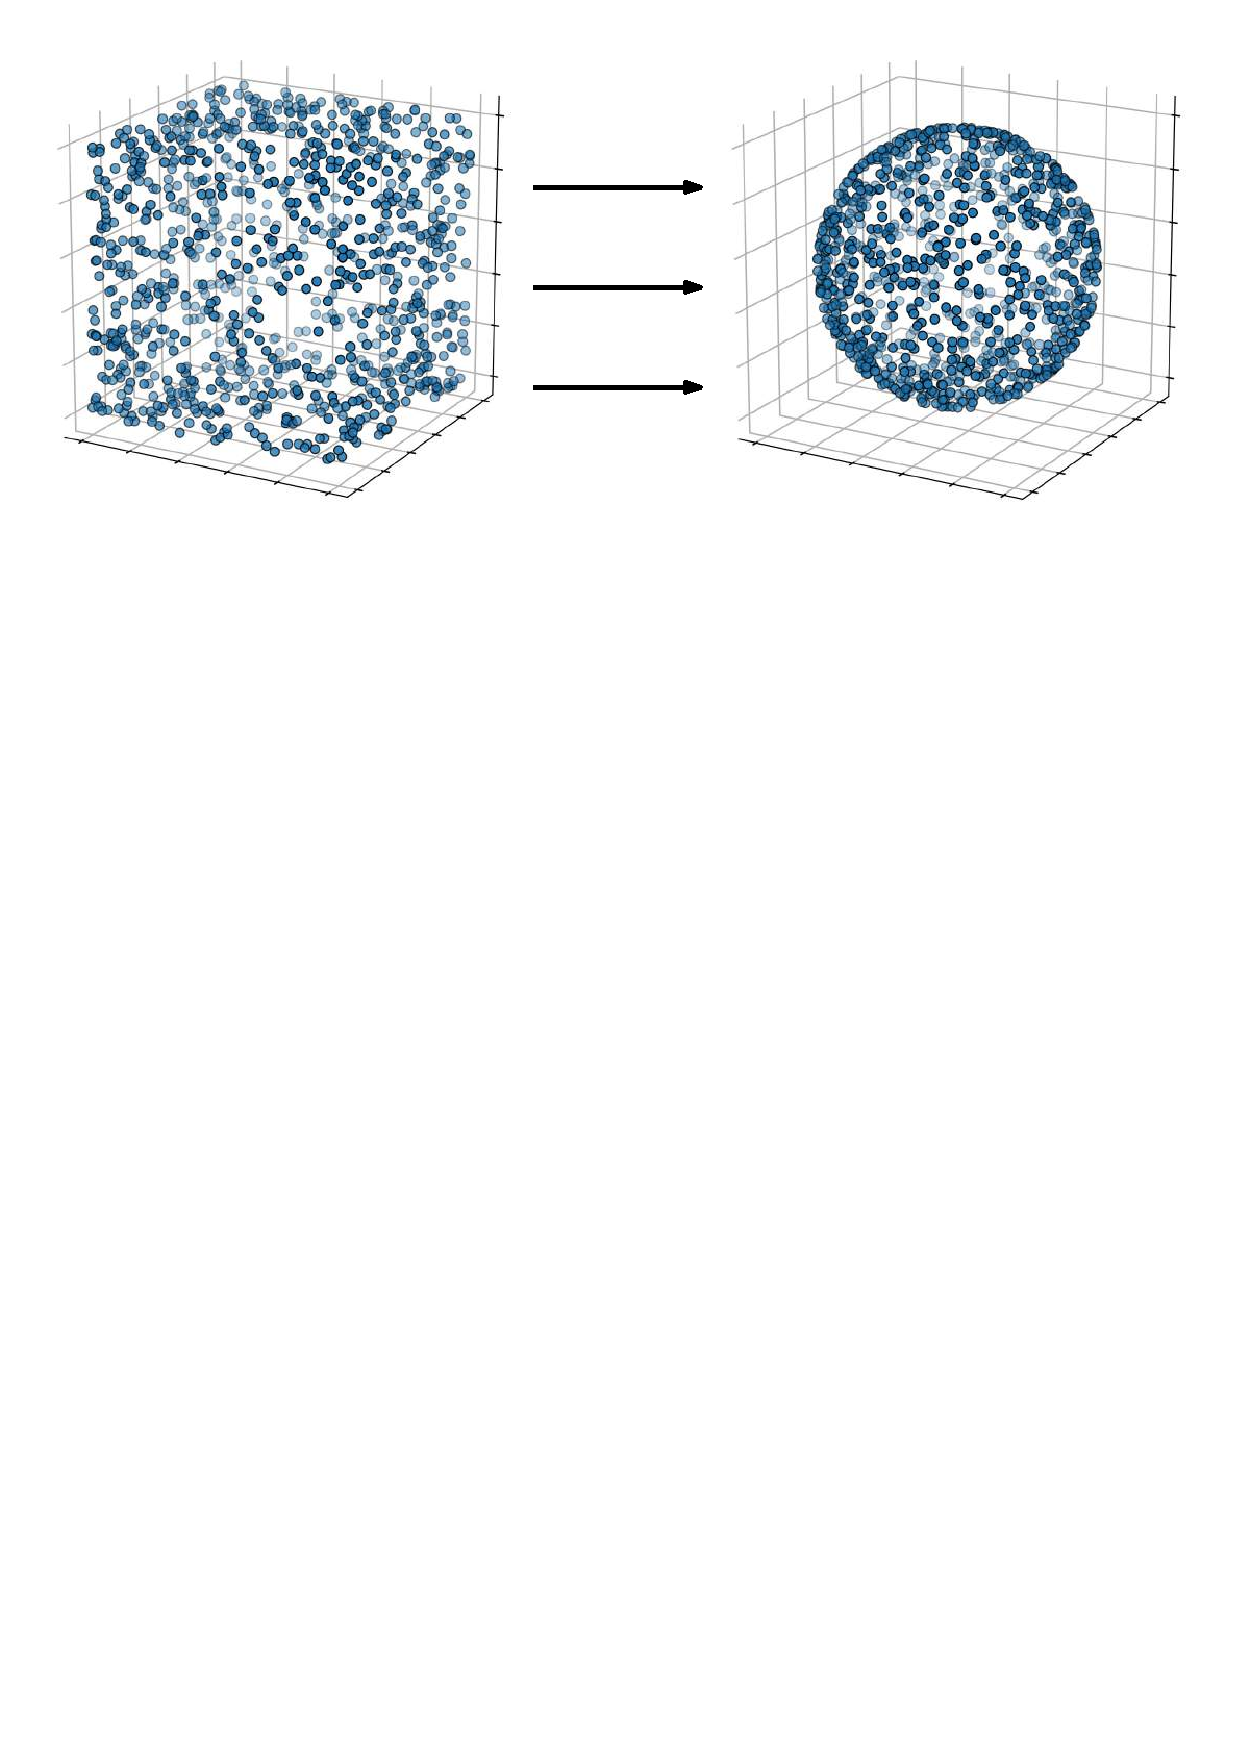
\includegraphics[angle=0, width=4.5cm]{figures/conceptdrift_example-compressed.pdf}
	};
	\end{tikzpicture}
	\onslide<3-> \begin{tikzpicture}[remember picture,overlay]
	\node[anchor=south east,inner sep=0pt] at ($(current page.south east)+(-1.0cm,3.1cm)$) {
		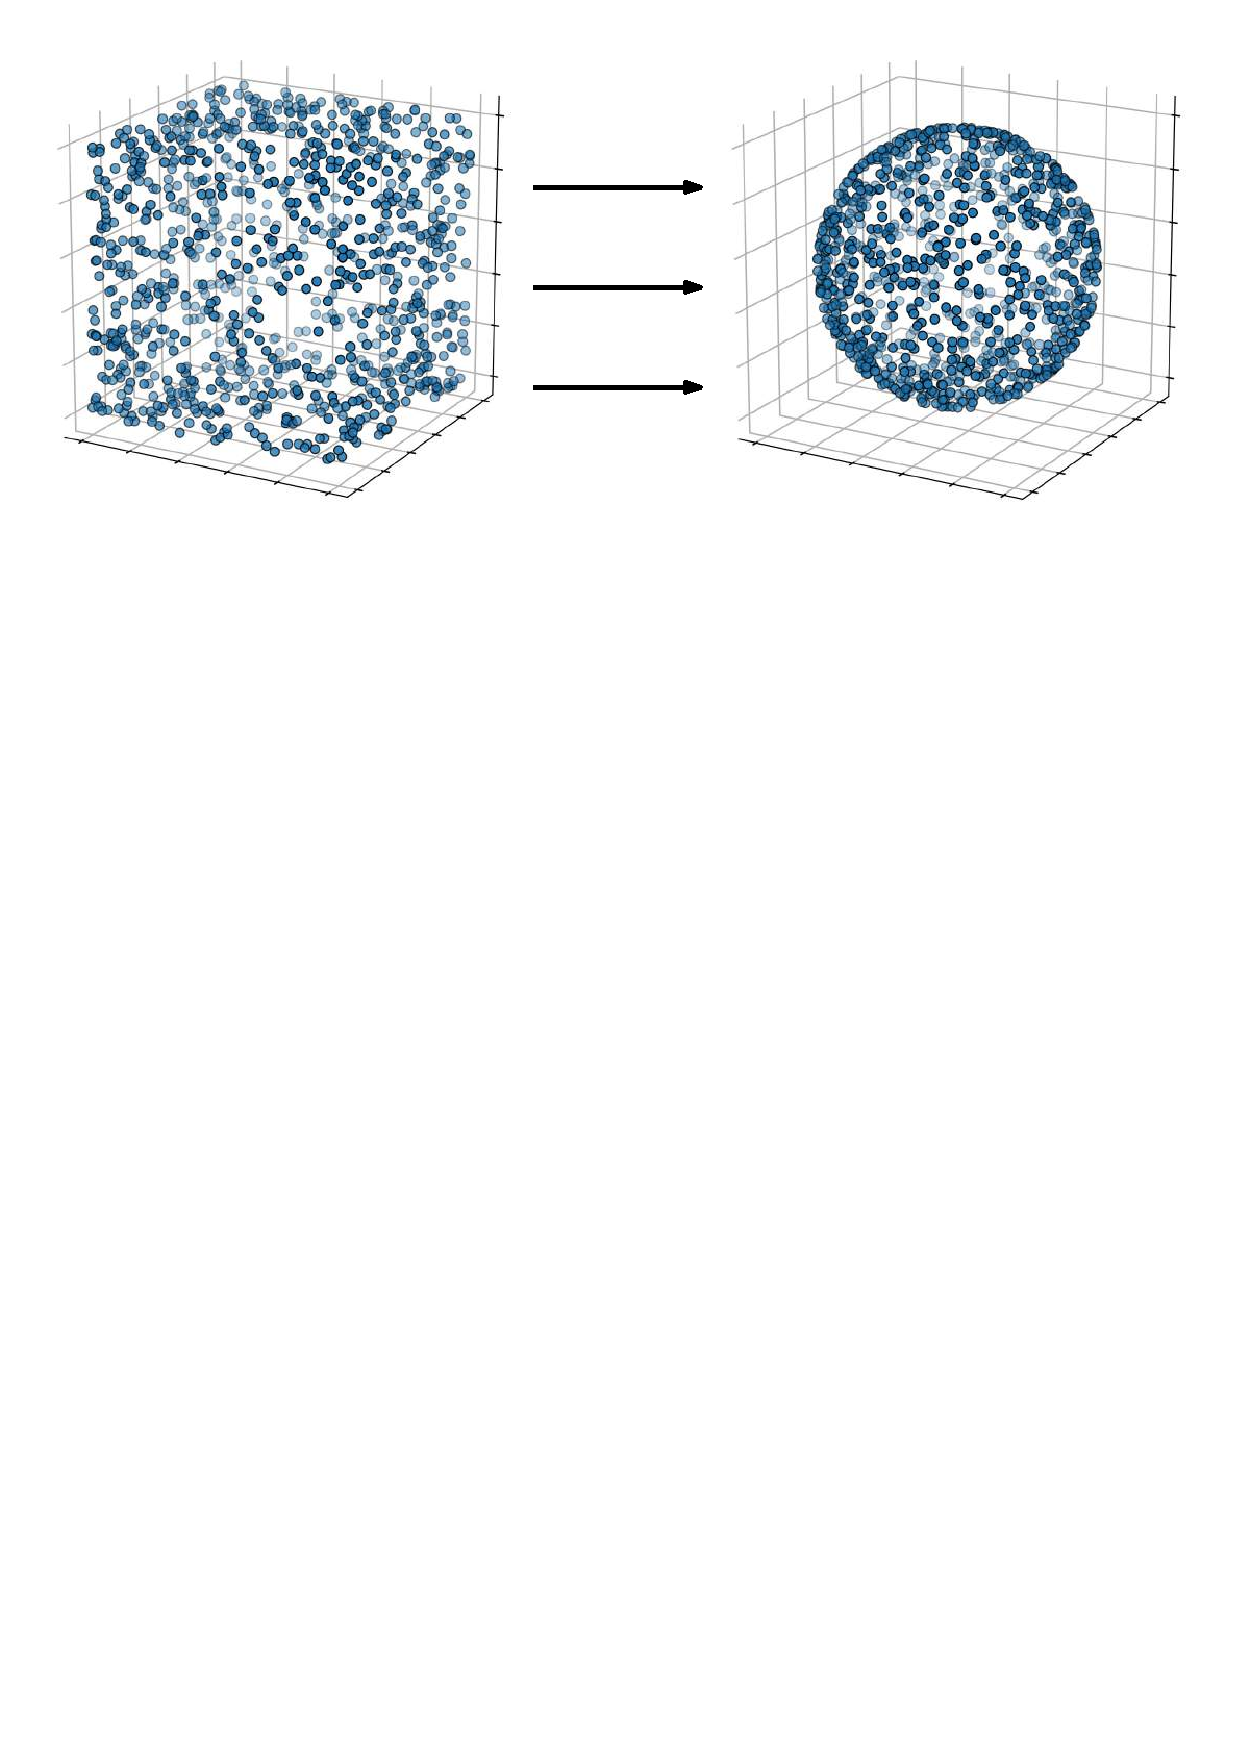
\includegraphics[angle=0, width=4.5cm]{figures/conceptdrift_example-compressed.pdf}
	};
	\end{tikzpicture}
\end{overprint}

~\\

\end{frame}
% However, modern tasks often involve High-Dimensional Data Streams, which comes with two sets of specifics and distinct challenges: 
% On the one hand, with high-dimensional data, several effects, commonly known as the ``curse of dimensionality'', challenge Knowledge Discovery. The space becomes extremely sparse, objects tend to be all similarly close to each other, and the number of attribute pairs or subspaces increases dramatically. Here, on the right, we show an example of the so-called distance concentration effects: As dimensionality increases, we can see that the distances between uniformly distributed points in a high-dimensional data space all converge to the same value. The bottom line is that we need algorithms which are robust to such effects and efficient at the same time. 
% On the other hand, in the Data Streams, the characteristics of data changes in unexpected ways, a phenomenon known as concept drift. This phenomenon may occur in many different ways, so we need adaptive techniques. 

\begin{frame}{Focus of other works}

\begin{figure}
	\centering
	\begin{overprint}
		\onslide<1> 
		\centering
		\begin{tikzpicture}[thick]
		\draw (2.5,2.25) node { High};
		\draw (2.5,1.75) node { Dimensionality};
		\draw (2.5,2) circle (2.5cm);
		
		\draw (6.5,2) circle (2.5cm);
		\draw (6.5,2.25) node { Data};
		\draw (6.5,1.75) node { Streams};
		\end{tikzpicture}
		\onslide<2->
		\centering
		\begin{tikzpicture}[thick]
		\begin{scope}
		\clip (2.5,2) circle (2.5cm);
		\fill[pattern=crosshatch, pattern color=uiucred] (6.5,2) circle (2.5cm);
		\end{scope}
		\draw (2.5,2.25) node { High};
		\draw (2.5,1.75) node { Dimensionality};
		\draw (2.5,2) circle (2.5cm);
		
		\draw (6.5,2) circle (2.5cm);
		\draw (6.5,2.25) node { Data};
		\draw (6.5,1.75) node { Streams};
		\draw[thick,->] (4.5,0.0) -- (4.5,1.5);
		\draw (4.5,-0.5)  node {\Huge \textcolor{uiucred}{\textsc{\textbf{?}}}};
		\end{tikzpicture}
	\end{overprint}
	\label{unexplored}
\end{figure}

\pause
\begin{center}
	This is the central interrogation of this dissertation
\end{center}
\end{frame}
% The problem is that, when looking at existing methods, it turns out that their either target at solving the problems linked to high-dimensionality or the streaming setting. And unfortunately, only a few works are dealing with issues at the intersection of both. 
% This observation forms the starting point of my dissertation. I want to bridge this gap by proposing fundamental algorithms addressing both sets of challenges simultaneously. One can then use such algorithms as a basis for solving problems in high-dimensional data streams. 

%\subsection{Examples}
\begin{frame}{The Role of Dependency Estimation}
\begin{itemize}
	\item Dependency/Correlation:
	\begin{itemize}
		\item Describes the strength of relationship between attributes
		\item In practice: Can only be \textcolor{uiucred}{estimated} from empirical observations
		\item Examples: Pearson, Spearman, Mutual Information (MI), \dots
	\end{itemize}
	\pause
	\item Plays a central role in the KDD process
\end{itemize}
\vspace{-1.0cm}
\begin{figure}
	\begin{overprint}
		\onslide<2> 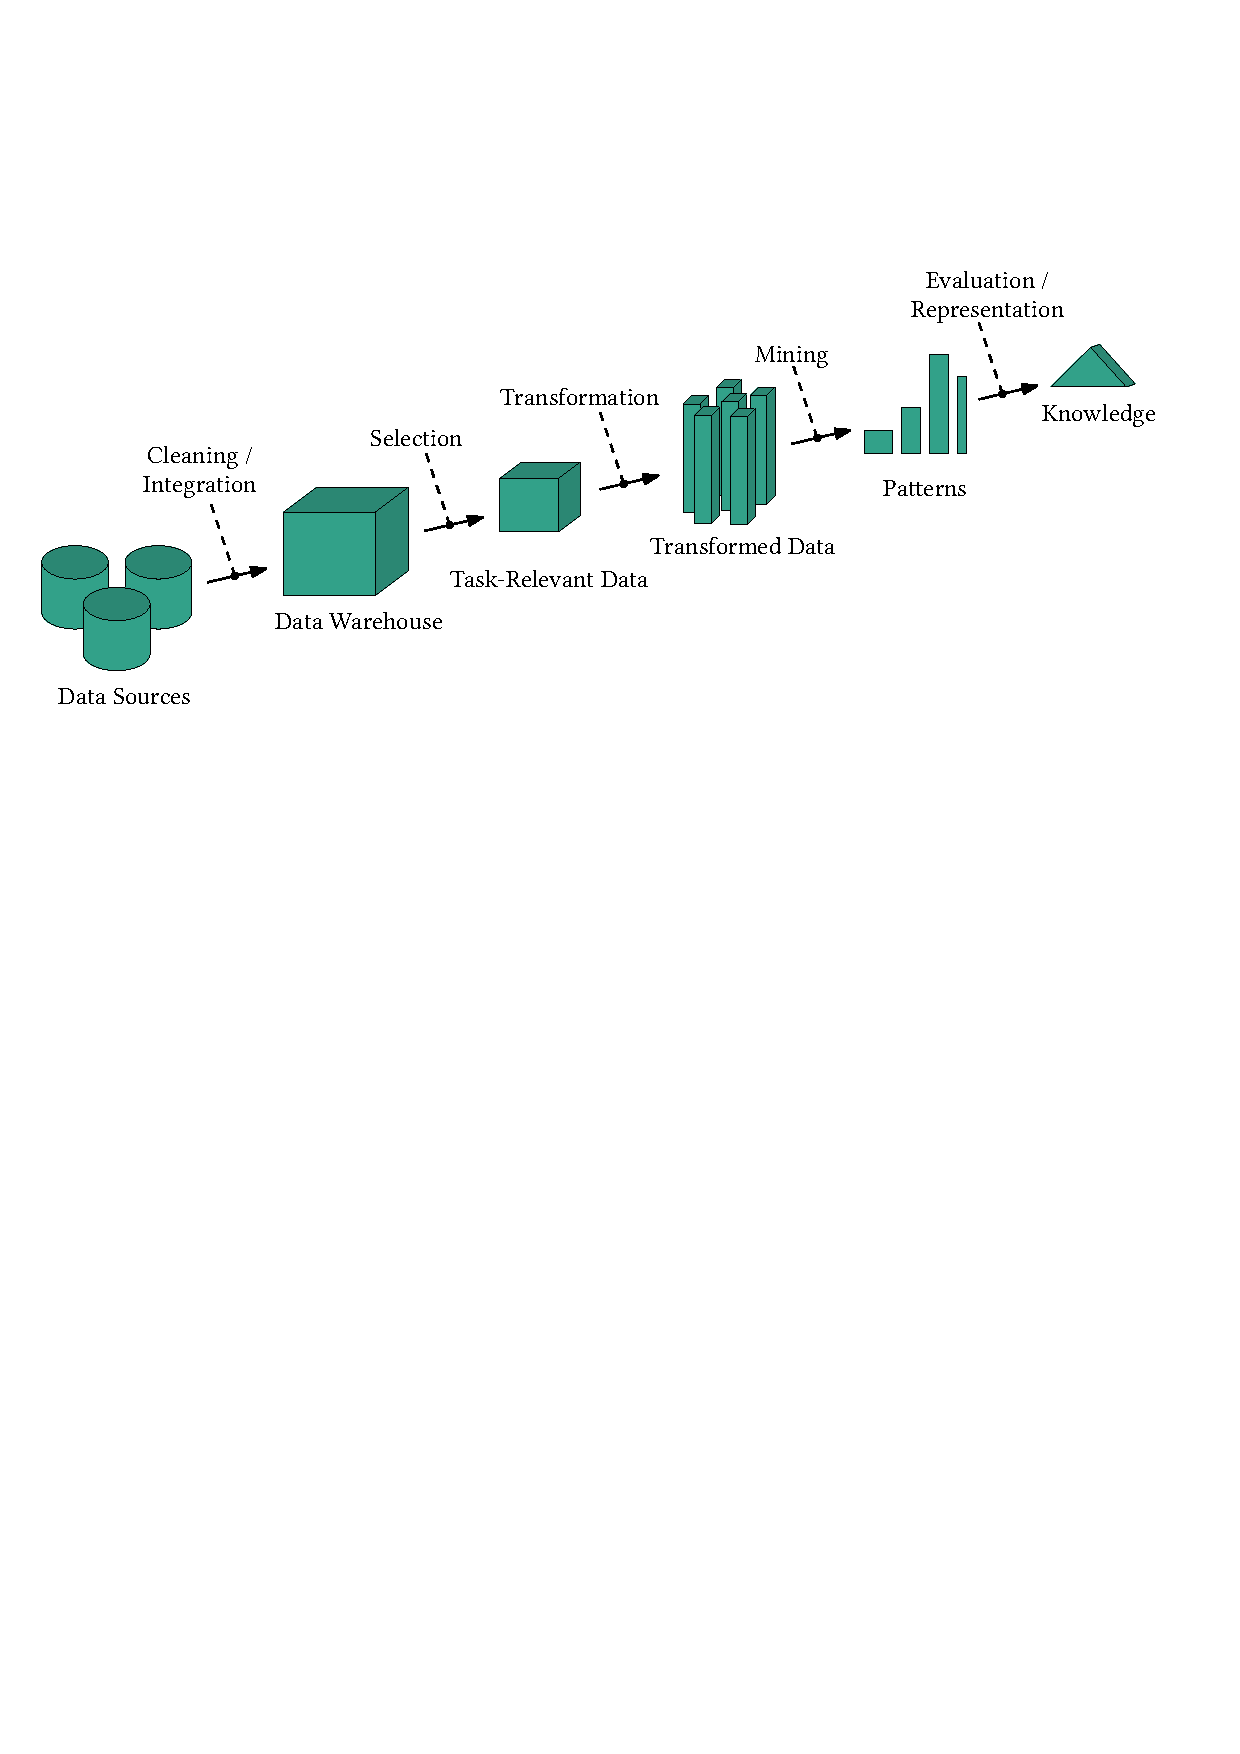
\includegraphics[width=0.98\linewidth]{figures/kdd_5-compressed.pdf}
		\onslide<3> 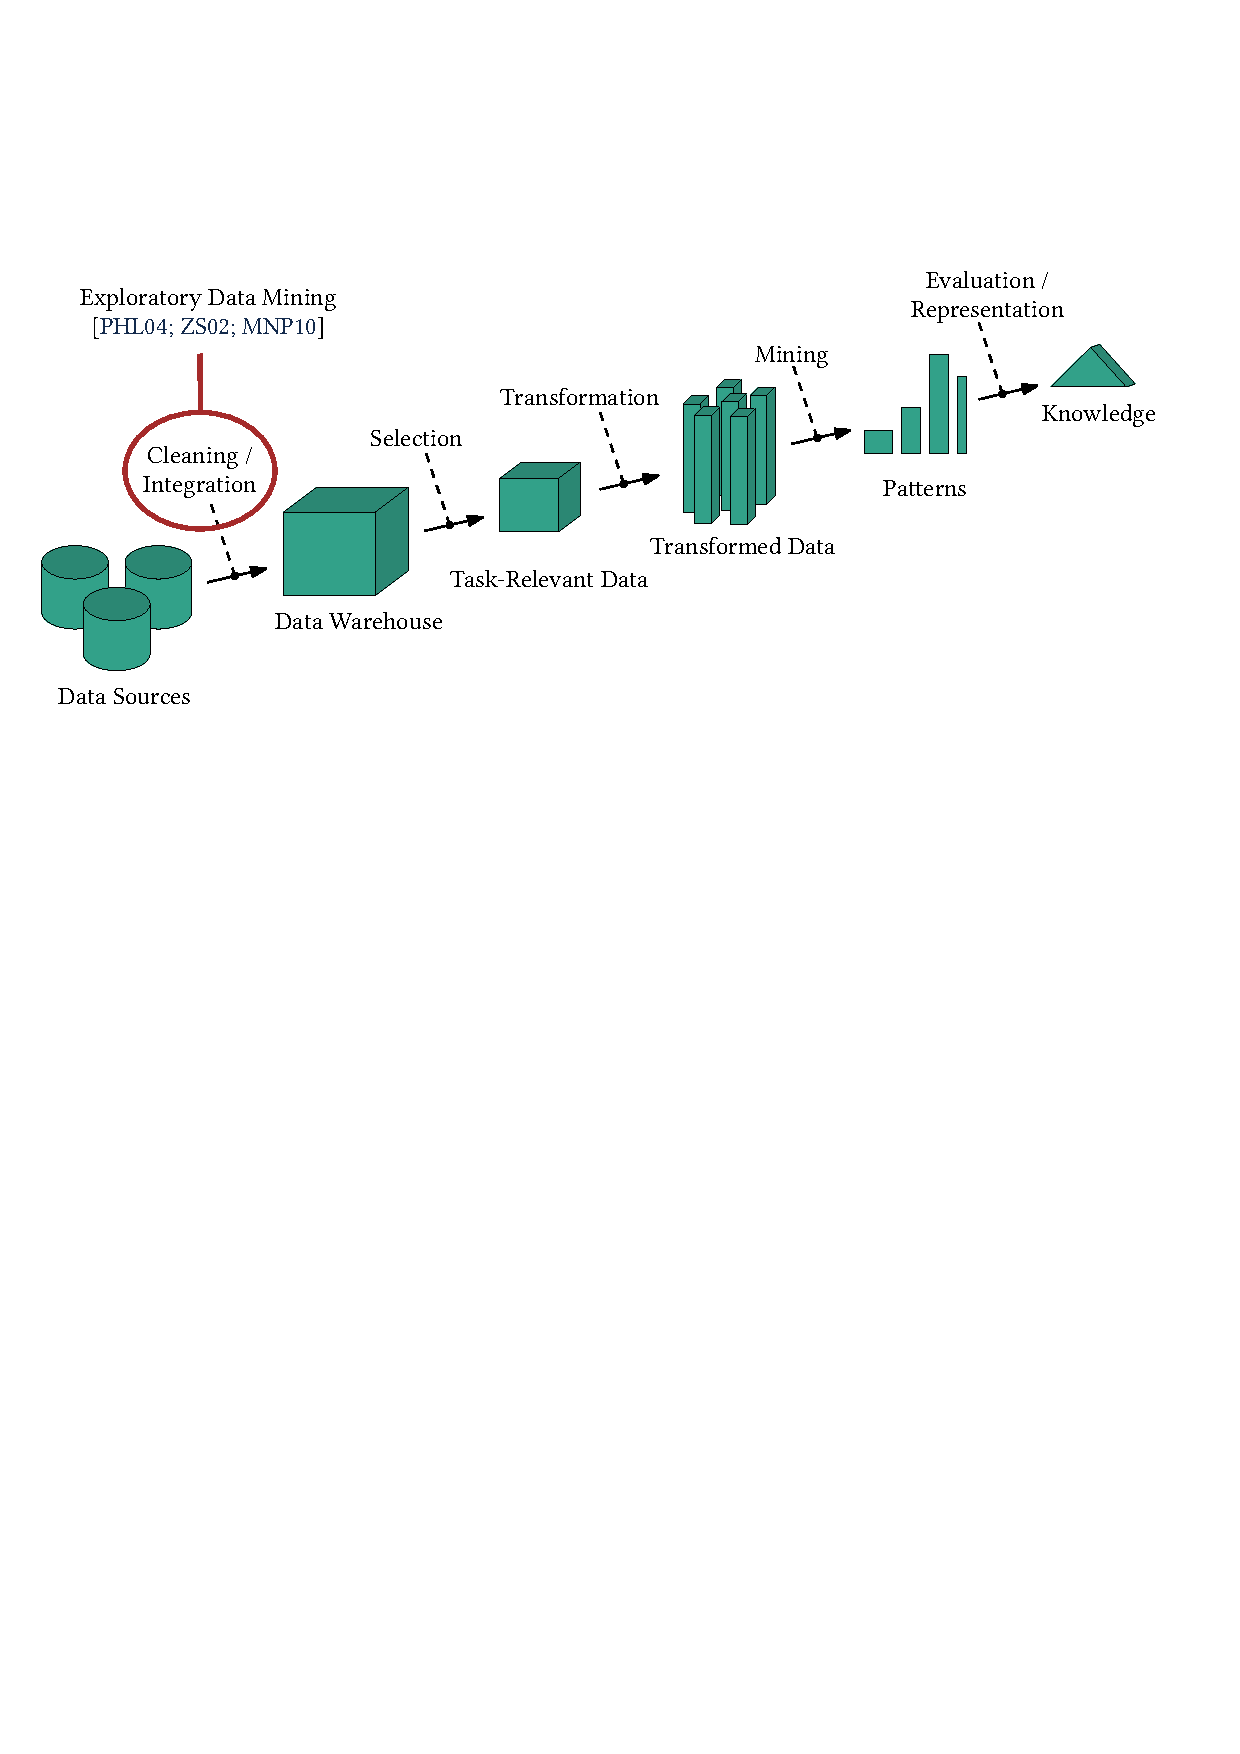
\includegraphics[width=0.98\linewidth]{figures/kdd_r1-compressed.pdf}
		\onslide<4> 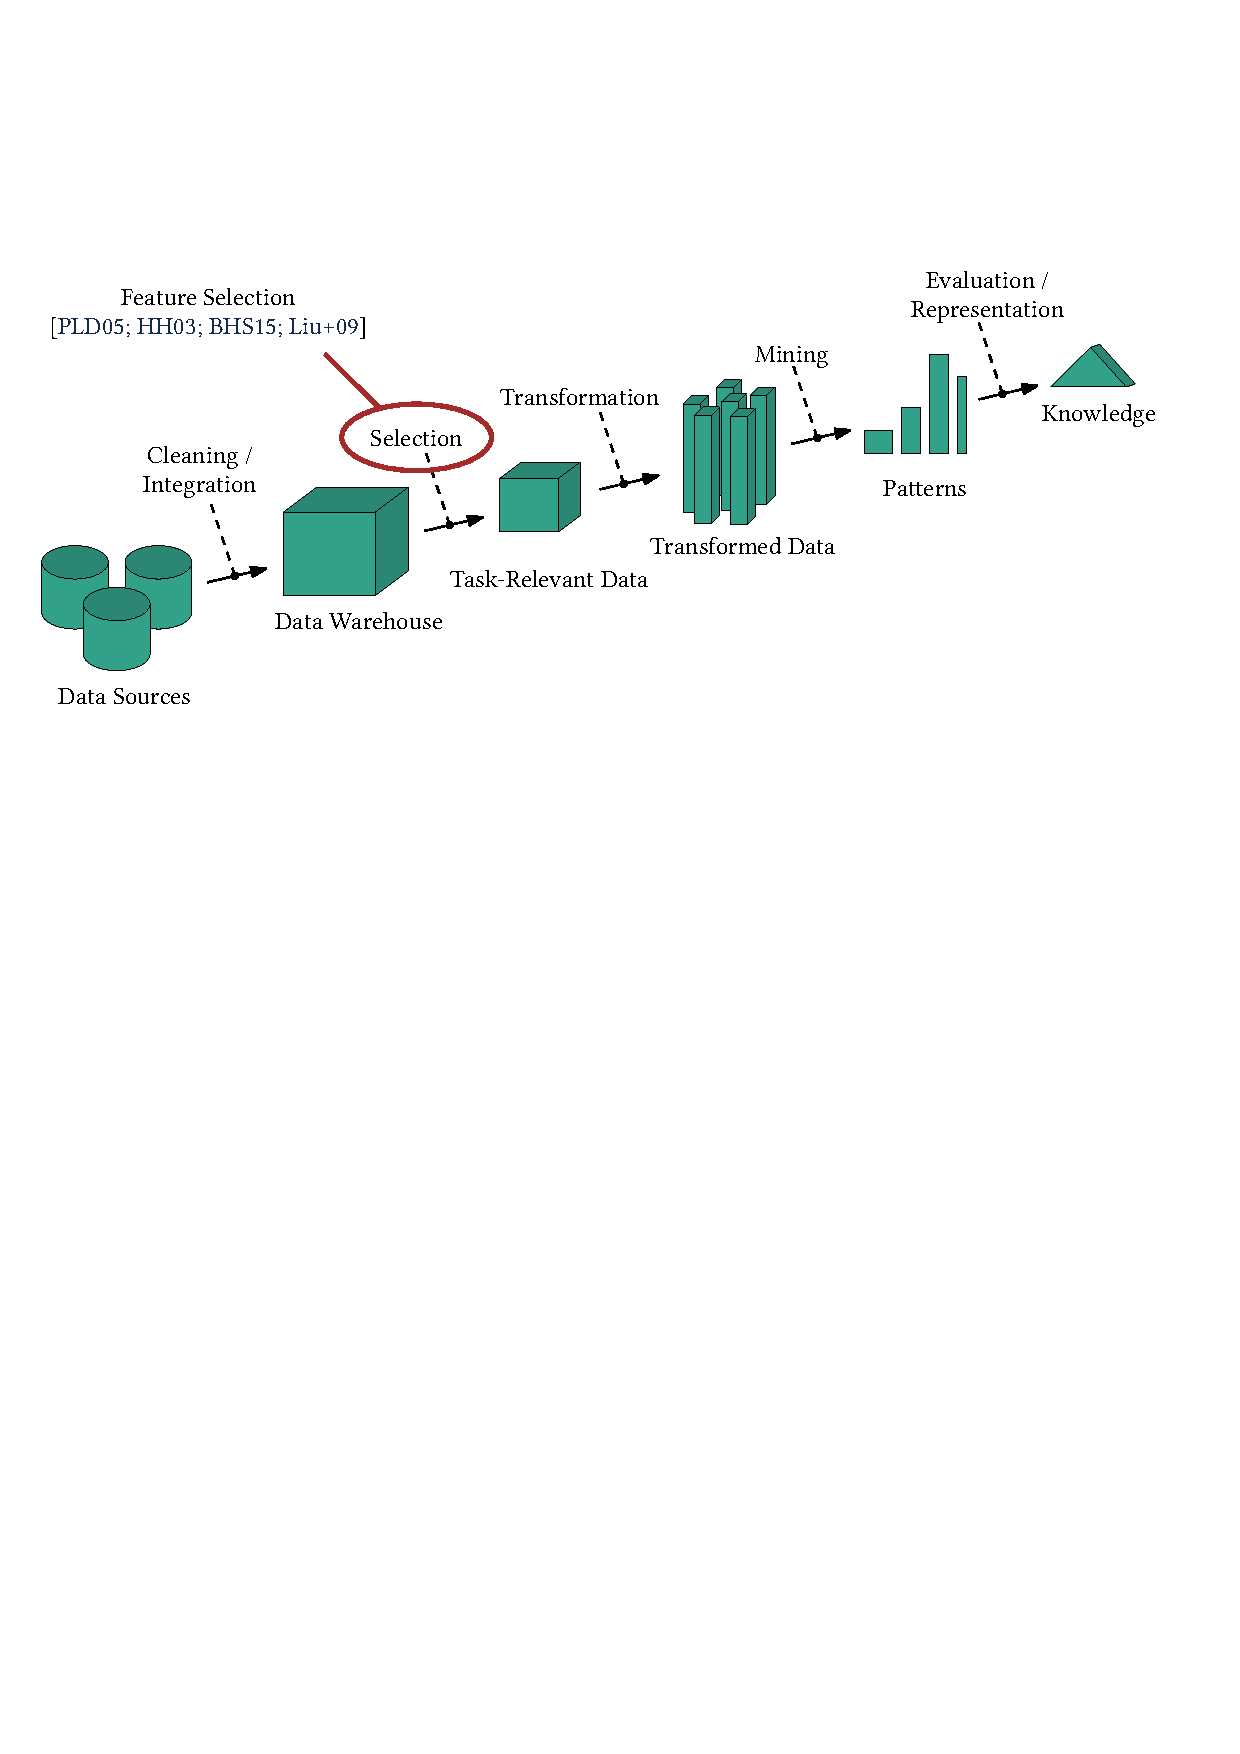
\includegraphics[width=0.98\linewidth]{figures/kdd_r2-compressed.pdf}
		\onslide<5> 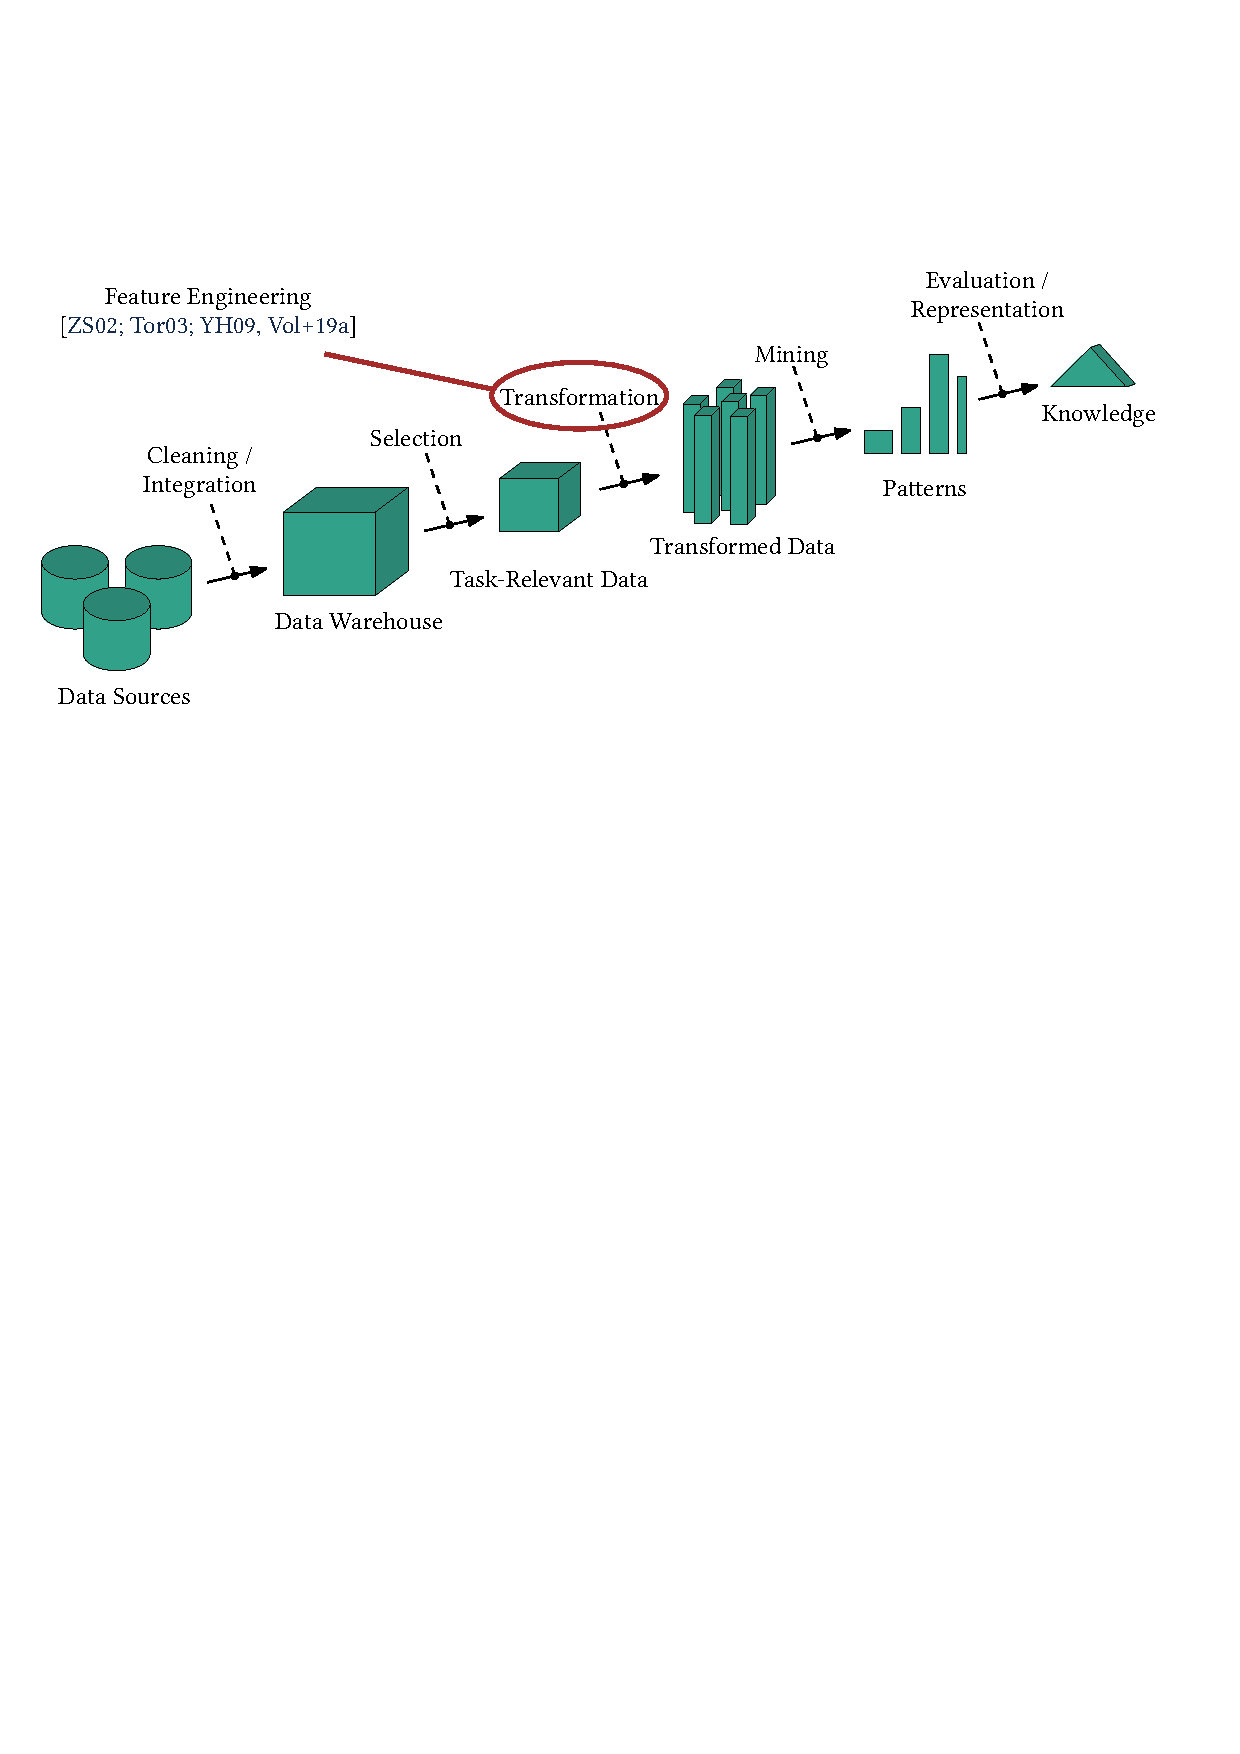
\includegraphics[width=0.98\linewidth]{figures/kdd_r3-compressed.pdf}
		\onslide<6> 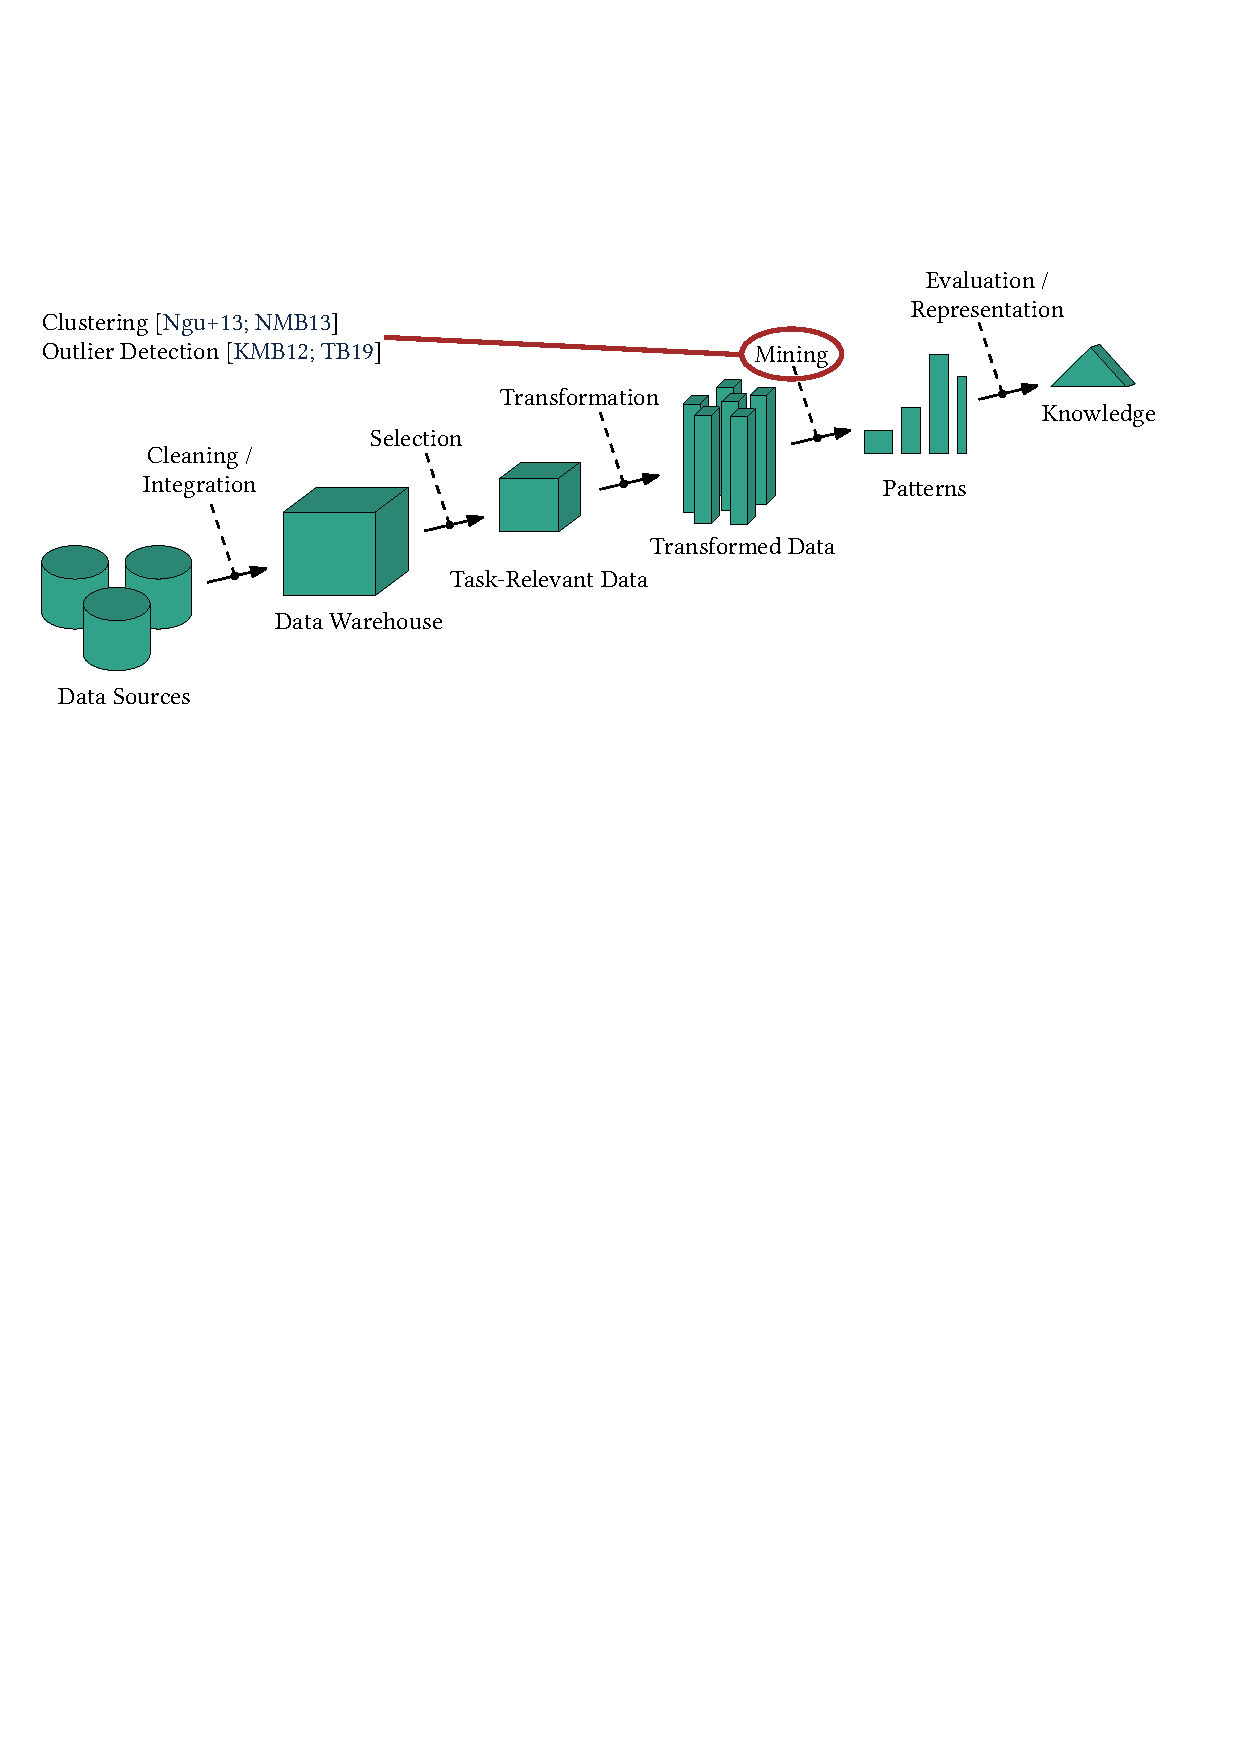
\includegraphics[width=0.98\linewidth]{figures/kdd_r4-compressed.pdf}
		\onslide<7> 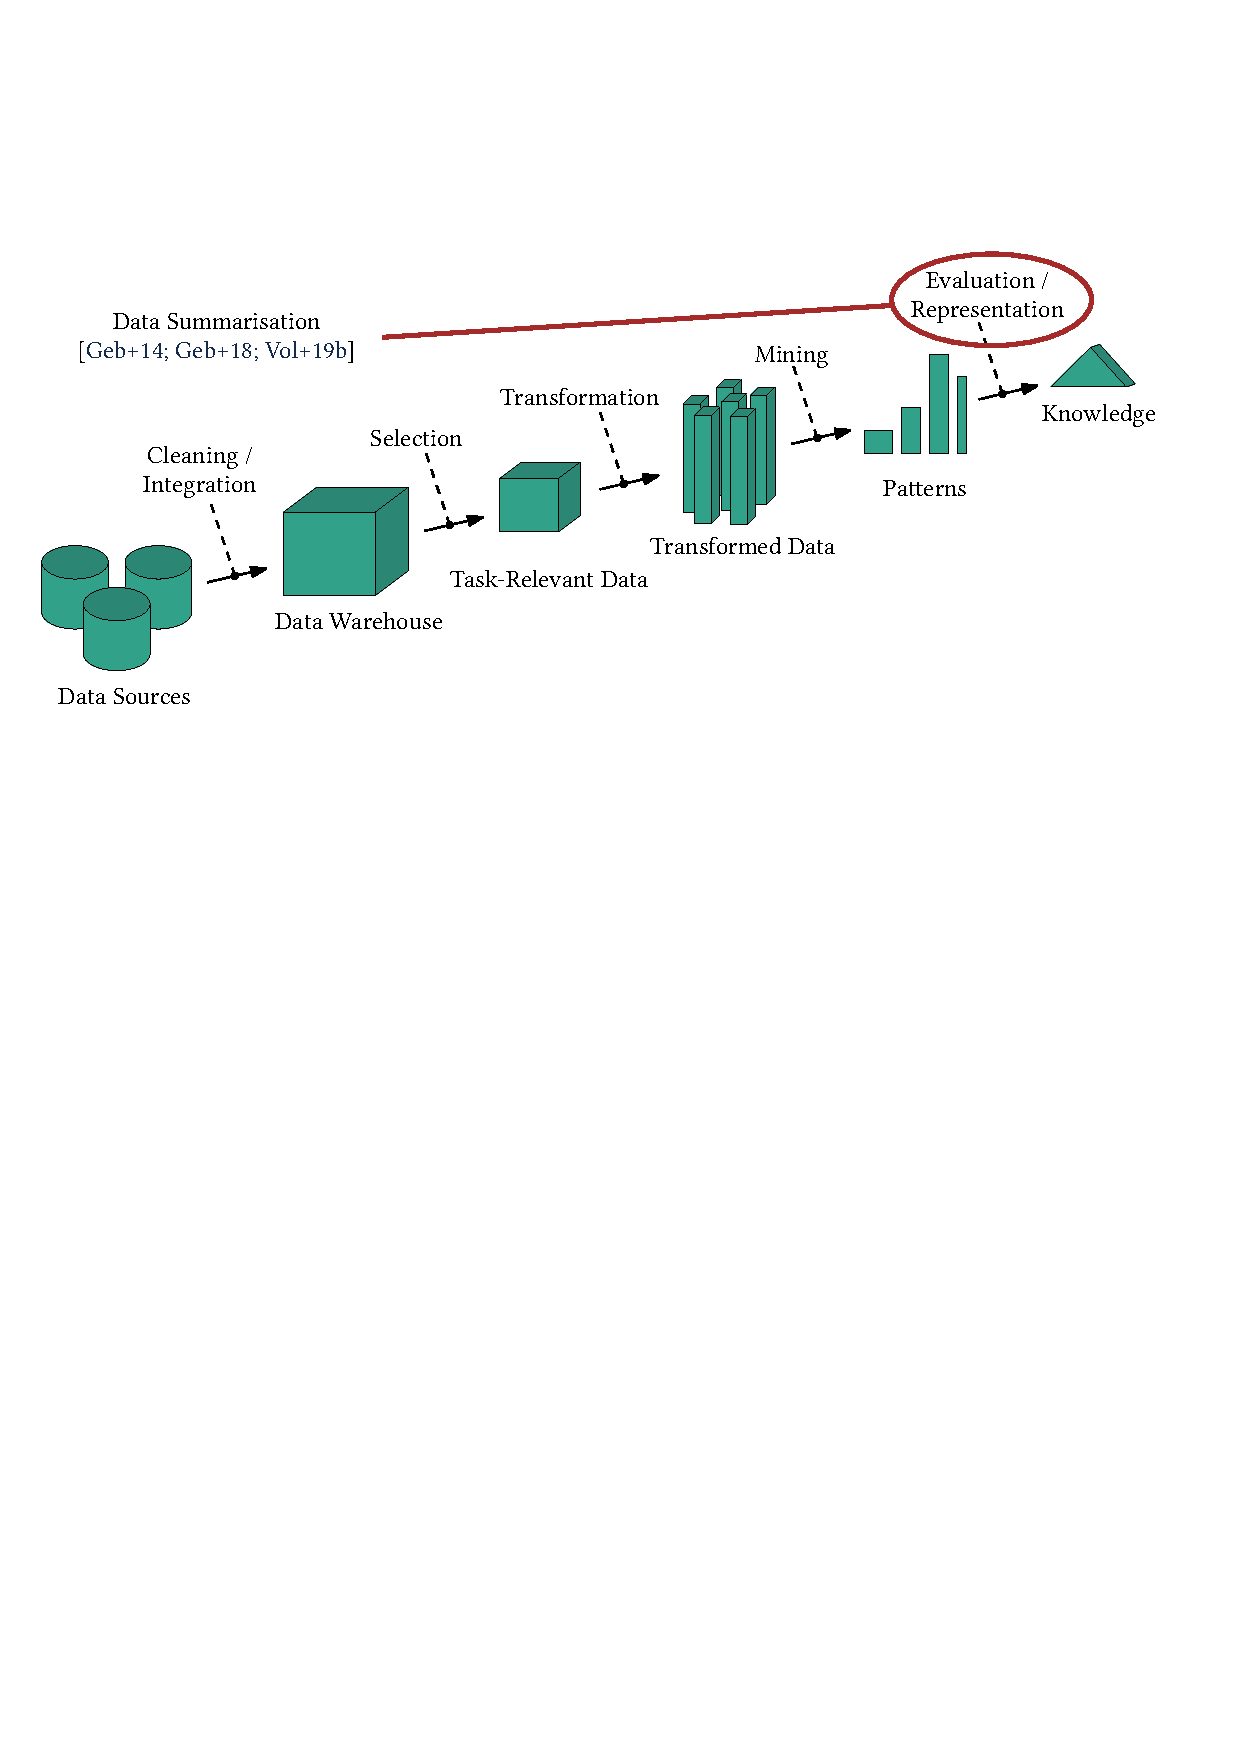
\includegraphics[width=0.98\linewidth]{figures/kdd_r5-compressed.pdf}
		\onslide<8-> 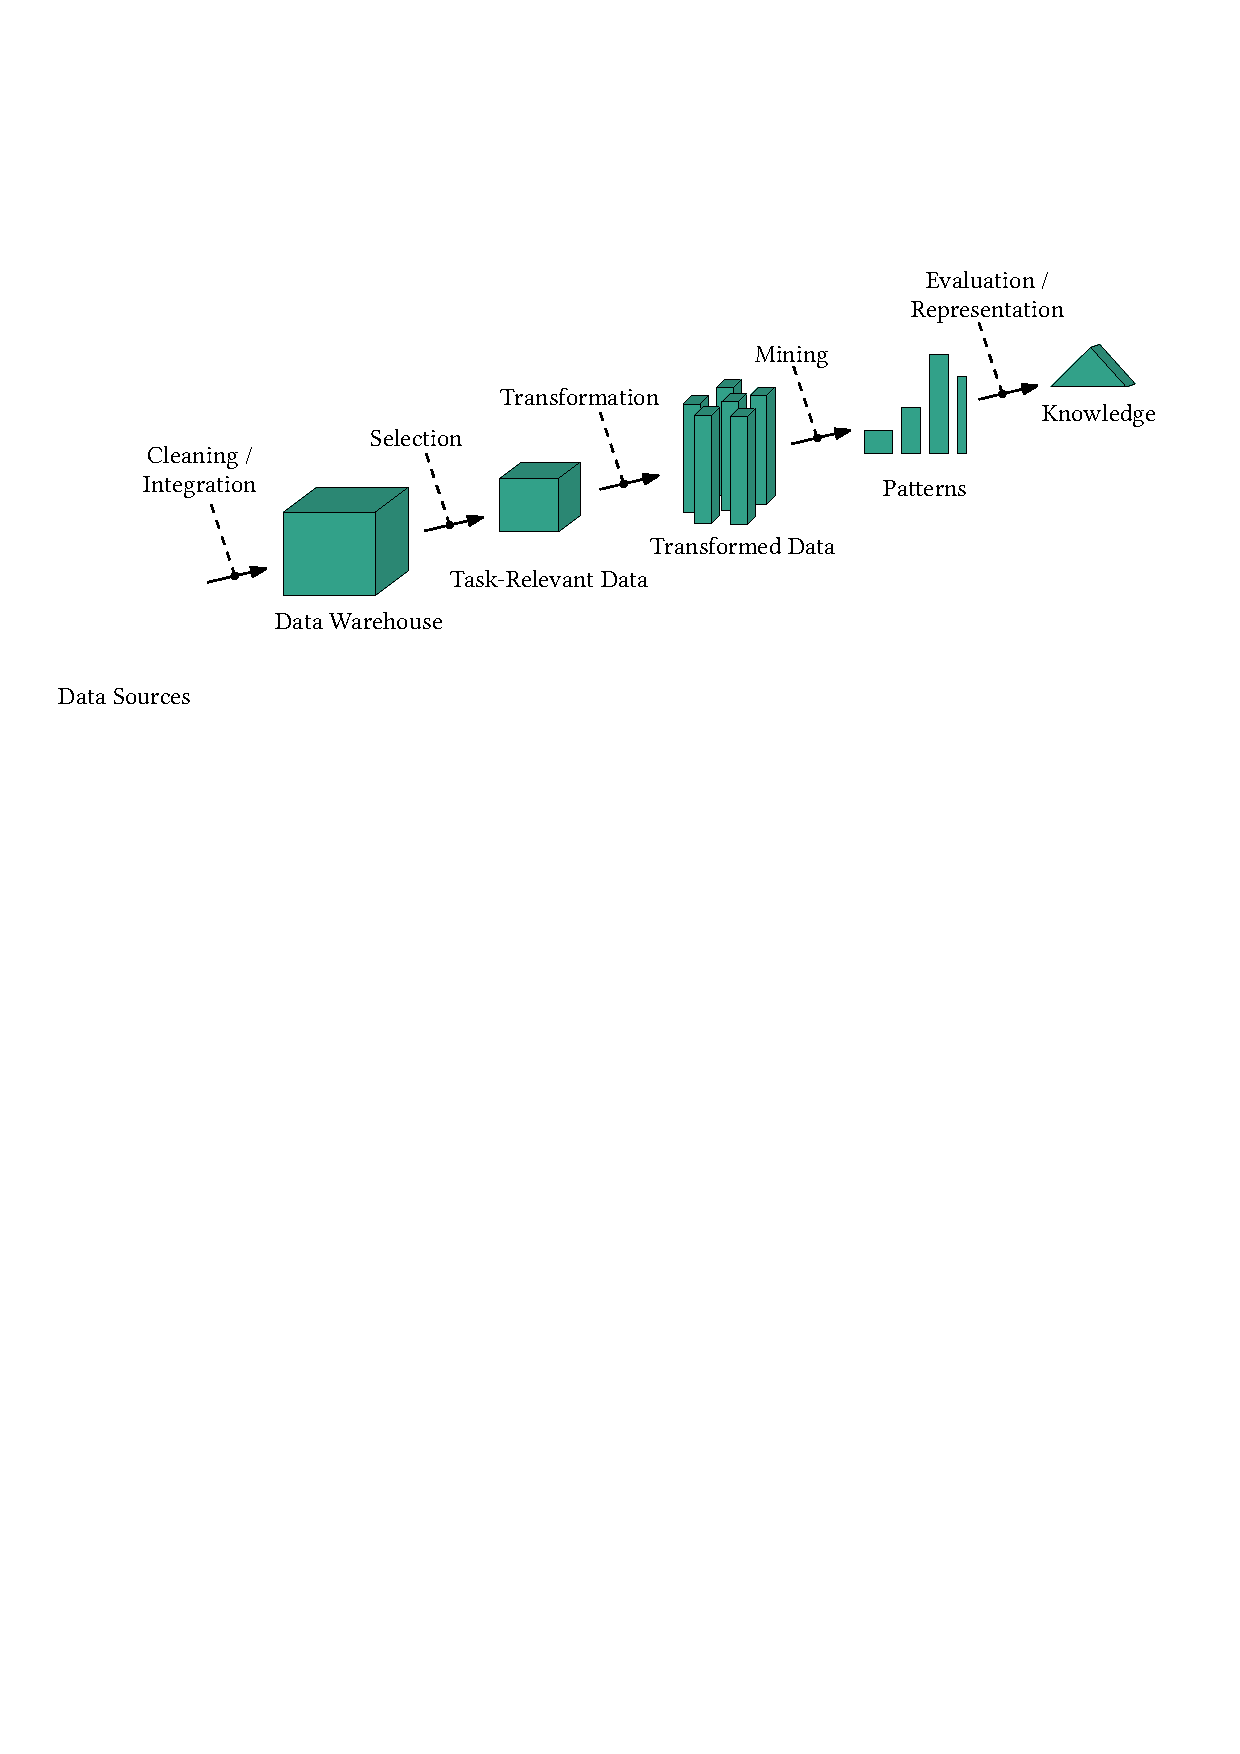
\includegraphics[width=0.98\linewidth]{figures/kdd_r6-compressed.pdf}
	\end{overprint}
\end{figure}
\pause
\pause
\pause
\pause
\pause
\pause
\begin{overprint}
	\onslide<8-> \begin{tikzpicture}[remember picture,overlay]
	\node[anchor=south east,inner sep=0pt] at ($(current page.south east)+(-10.4cm,1.8cm)$) {
		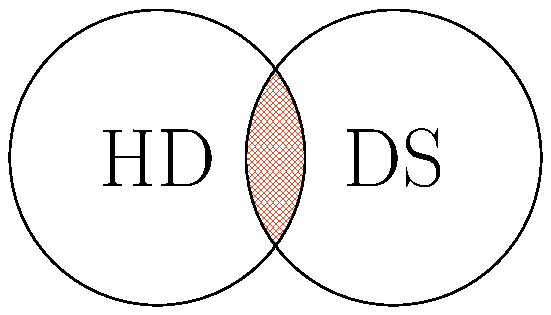
\includegraphics[angle=0, width=1.8cm]{figures/hdds_small-compressed.pdf}
	};
	\end{tikzpicture}
\end{overprint}
\vspace{-1.5cm}
\hspace{2cm} $\rightarrow$ An open problem with \textit{High-Dimensional Data Streams} !
\end{frame}
% One fundamental task of Knowledge Discovery is estimating dependency or correlation between attributes. In a nutshell, dependency, or correlation, characterises the strength of a relationship between attributes. In practice, it can *only* be estimated from empirical observations, because the underlying law is unknown. Examples of popular estimators are Pearson's or Spearman correlation, or Mutual Information. 
% From what we can see in the literature, dependency estimation is helpful at virtually any stage of the KDD pipeline: 
% A subfield, known as Exploratory Data Mining, aims to reveal structure in the data, e.g., artefacts and inconsistencies that one should clean. To do that, dependency estimators are an essential tool. 
% Then, feature selection methods heavily rely on dependency estimators to filter out the attributes which are irrelevant for the task at hand.
% Data Transformation is also known as Feature Engineering. Dependency estimators often are considered as "features" that one can to improve the results of downstream analysis. 
% Numerous Data Mining algorithms, such as clustering or outlier detection algorithms intrinsically rely on dependency estimation.
% Finally, dependency estimation is also helpful for pattern evaluation and representation. For example, several existing works leverage mutual information to represent rules learned from data.  
% However, there are to our knowledge no dependency estimation methods suitable for high-dimensional data streams. 

\begin{frame}{Bioliq\textsuperscript{\textregistered}: The pyrolysis as a HD-DS}

\begin{figure}
	\begin{overprint}
		\onslide<1-> 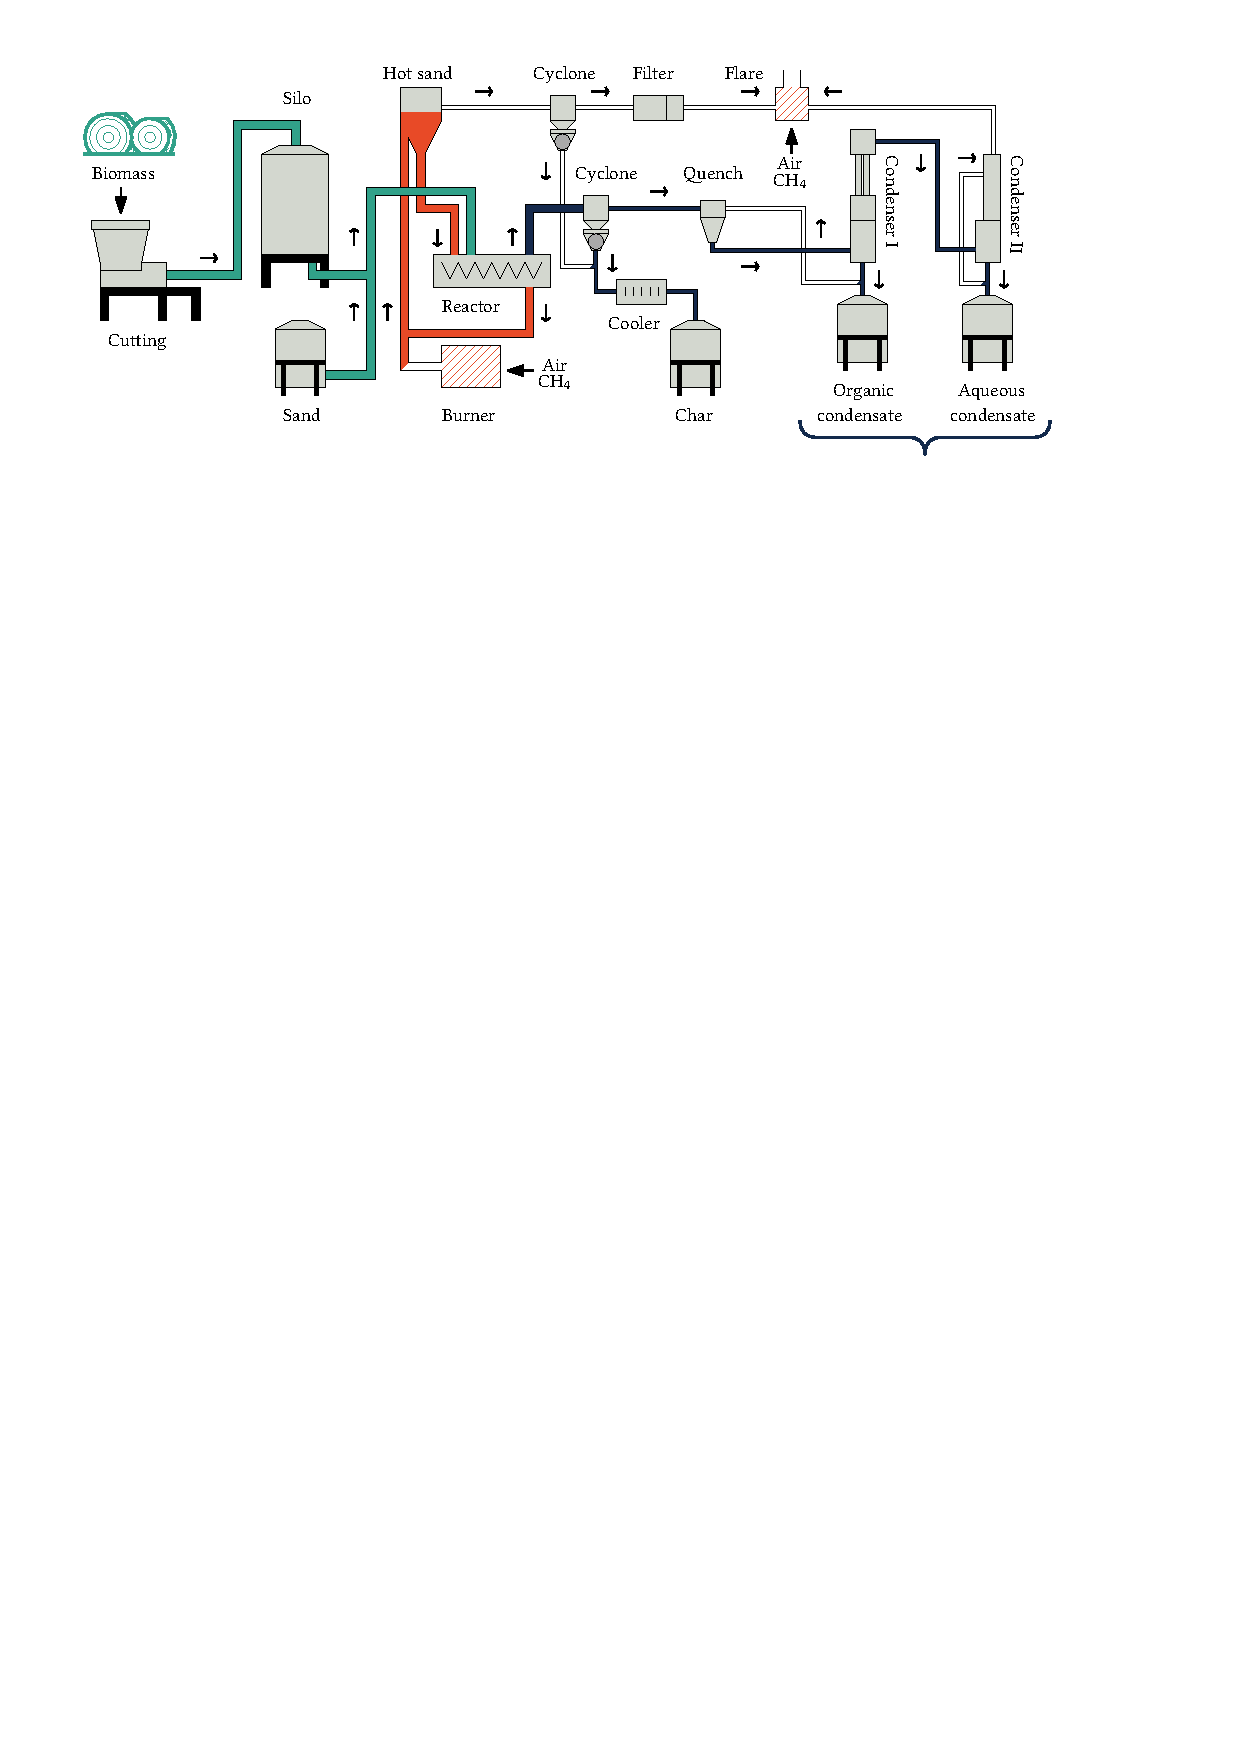
\includegraphics[width=1.0 \linewidth]{figures/bioliq_schematics_2-compressed.pdf}
	\end{overprint}
\caption*{Simplified schematics of Bioliq's Pyrolysis}
\end{figure}
\begin{overprint}
	\onslide<1-> \begin{tikzpicture}[remember picture,overlay]
	\node[anchor=south east,inner sep=0pt] at ($(current page.south east)+(-1.7cm,1.8cm)$) {
		
\includegraphics[angle=0, width=1cm]{figures/fuel-compressed.pdf}
	};
	\end{tikzpicture}
\end{overprint}
\pause
\vspace{-1cm}
\begin{itemize}
	\item $>$ 400 sensors, continuously measured $\rightarrow$ HD-DS
	\pause
	\item Data Mining may help to analyse the pyrolysis process
\end{itemize}
\end{frame}
% In my dissertation, I illustrate and motivate my results against a real-world use case: the Bioliq power plant. In a nutshell, the goal of Bioliq project is to develop the process chain for producing fuel from biomass at an industrial scale. One fundamental step of the process is the so-called "fast pyrolysis", and here you can see a simplified representation of this process, which takes place in a pilot plant at KIT campus north. 

% The fast pyrolysis is still experimental and relatively difficult to control and maintain over time. Based on data, we might improve our knowledge about the pyrolysis process. The plant is equipped with hundreds of sensors and data is continuously collected, so this a suitable example of a high-dimensional stream.  

%\subsection{Contributions}
% Based on these observations, I defined three research questions, around which my thesis gravitates. The first question is how to estimate dependency in high-dimensional data streams efficiently and effectively. The reason is that existing methods are not satisfying in that setting, as we will see later. Then, once we can estimate dependency, how can one keep track of the evolution of such estimates (or virtually any statistics) in high-dimensional data streams? Finally, we can learn or how can we leverage from such new monitoring and estimation techniques. I am thinking about more concrete patterns for end-users, such as anomalies, in this context. 

% Those questions form the three pillars of my thesis, which we may find in its title and its structure as well: 

\begin{frame}{Our Contributions}

are organised around 3 research questions: 
\begin{figure}
	\begin{overprint}
		\onslide<1> 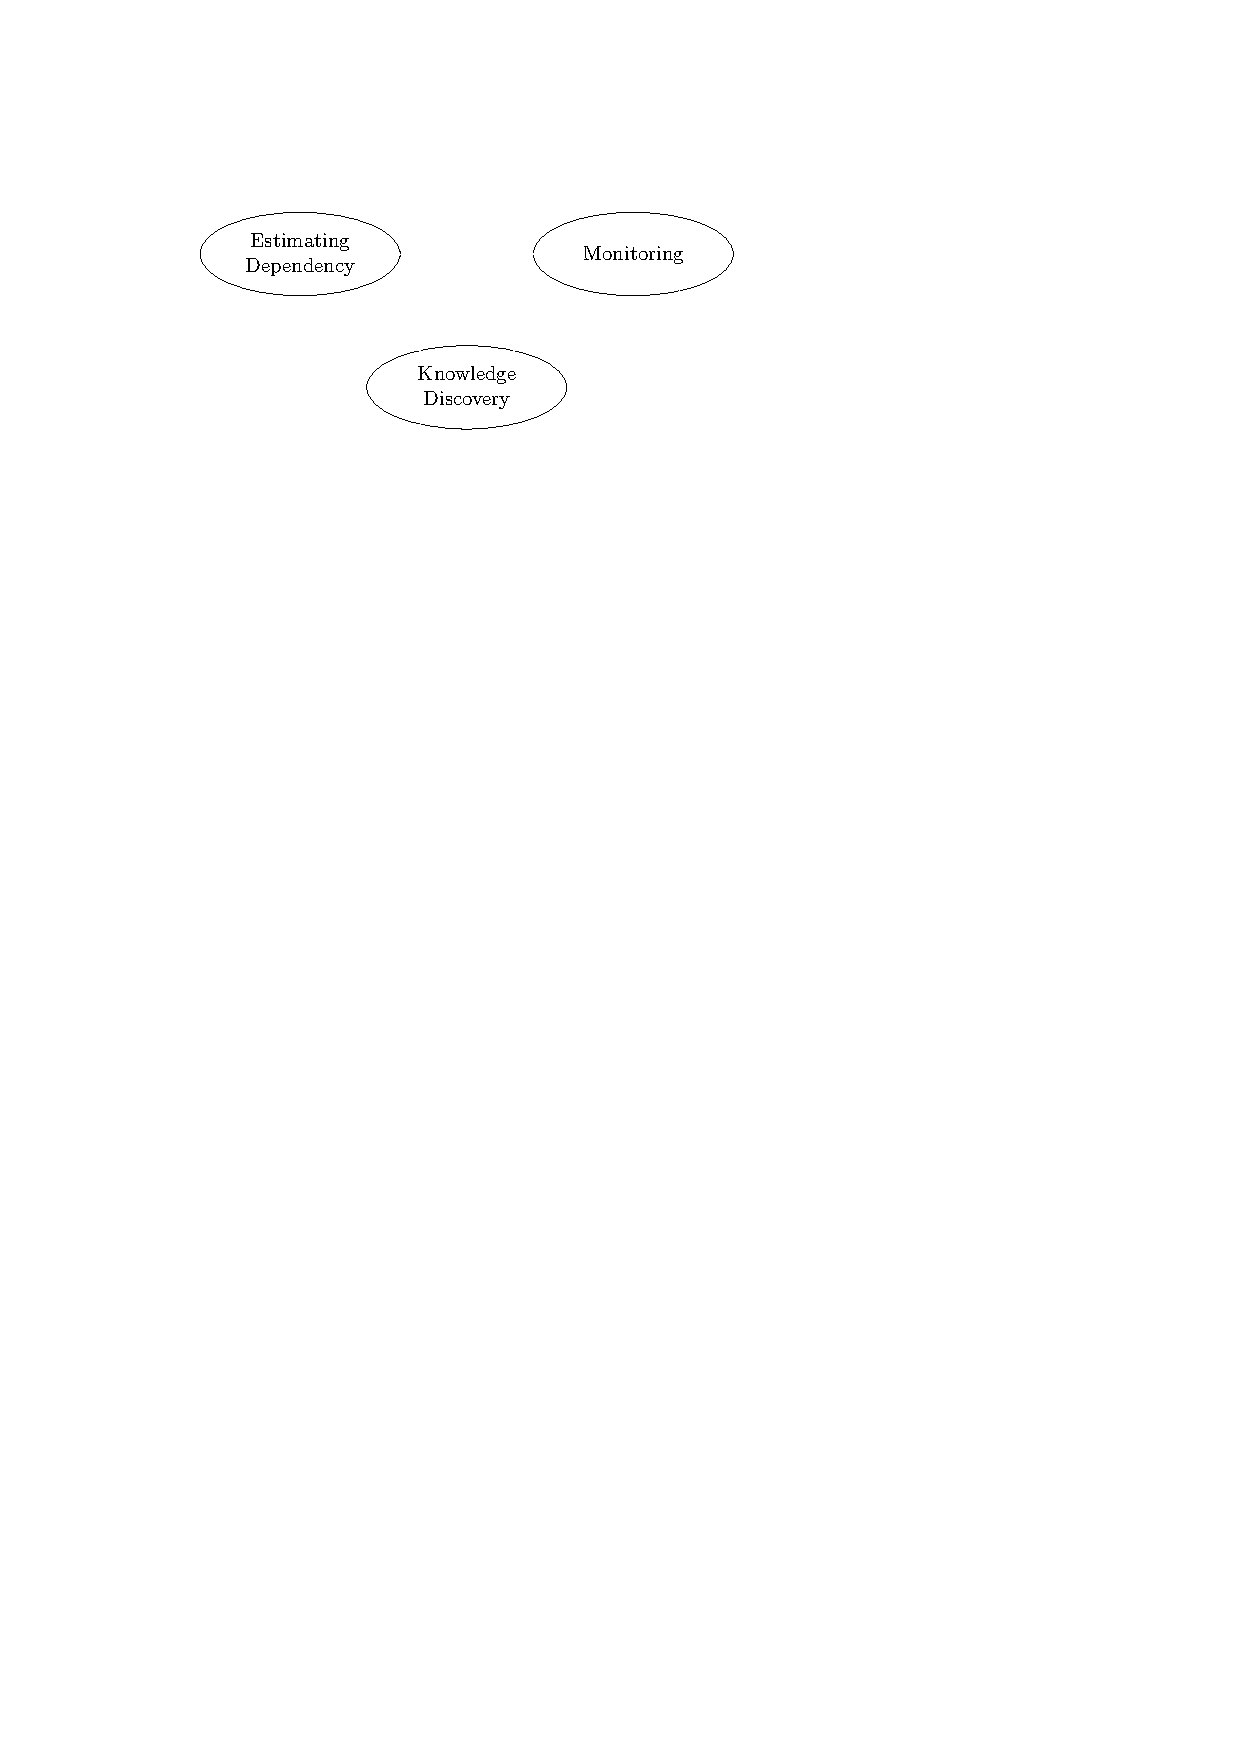
\includegraphics[width=1.0 \linewidth]{figures/outline_c_0-compressed.pdf}
		\onslide<2> 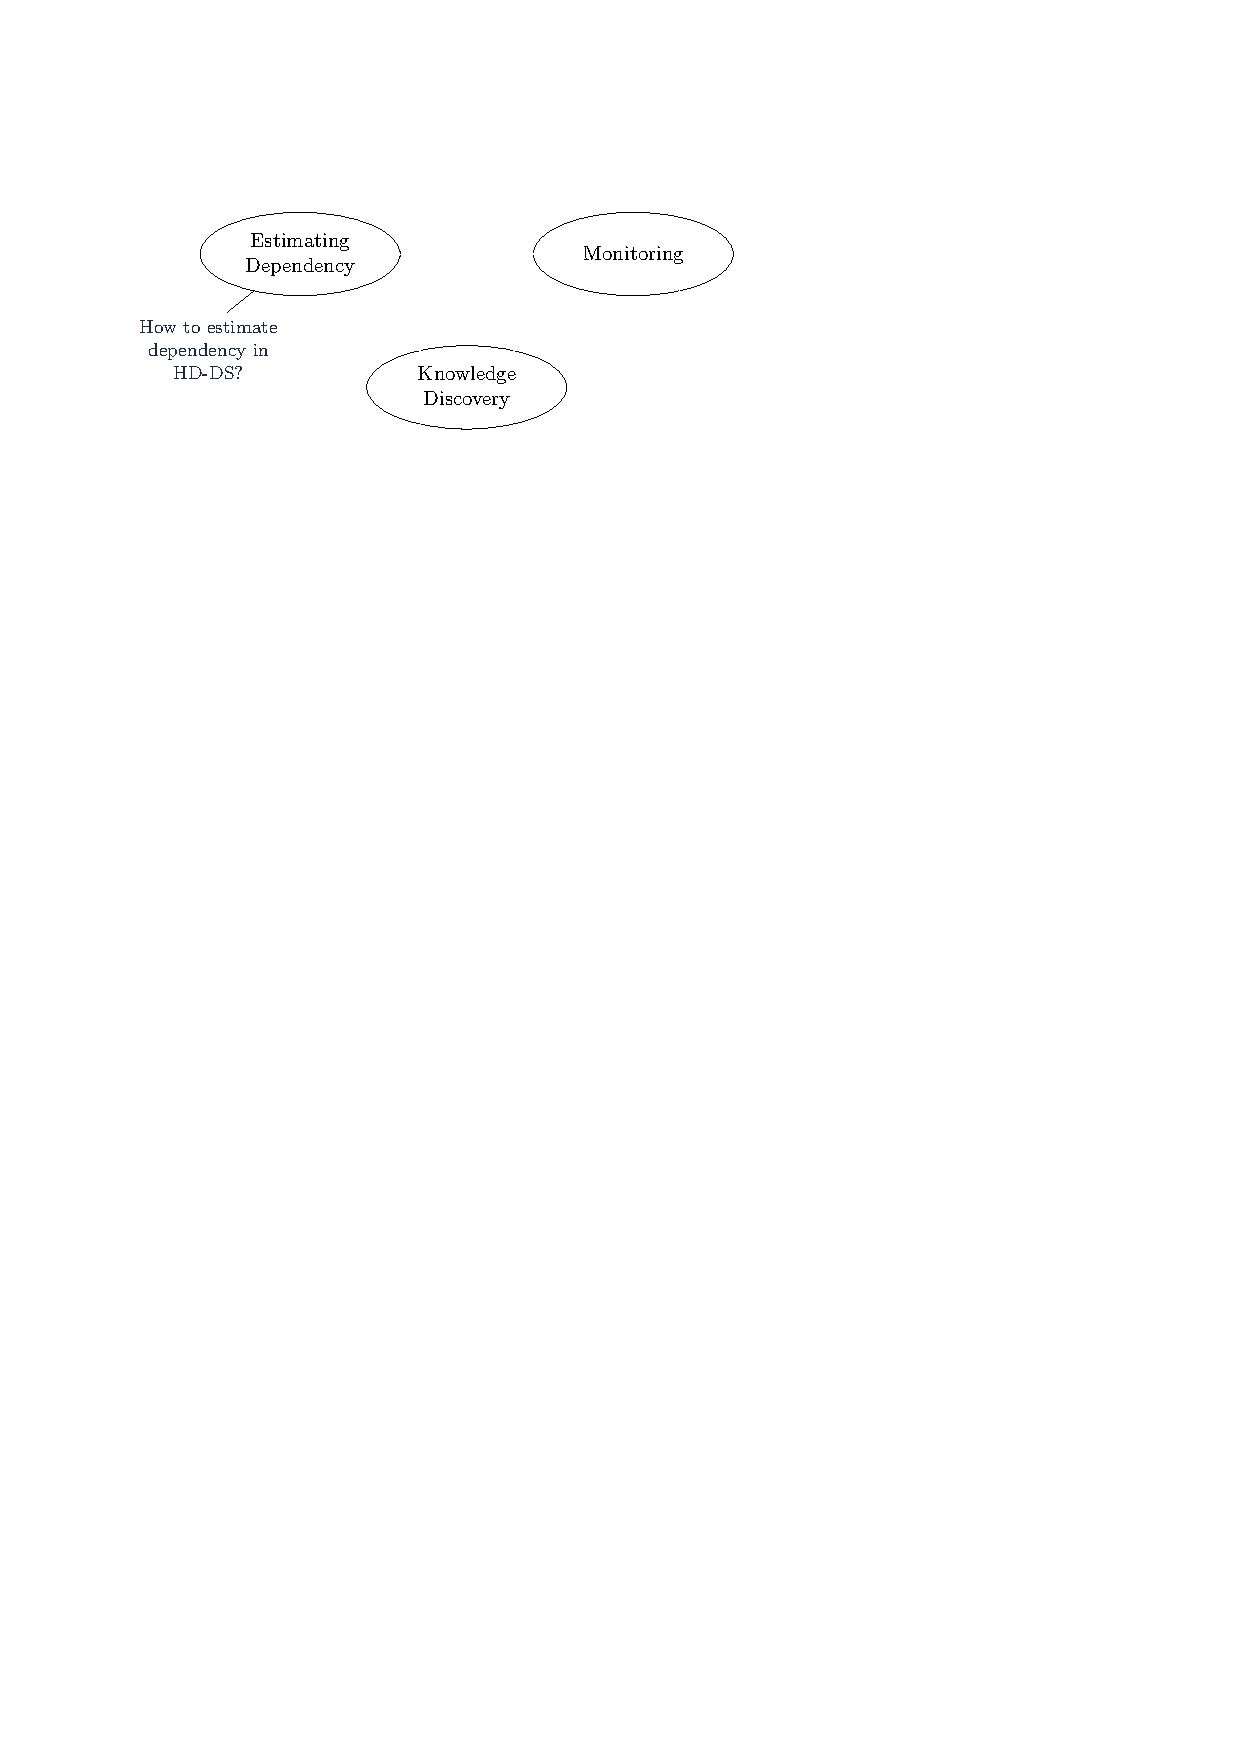
\includegraphics[width=1.0 \linewidth]{figures/outline_c_1-compressed.pdf}
		\onslide<3> 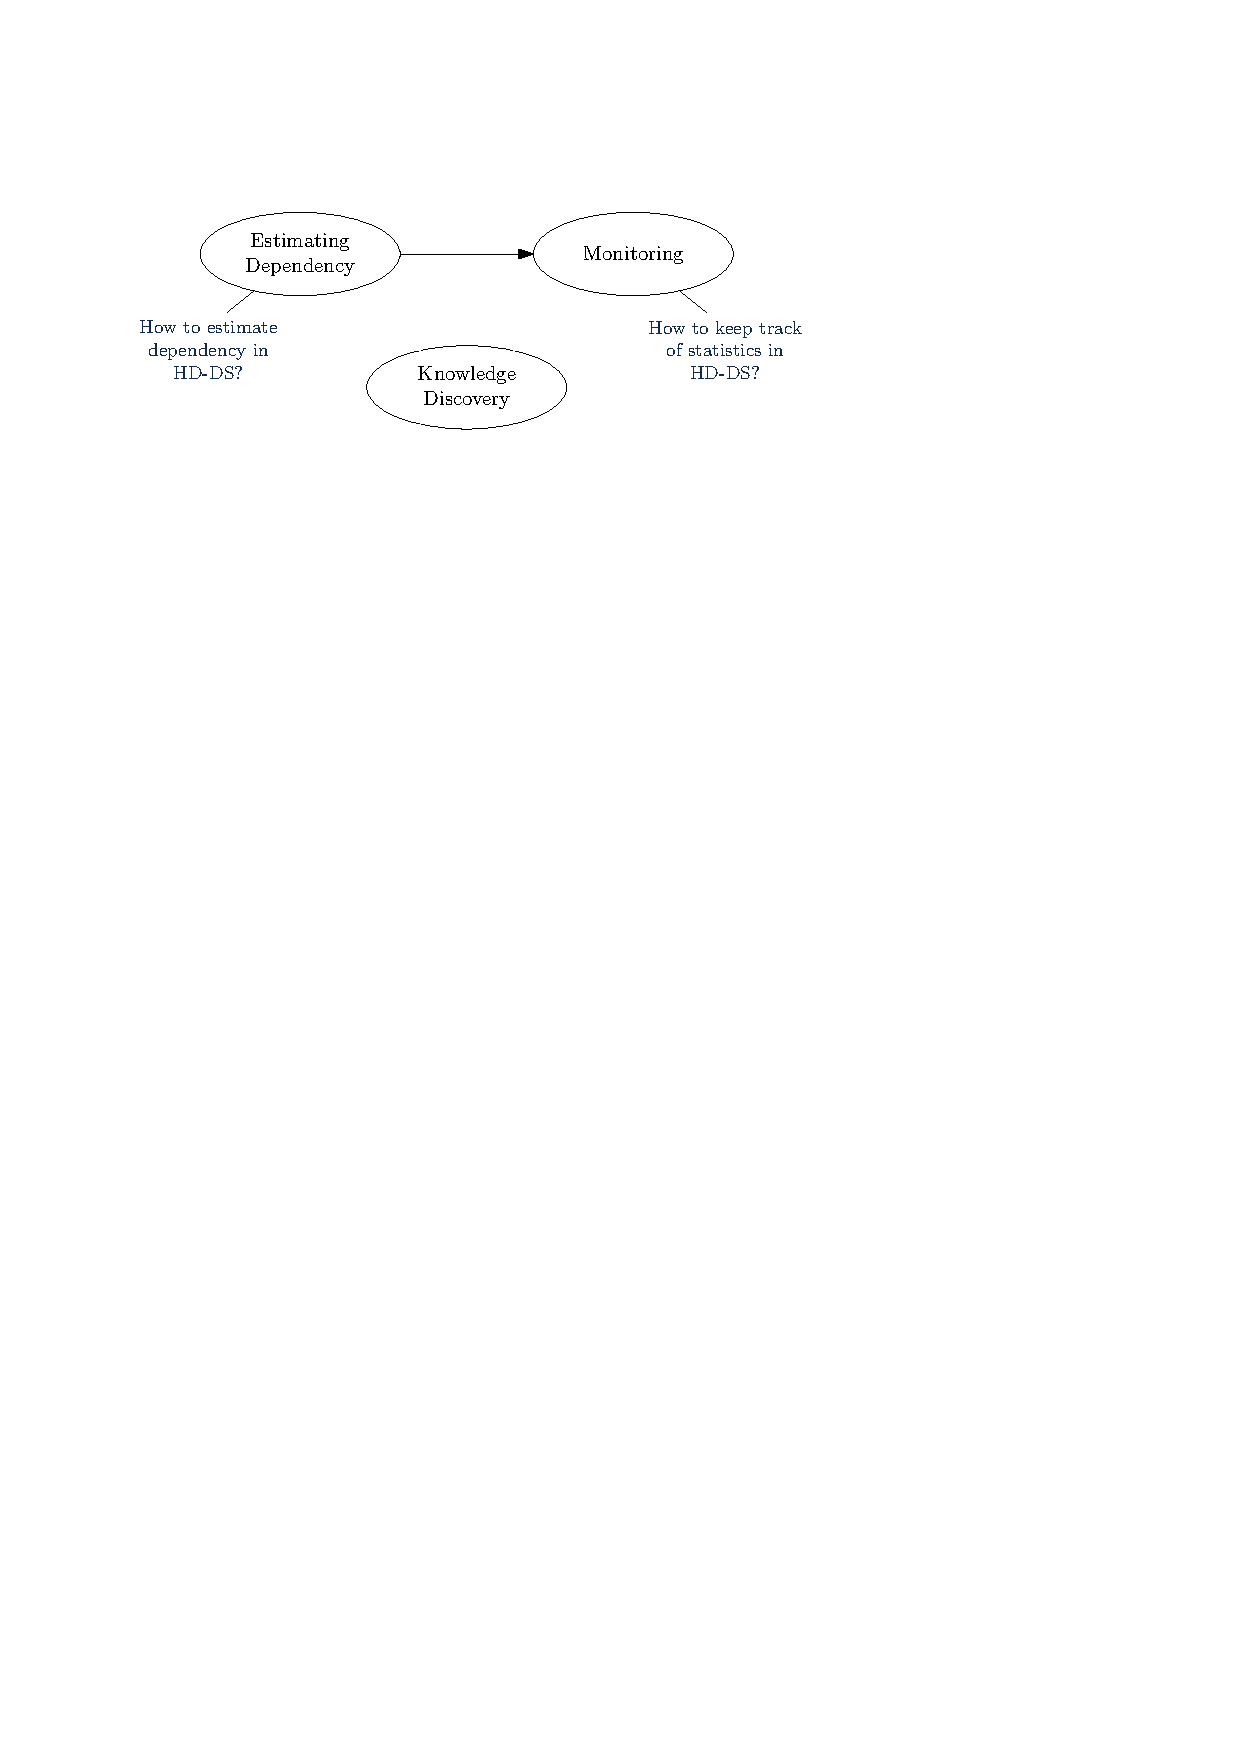
\includegraphics[width=1.0 \linewidth]{figures/outline_c_2-compressed.pdf}
		\onslide<4> 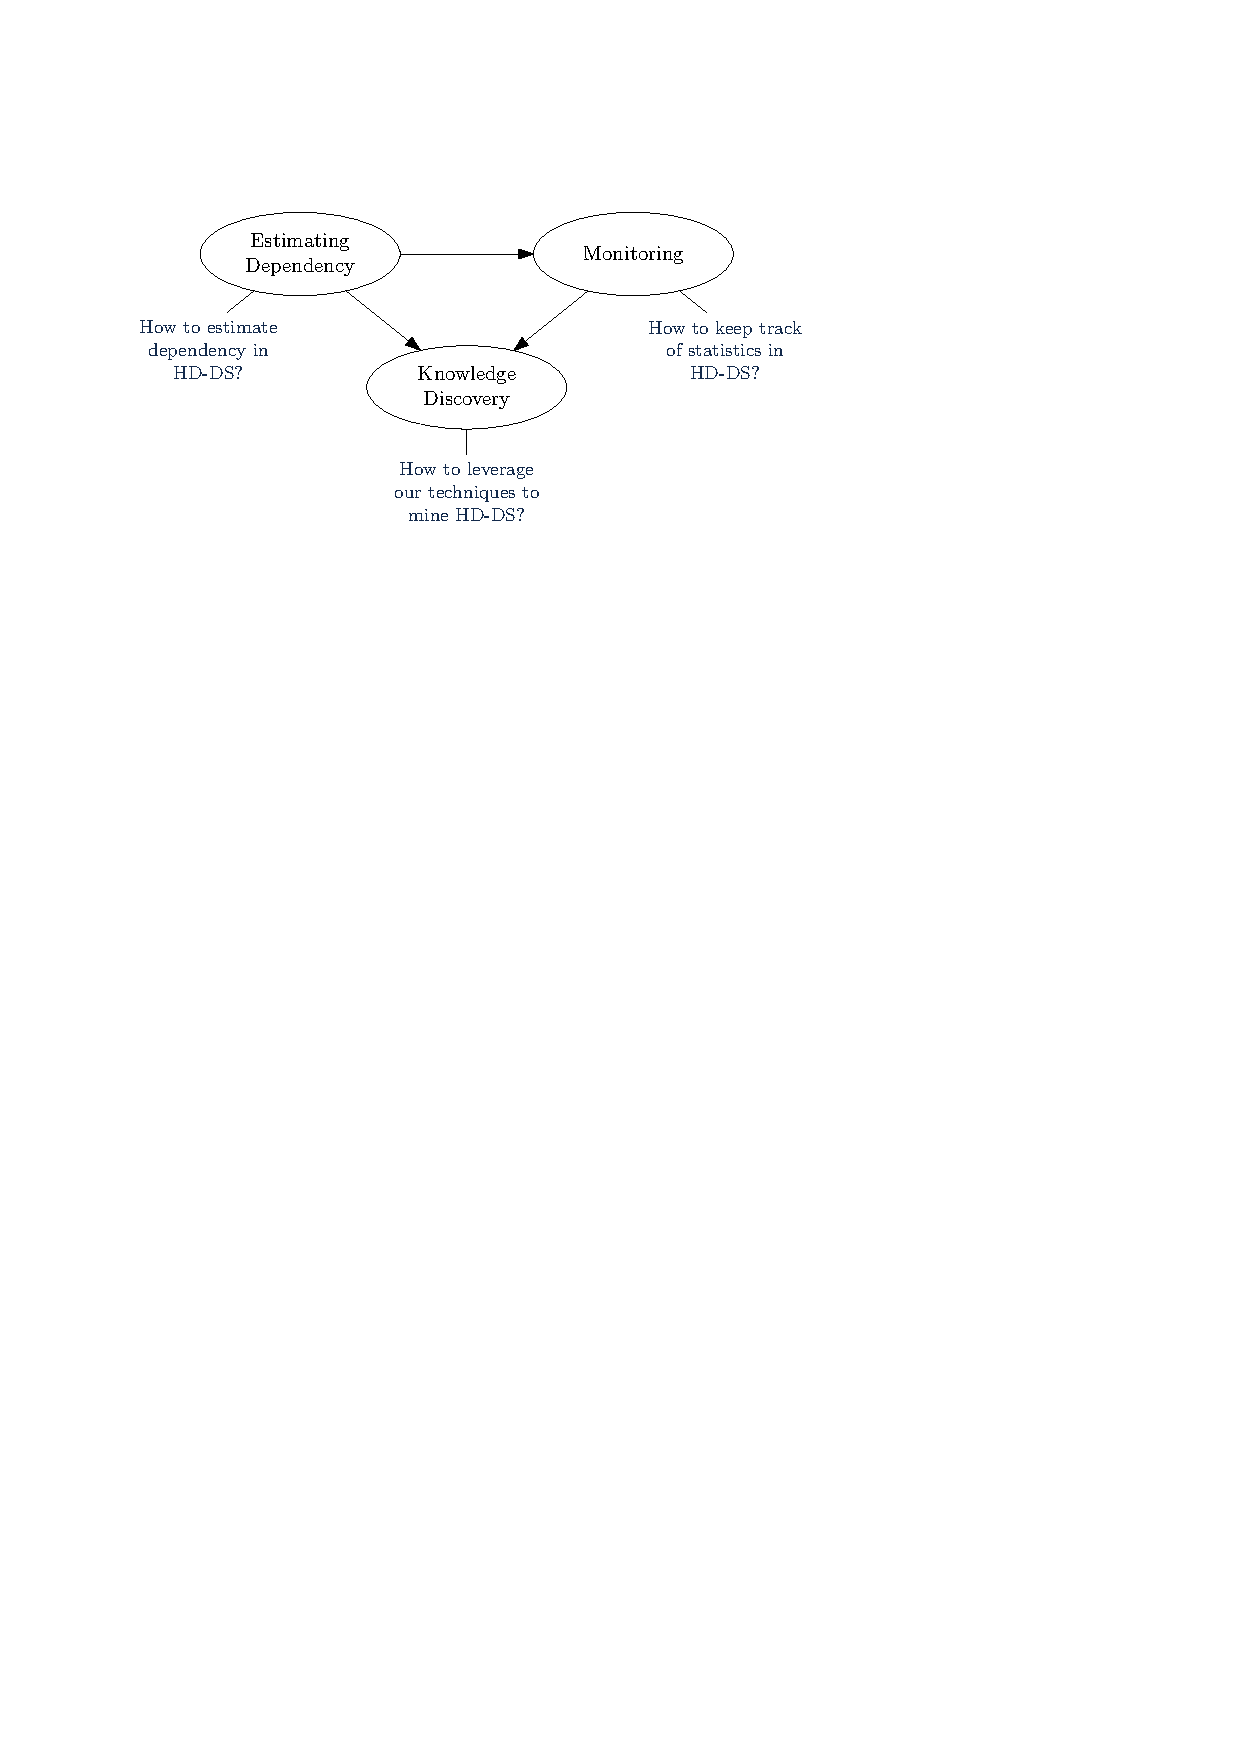
\includegraphics[width=1.0 \linewidth]{figures/outline_c_3-compressed.pdf}
		\onslide<5> 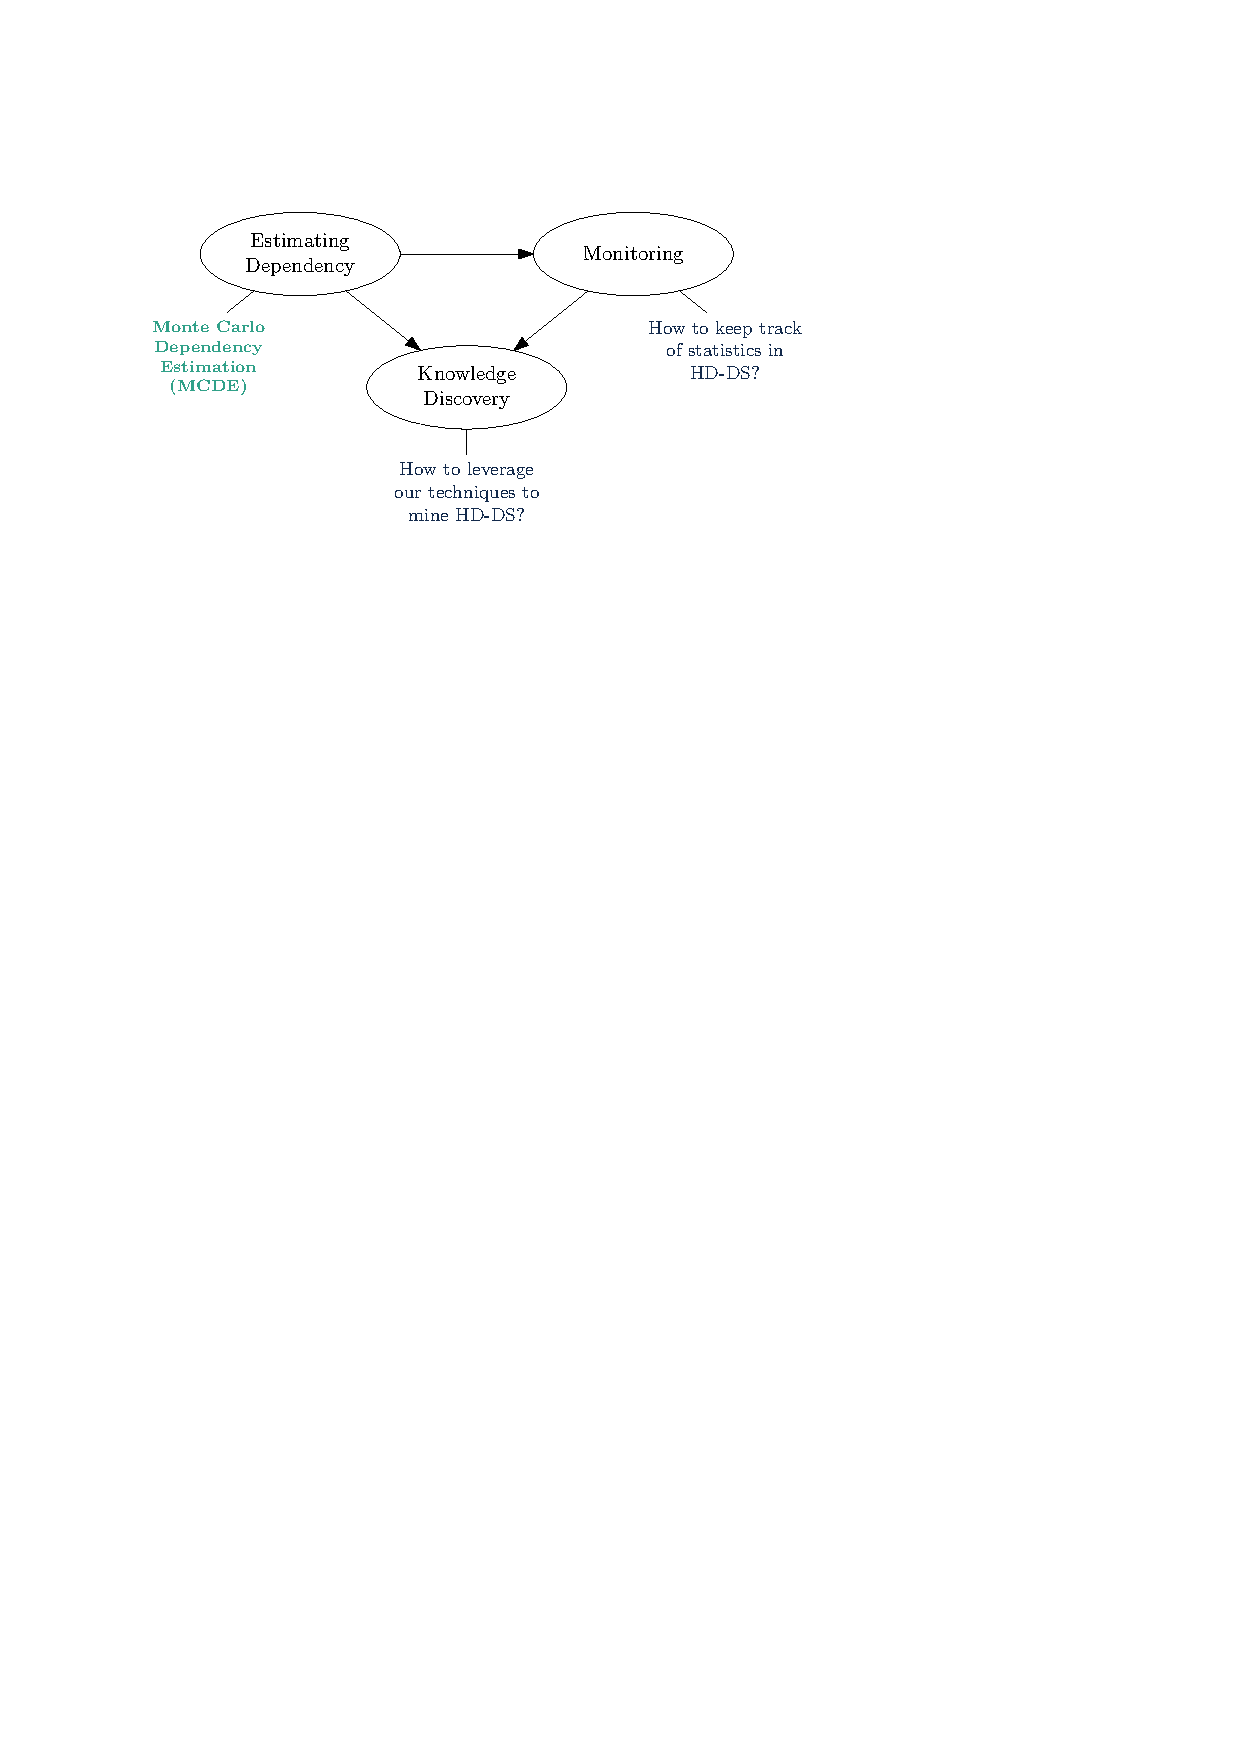
\includegraphics[width=1.0 \linewidth]{figures/outline_c_4-compressed.pdf}
		\onslide<6> 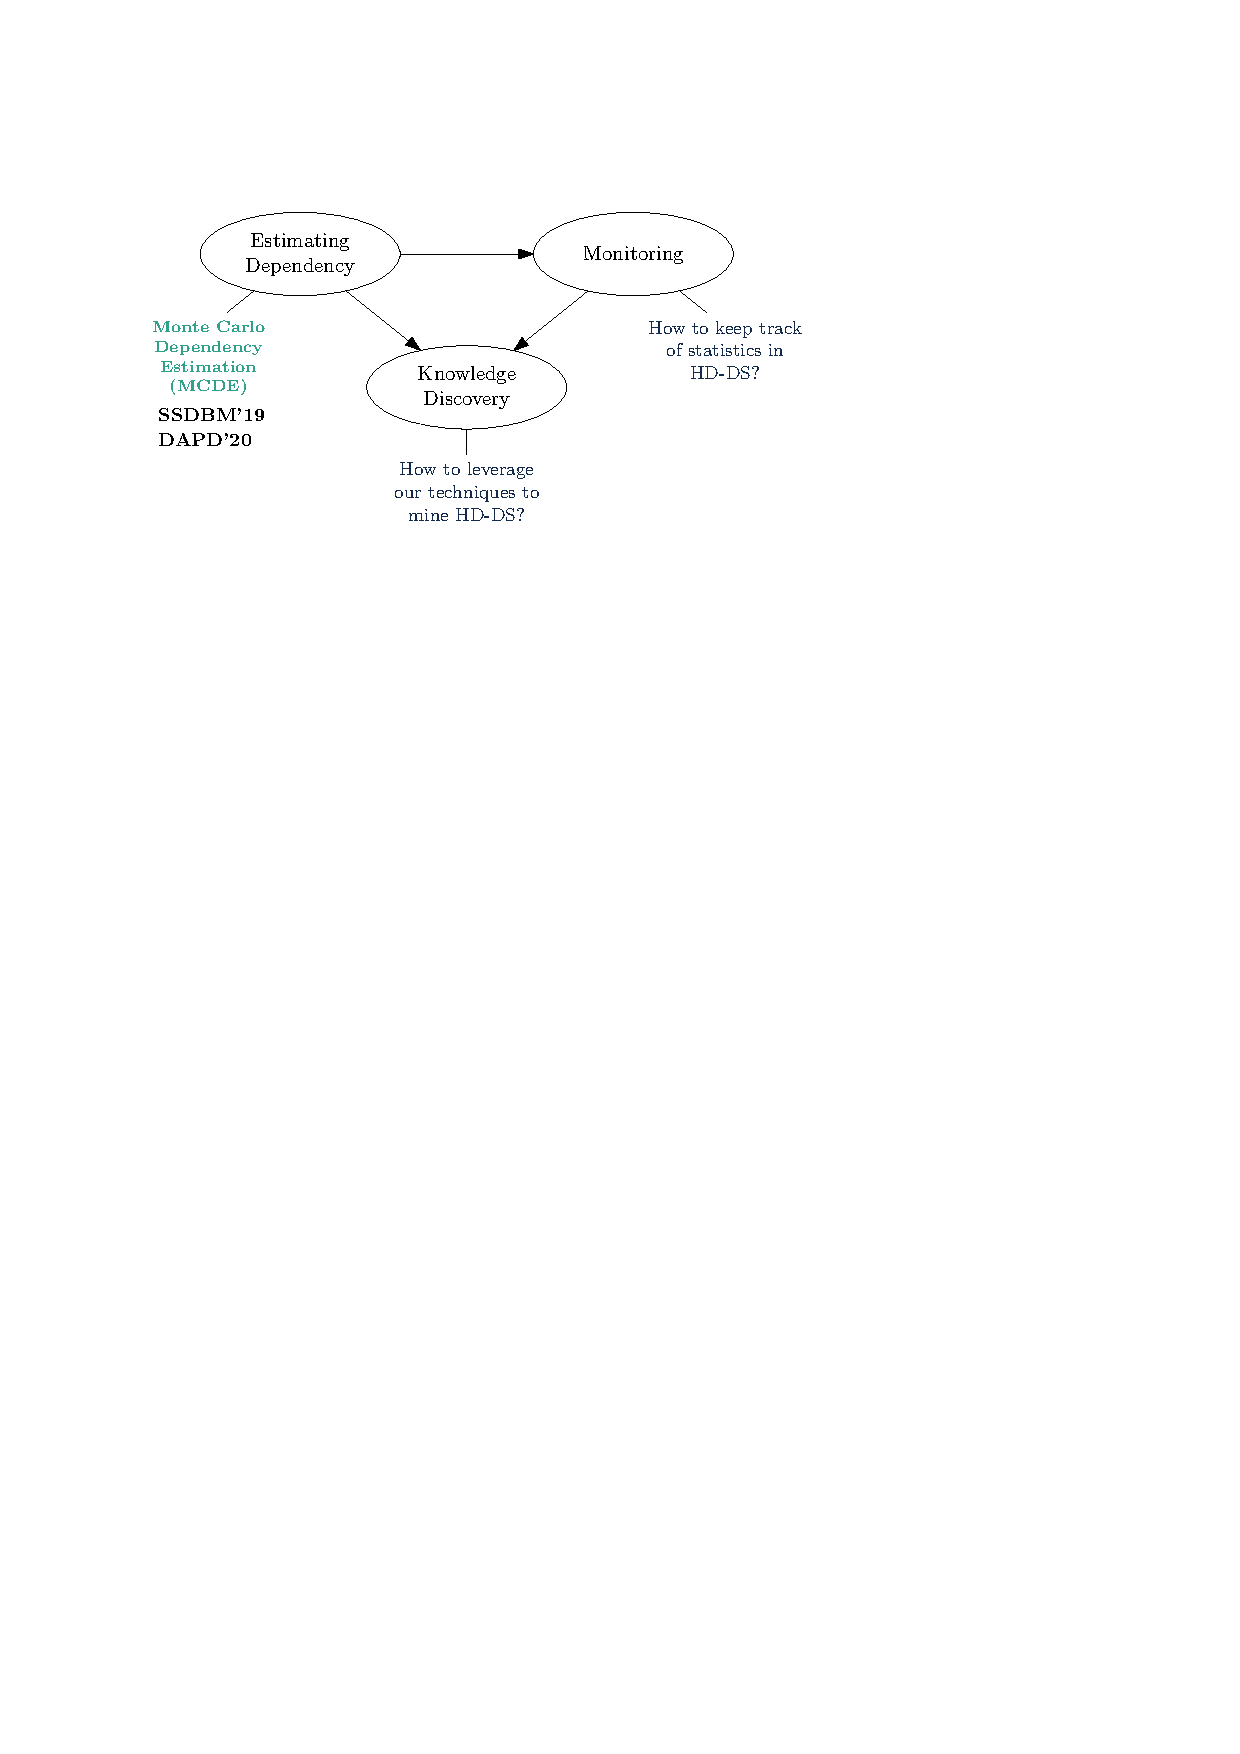
\includegraphics[width=1.0 \linewidth]{figures/outline_c_5-compressed.pdf}
		\onslide<7> 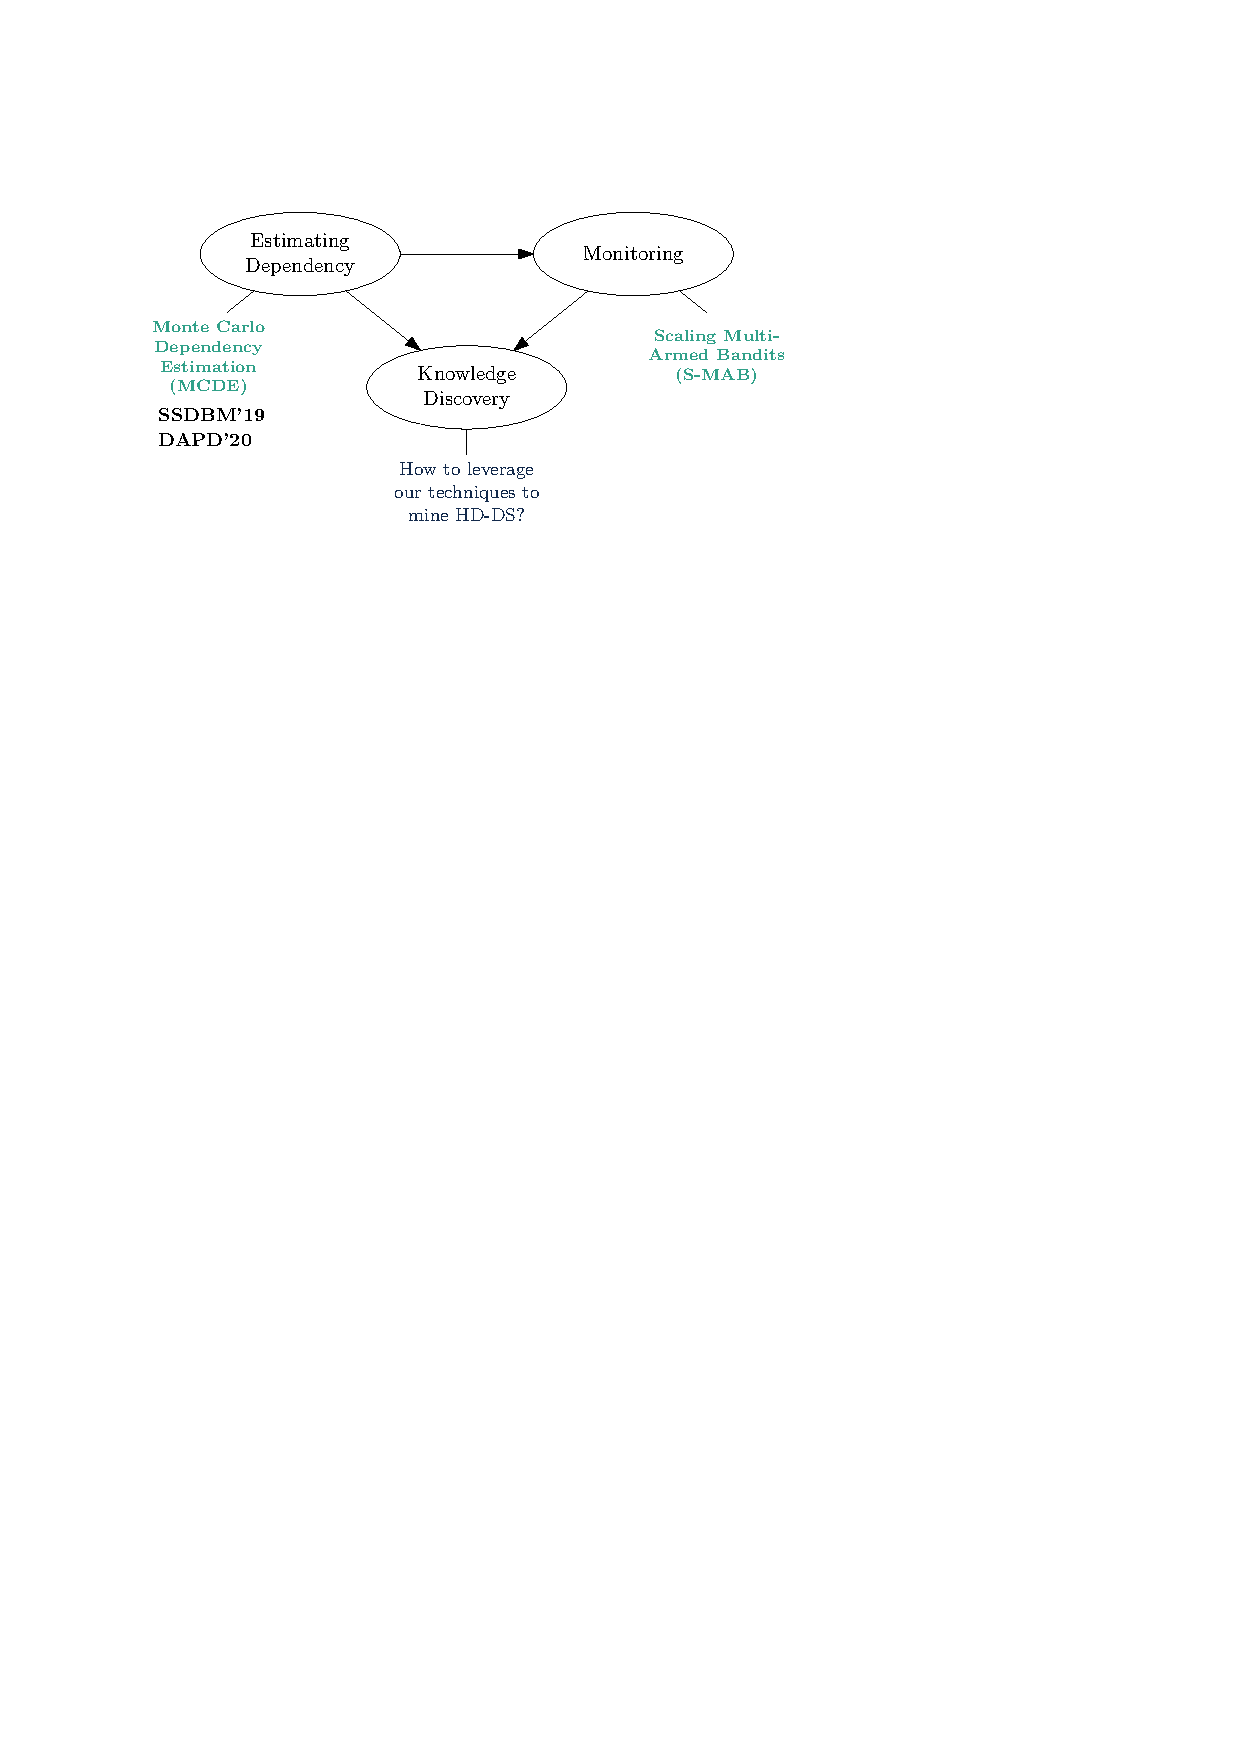
\includegraphics[width=1.0 \linewidth]{figures/outline_c_6-compressed.pdf}
		\onslide<8> 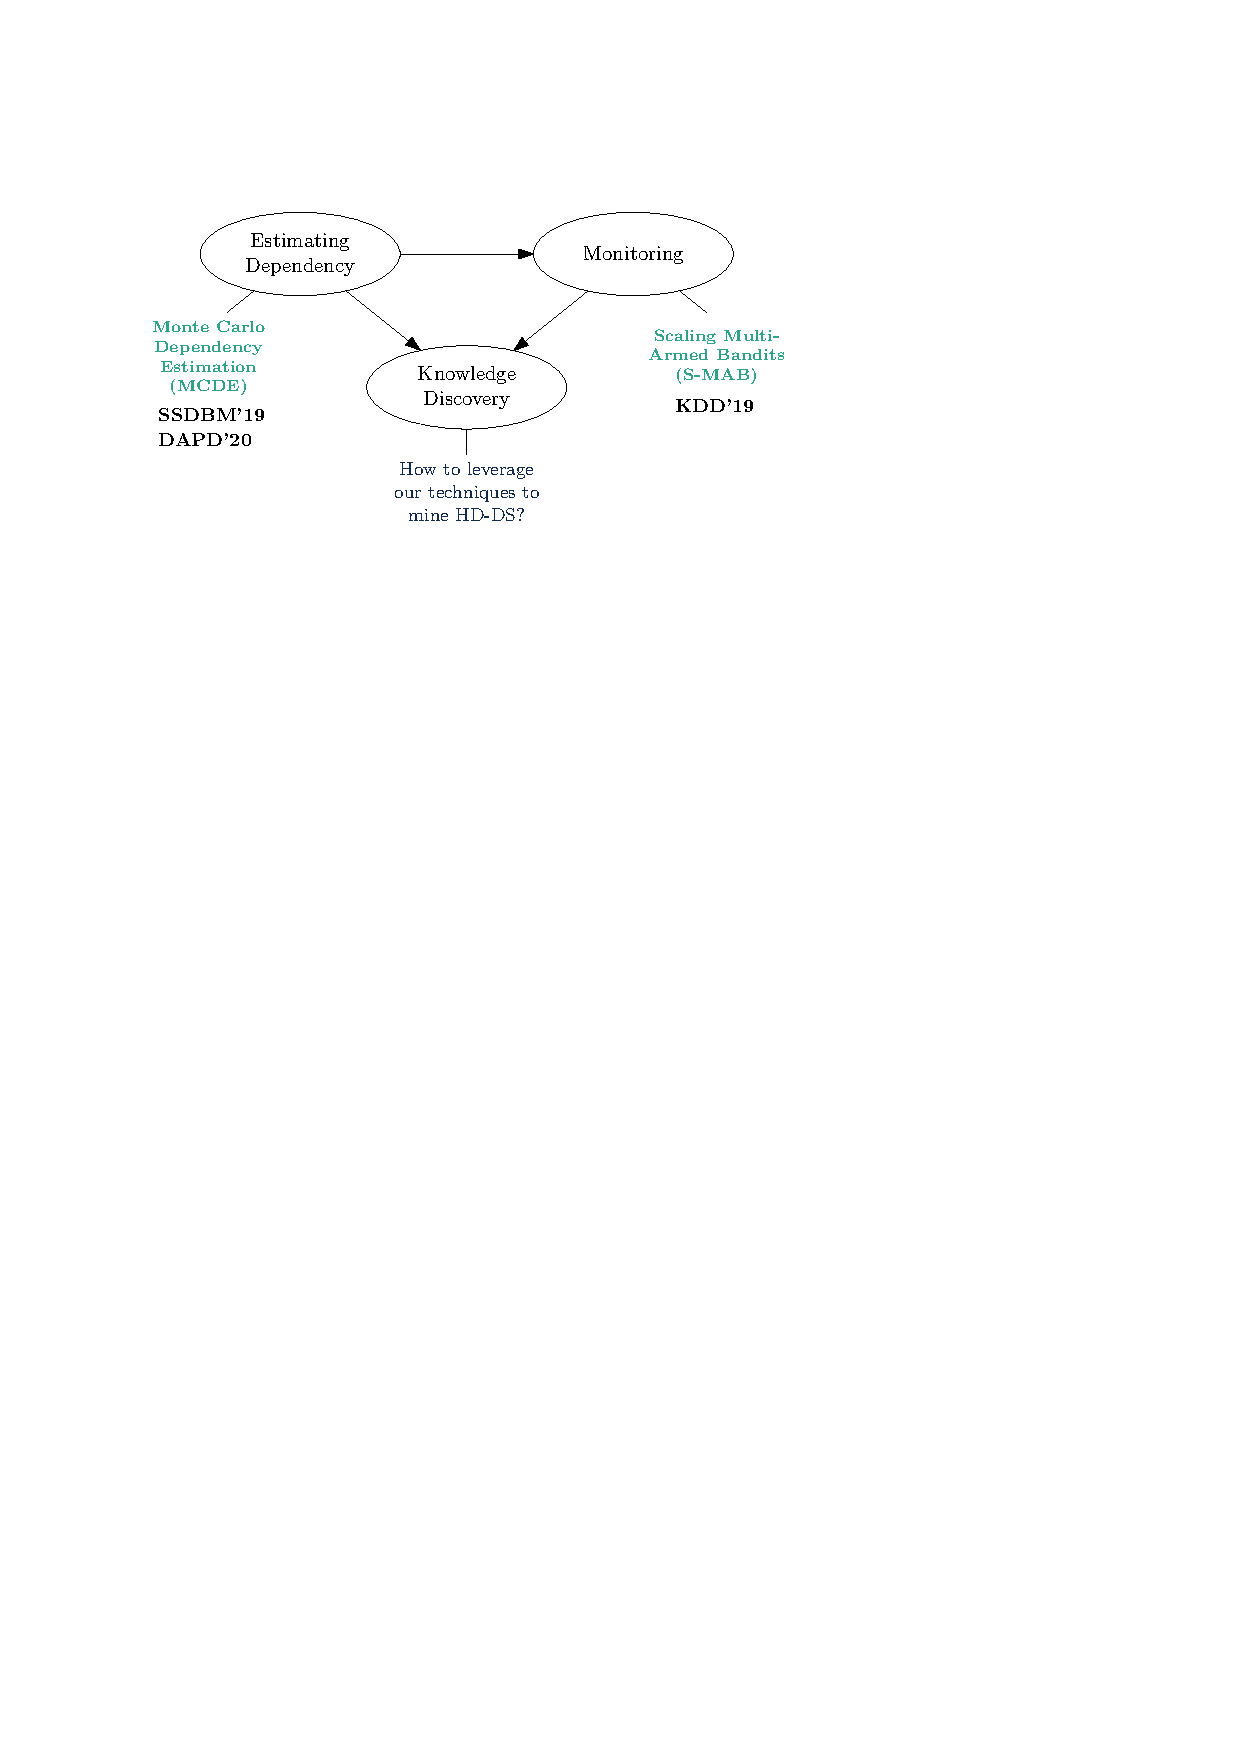
\includegraphics[width=1.0 \linewidth]{figures/outline_c_7-compressed.pdf}
		\onslide<9-> 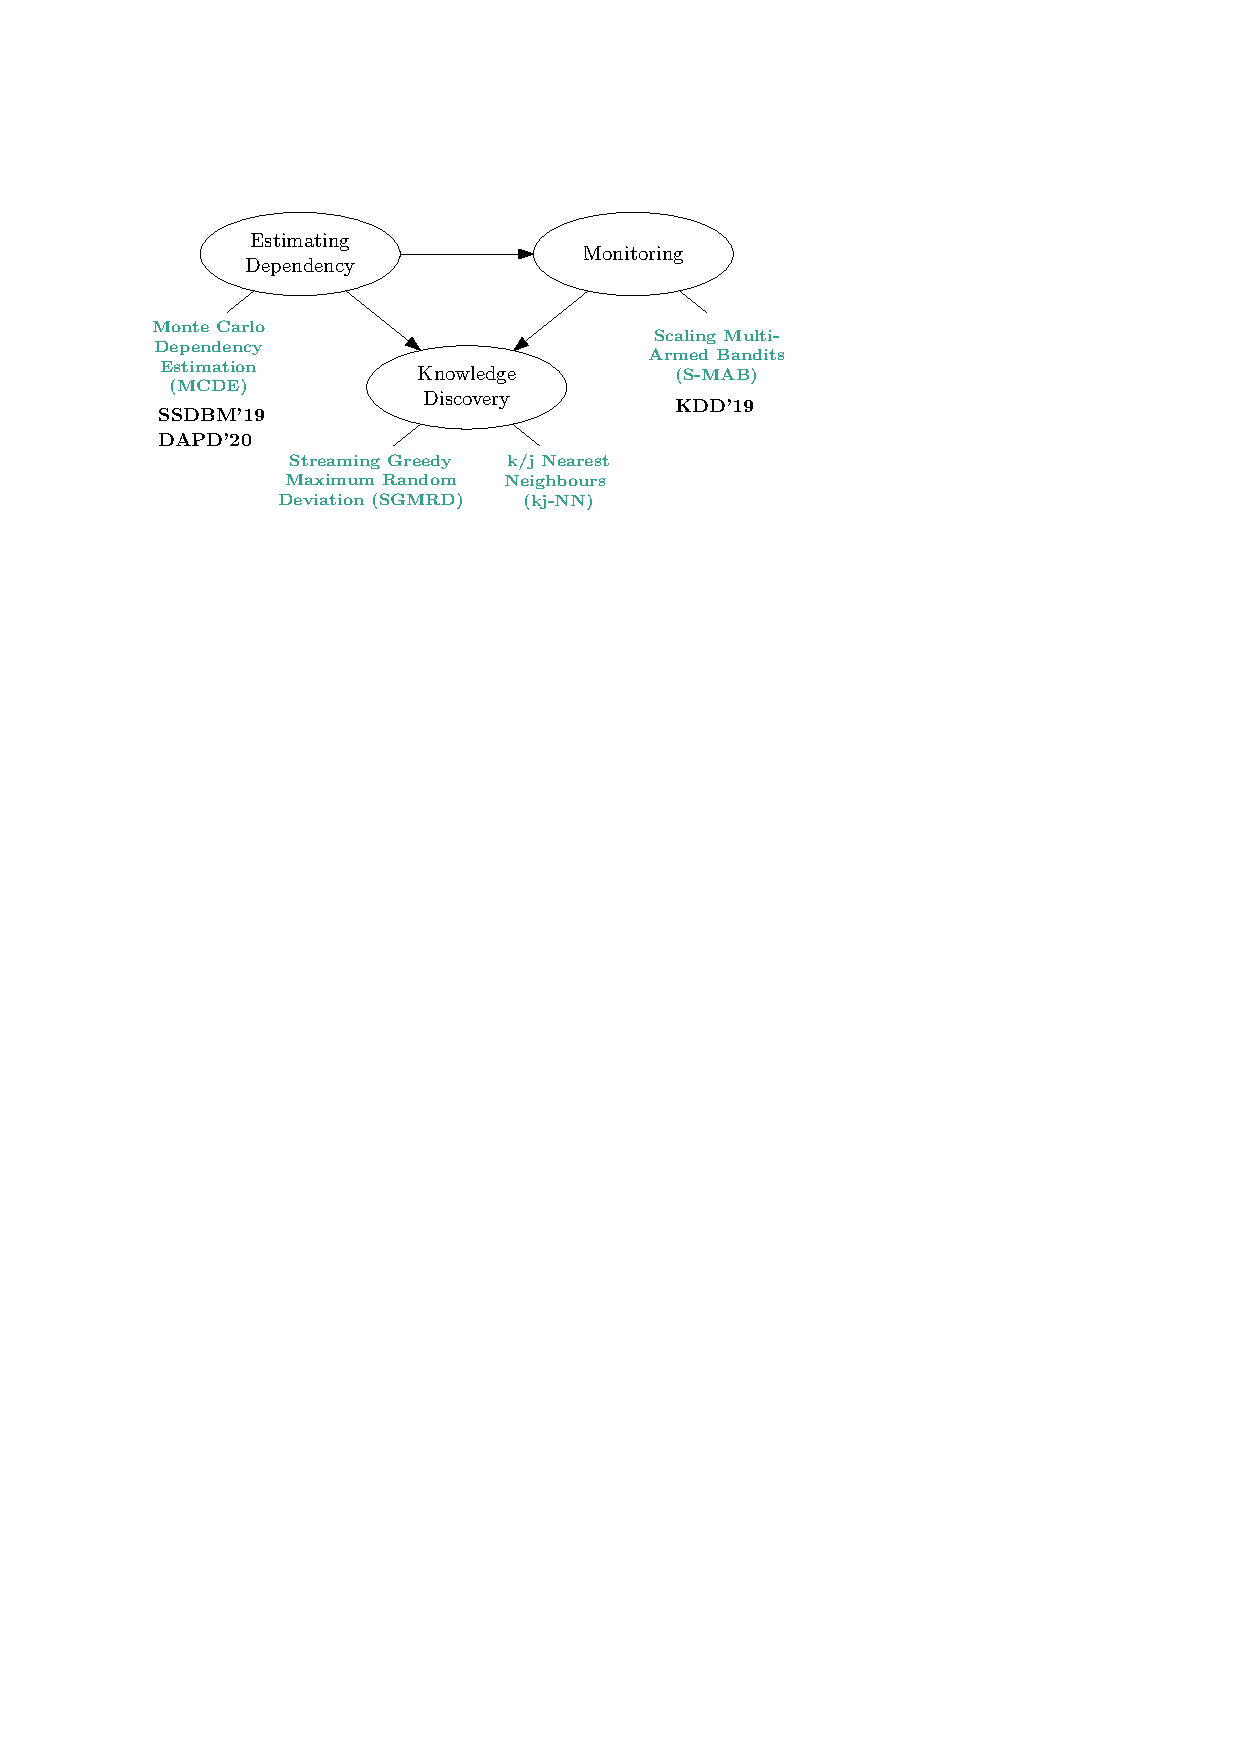
\includegraphics[width=1.0 \linewidth]{figures/outline_c_8-compressed.pdf}
	\end{overprint}
\end{figure}
\vspace{-0.7cm}

% In the first part, we address the question about estimating dependency. We propose Monte Carlo Dependency Estimation, a framework to estimate dependency in high-dimensional data streams. Then, we formulate the problem of monitoring statistics as a Multi-Armed Bandit problem. We extend the existing models by proposing the so-called "Scaling Multi-Armed Bandits". Finally, we exploit the synergies between those two contributions and combine the ideas behind MCDE and S-MAB to facilitate subspace search in data streams. We show that our idea, Streaming Greedy Maximum Random Deviation, leads to outstanding results w.r.t. Knowledge Discovery tasks, such as outlier detection. Then, we propose the kj- Nearest Neighbours, a new method to detect outlying documents in large text corpora.

% We published our findings about MCDE in the proceedings of the SSDBM conference last year, where we obtained the best paper award. We recently published a follow-up study in the Distributed and Parallel Databases journal. On the other side, we published the Scaling Multi-Armed Bandits in the proceedings of the KDD conference last year. The other two significant contributions are currently under review. For this reason, and because of time restrictions, I will focus during the rest of this presentation on those first two items: Monte Carlo Dependency Estimation and the Scaling Multi-Armed Bandits. 
\end{frame}

\section{Estimating Dependency}

\begin{frame}{Monte Carlo Dependency Estimation}
%Basic idea:

For any given subspace $S = \{X_1, \dots, X_d\}$:

\begin{itemize}
	\item We see each dimension $X_i \in S$ as a random variable:  
\end{itemize}
\pause

\begin{overprint}
	\onslide<1-2> 
	\begin{center}
		$\overbrace{p(S) = \prod_{X_{i} \in S} p_{X_i}(S)}^{\mathclap{independence}} 
		\quad \Rightarrow \quad \forall X_i \in S,   \textcolor{specialorange}{\overbrace{p_{X_i}(S)}^{\mathclap{marginal}}} = \textcolor{specialblue}{{\underbrace{p(S|\overline{X_i})}_{\mathclap{conditional}}}}$
	\end{center}
	\onslide<3-> 
	\begin{center}
	$ \underbracket{\overbrace{p(S) = \prod_{X_{i} \in S} p_{X_i}(S)}^{\mathclap{independence}}}_{\textcolor{uiucred}{\mathlarger{A}}} \quad \Rightarrow \quad \underbracket{\forall X_i \in S,   \textcolor{specialorange}{\overbrace{p_{X_i}(S)}^{\mathclap{marginal}}} = \textcolor{specialblue}{{\underbrace{p(S|\overline{X_i})}_{\mathclap{conditional}}}}}_{\textcolor{uiucred}{\mathlarger{B}}}
	$
	\end{center}
\end{overprint}
\pause
\pause
\begin{itemize}
	\item Then $\textcolor{uiucred}{\neg B} \Rightarrow \textcolor{uiucred}{\neg A}$ (non-independence)
\pause
\begin{itemize}
	\item Our idea: quantify $\textcolor{uiucred}{\neg B}$ as $discrepancy(\textcolor{specialorange}{p_{X_i}(S)}, \textcolor{specialblue}{{p(S|\overline{X_i})}}), \forall X_{i} \in S$
\end{itemize}
\pause
\begin{itemize}
\item We propose a Monte Carlo method to approximate the $discrepancy$
\end{itemize}
\end{itemize}
\end{frame}

\begin{frame}{Monte Carlo Dependency Estimation}
\vspace{-1cm}
\begin{columns}
	\begin{column}{0.6\textwidth}
		\begin{figure}
			\centering
			\begin{overprint}
				\onslide<1> 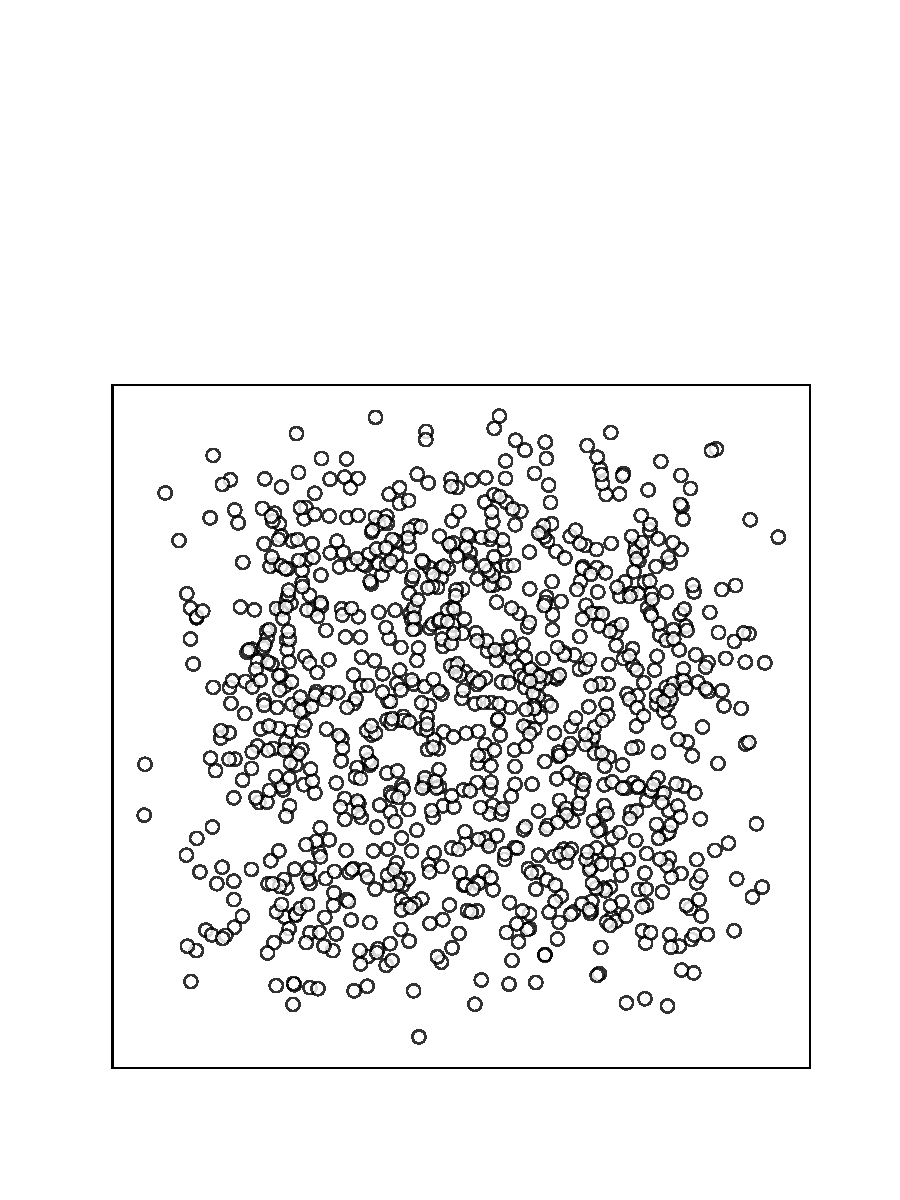
\includegraphics[trim=1cm 1cm 1cm 1cm, width=0.49\linewidth]{figures/independent_2D_0_nomarginal-compressed.pdf}
				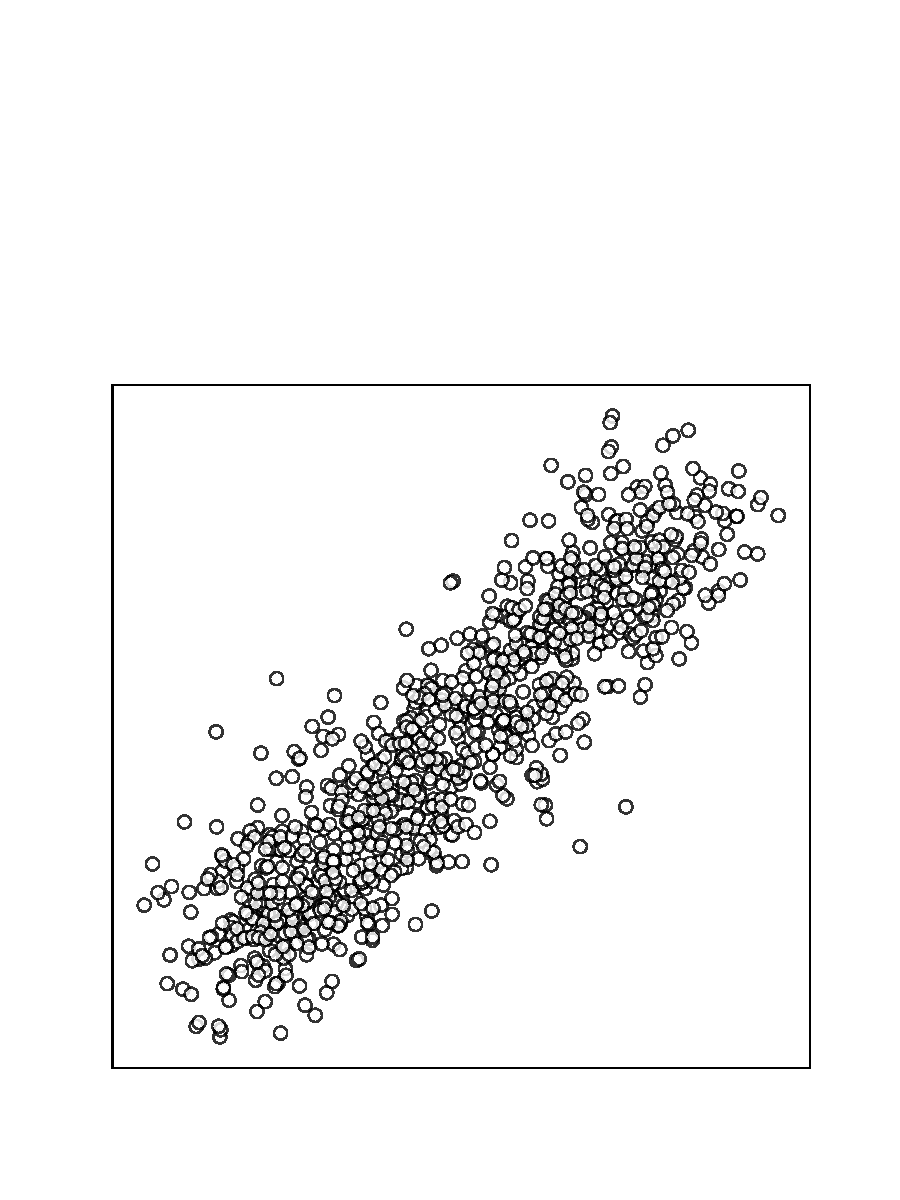
\includegraphics[trim=1cm 1cm 1cm 1cm, width=0.49\linewidth]{figures/linear_2D_0_nomarginal-compressed.pdf}
				\onslide<2> 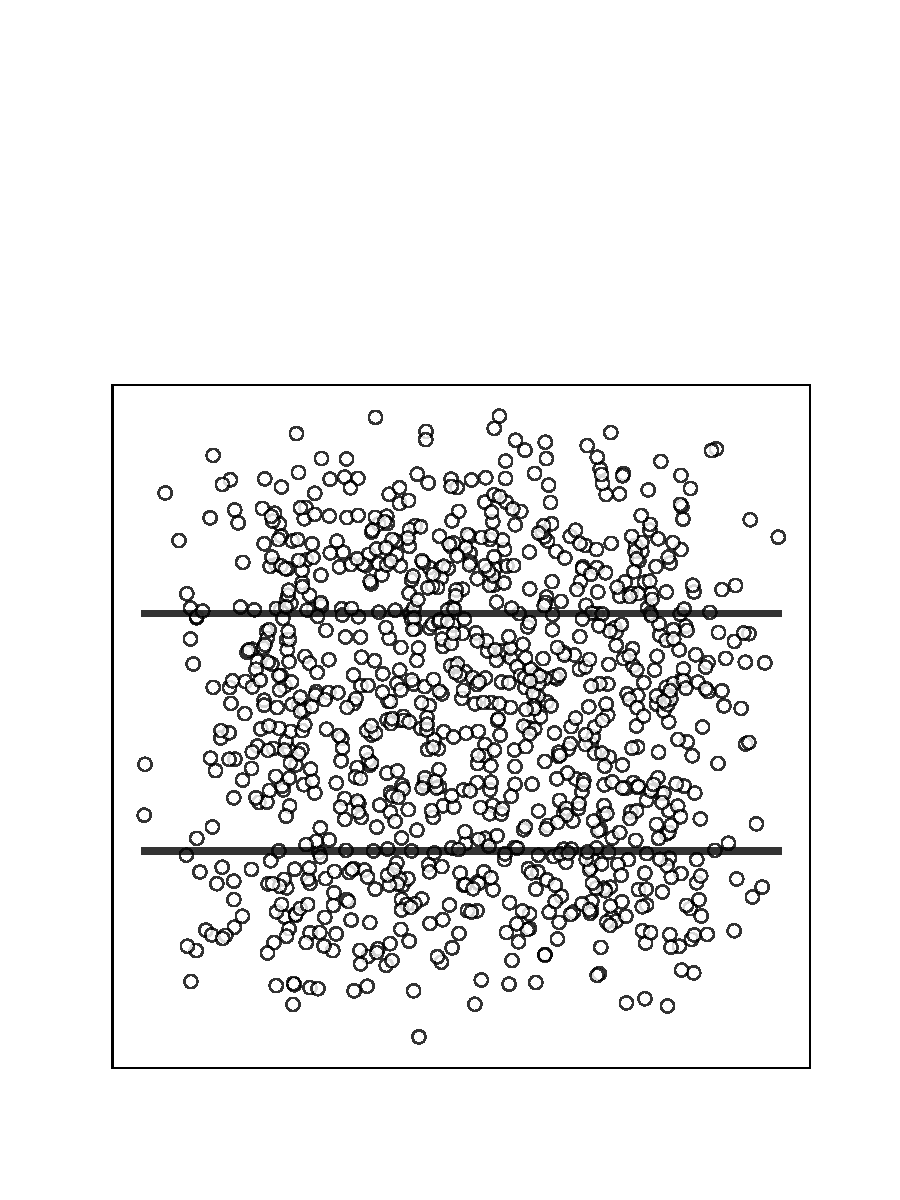
\includegraphics[trim=1cm 1cm 1cm 1cm, width=0.49\linewidth]{figures/independent_2D_1_nomarginal-compressed.pdf}
				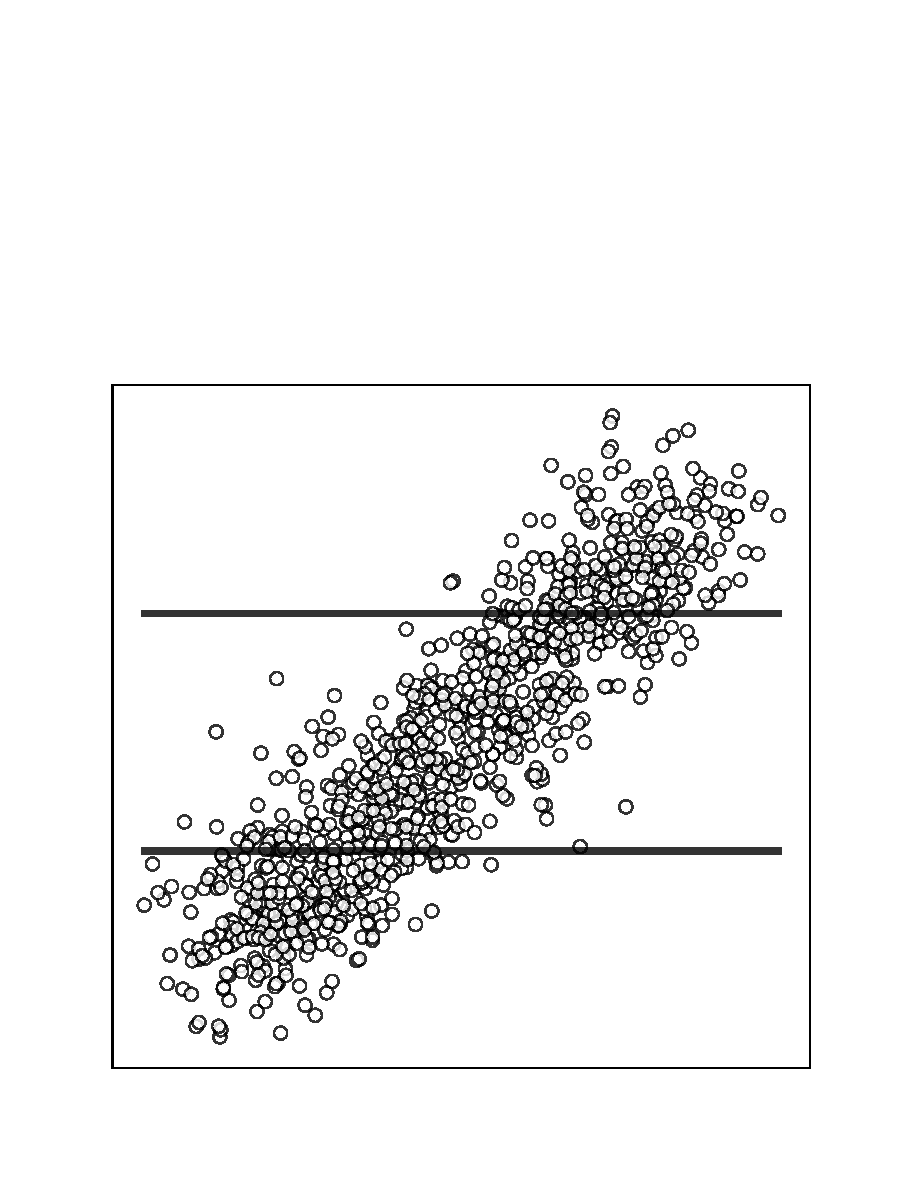
\includegraphics[trim=1cm 1cm 1cm 1cm, width=0.49\linewidth]{figures/linear_2D_1_nomarginal-compressed.pdf}
				\onslide<3> 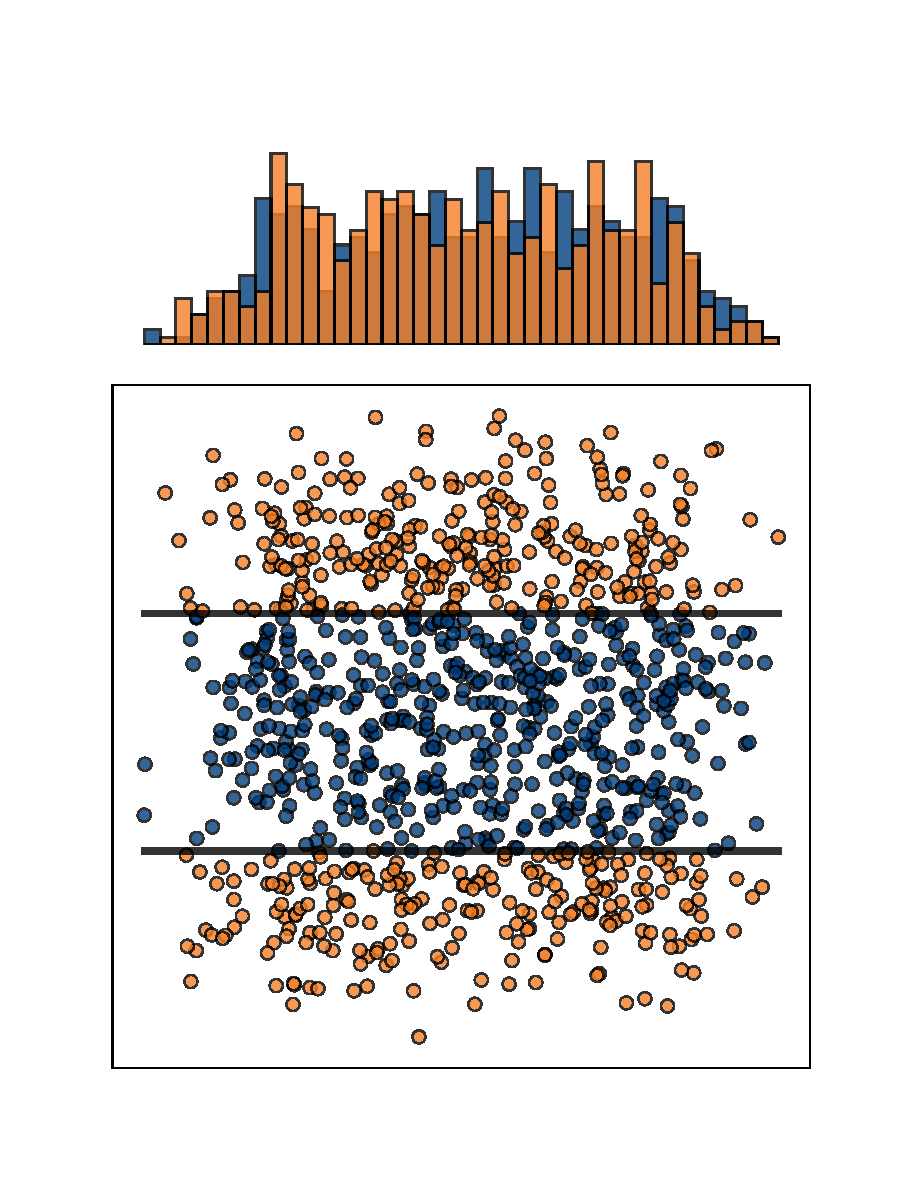
\includegraphics[trim=1cm 1cm 1cm 1cm, width=0.49\linewidth]{figures/independent_2D_2_nomarginal-compressed.pdf}
				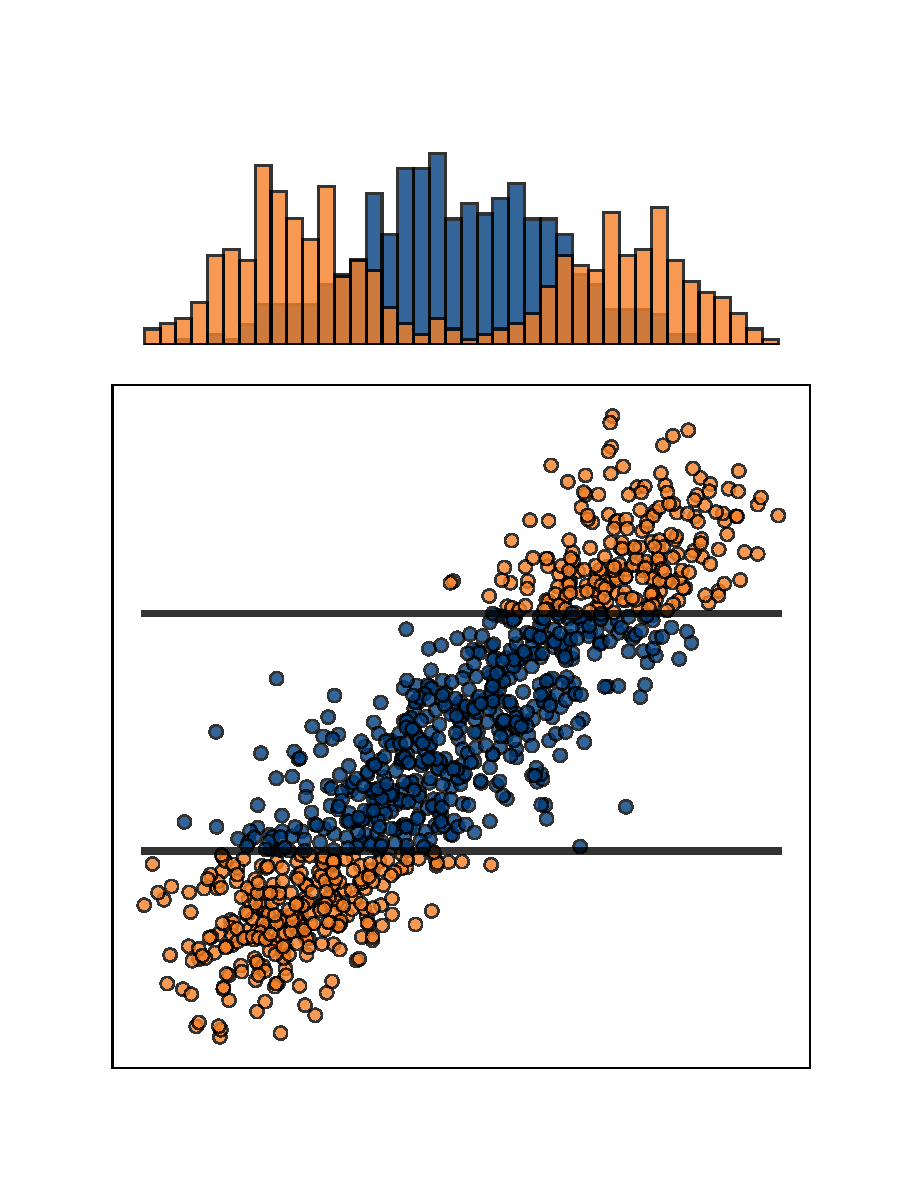
\includegraphics[trim=1cm 1cm 1cm 1cm, width=0.49\linewidth]{figures/linear_2D_2_nomarginal-compressed.pdf}
				\onslide<4> 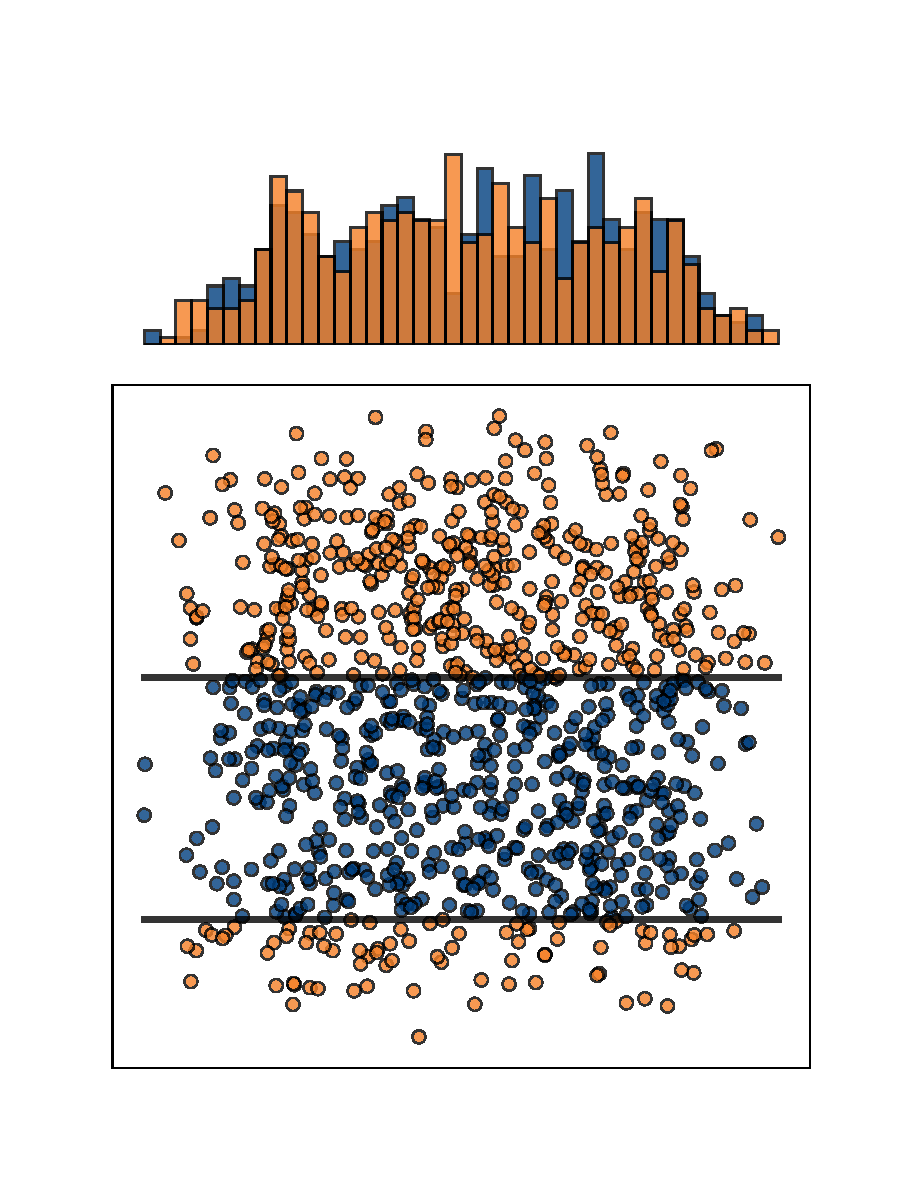
\includegraphics[trim=1cm 1cm 1cm 1cm, width=0.49\linewidth]{figures/independent_2D_3_nomarginal-compressed.pdf}
				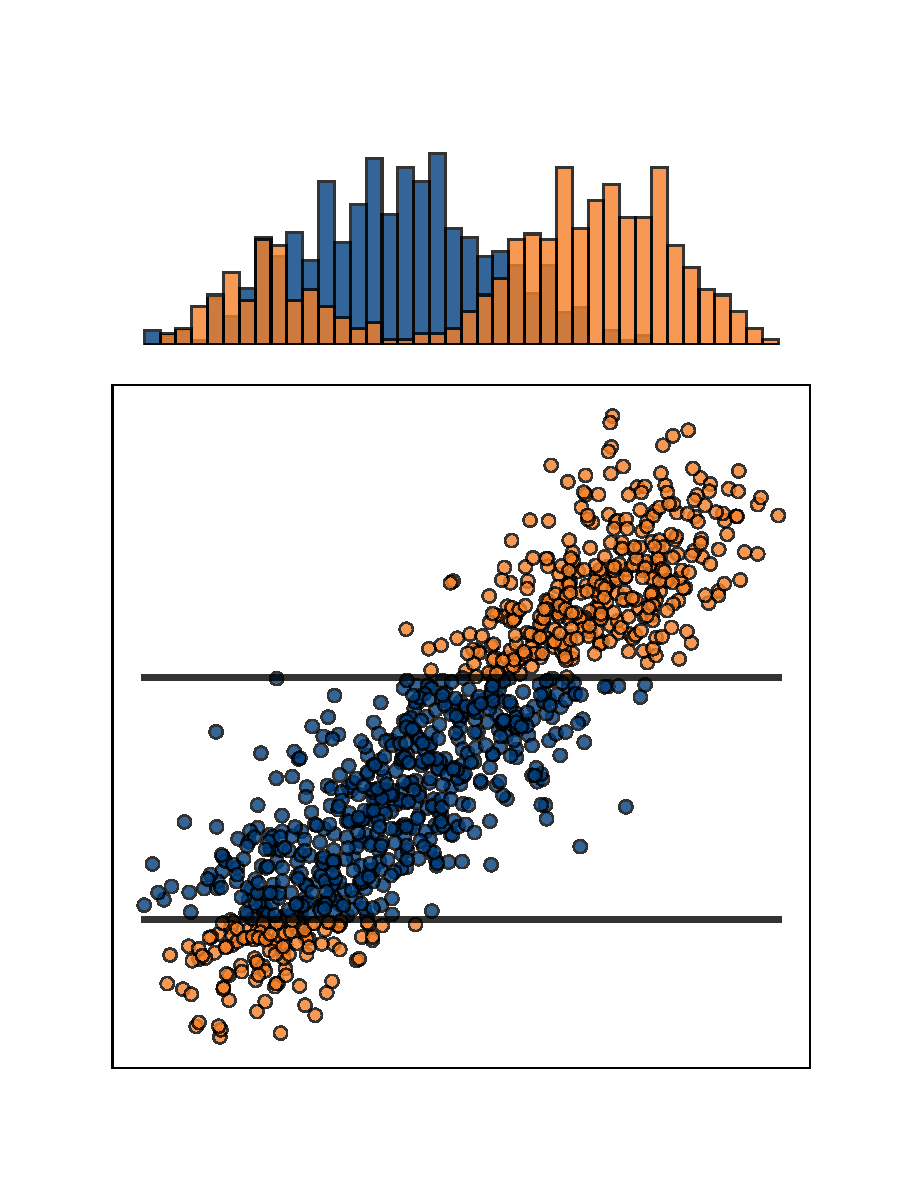
\includegraphics[trim=1cm 1cm 1cm 1cm, width=0.49\linewidth]{figures/linear_2D_3_nomarginal-compressed.pdf}
				\onslide<5-> 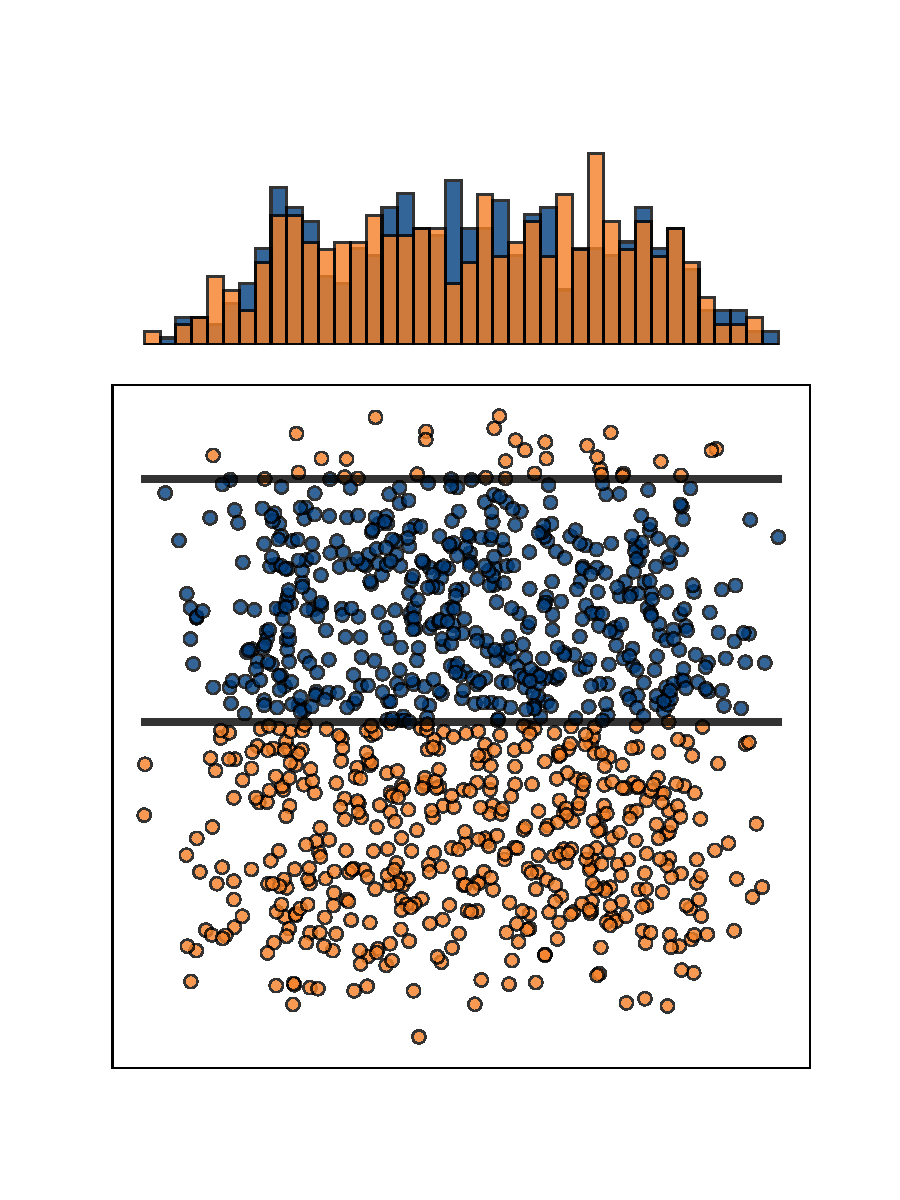
\includegraphics[trim=1cm 1cm 1cm 1cm, width=0.49\linewidth]{figures/independent_2D_4_nomarginal-compressed.pdf}
				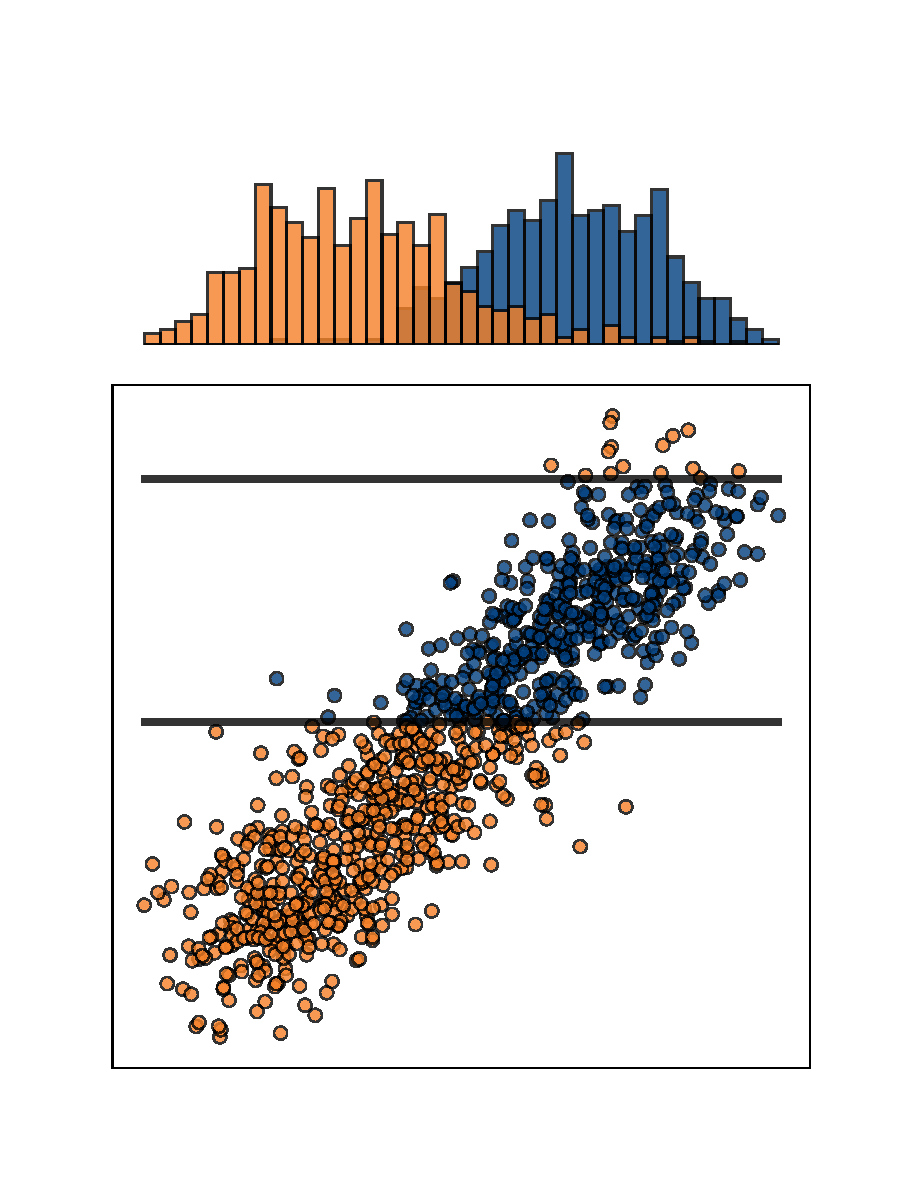
\includegraphics[trim=1cm 1cm 1cm 1cm, width=0.49\linewidth]{figures/linear_2D_4_nomarginal-compressed.pdf}
			\end{overprint}
		\end{figure}
	\end{column}
	\pause
	\begin{column}{0.42\textwidth} 
		\begin{itemize}
			\item Take a random slice
			\pause
			\item Test $\mathcal{T}(\textcolor{specialorange}{\hat{p}_{X_i}(S)},\textcolor{specialblue}{\hat{p}(S|\overline{X_i})})$
			\pause
			\item Repeat $M$ times
			\pause
			\item Average: 
		\end{itemize}
		\pause
		\begin{align*}
		\mathcal{C} = \frac{1}{M} \sum^{M}_{m=1} ( 1- p\text{-}value) 
		\end{align*}
	\end{column}
\end{columns}
\pause
Properties: 
\begin{itemize}
	\item Independence $\Rightarrow \mathbb{E}[\mathcal{C}] = 0.5$, otherwise greater
	\item $\mathcal{C} \in [0,1]$
\end{itemize}
\pause
Theorem (derived from \cite{doi:10.1080/01621459.1963.10500830}): $\Pr\left(| \mathcal{C} - \mathbb{E}[\mathcal{C}] | \geq \varepsilon \right) \leq 2e^{-2M \varepsilon^2}$

~\\

\end{frame}

\begin{frame}{MCDE: A General Estimation Framework}
\begin{center}
\begin{columns}
	\begin{column}{0.38\textwidth}
		\vspace{-0.25cm}
		{\small
		\begin{itemize}
			\item Non-linear dependencies
		\end{itemize}
		}
		\vspace{-0.25cm}
	\begin{center}
		\begin{figure}
			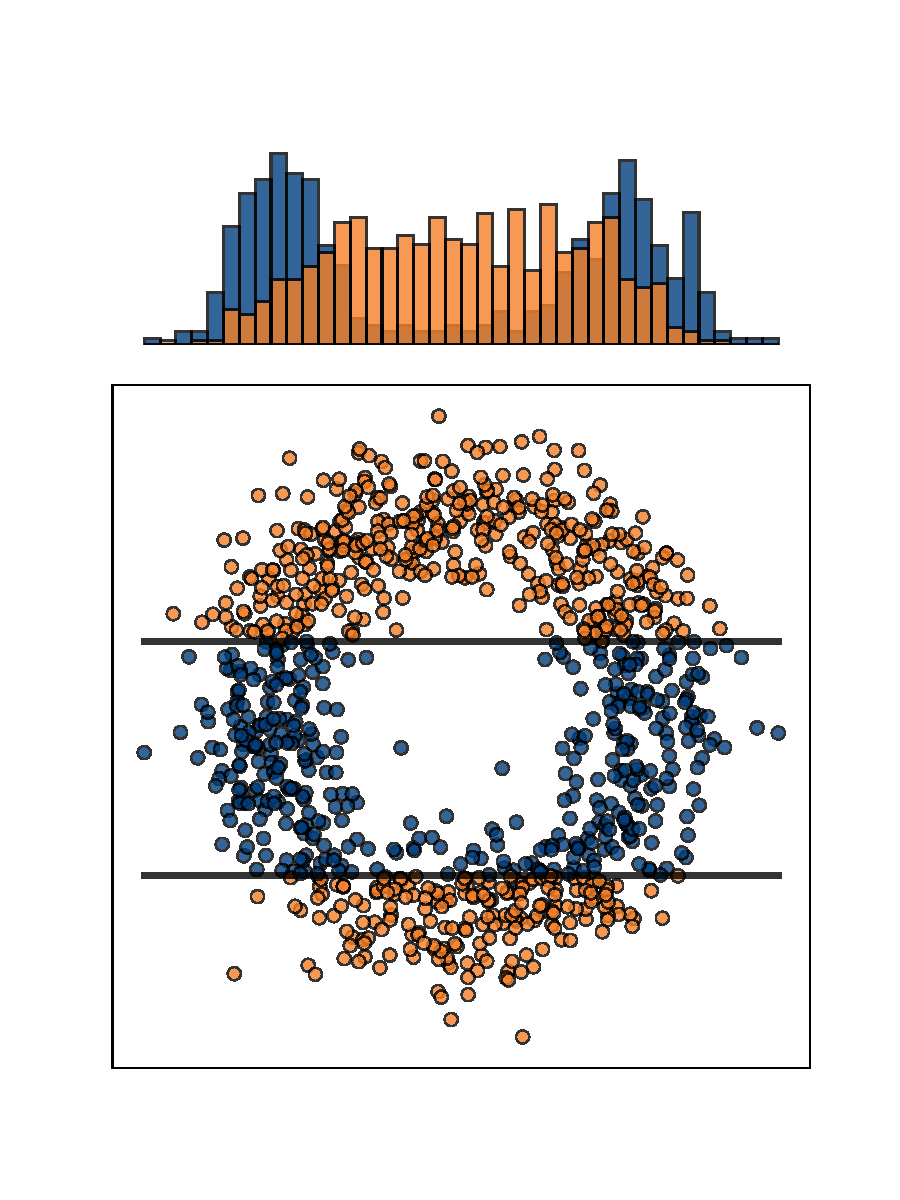
\includegraphics[trim=1cm 1cm 1cm 1cm, width=0.45\linewidth]{figures/circle_2D_nomarginal-compressed.pdf}
			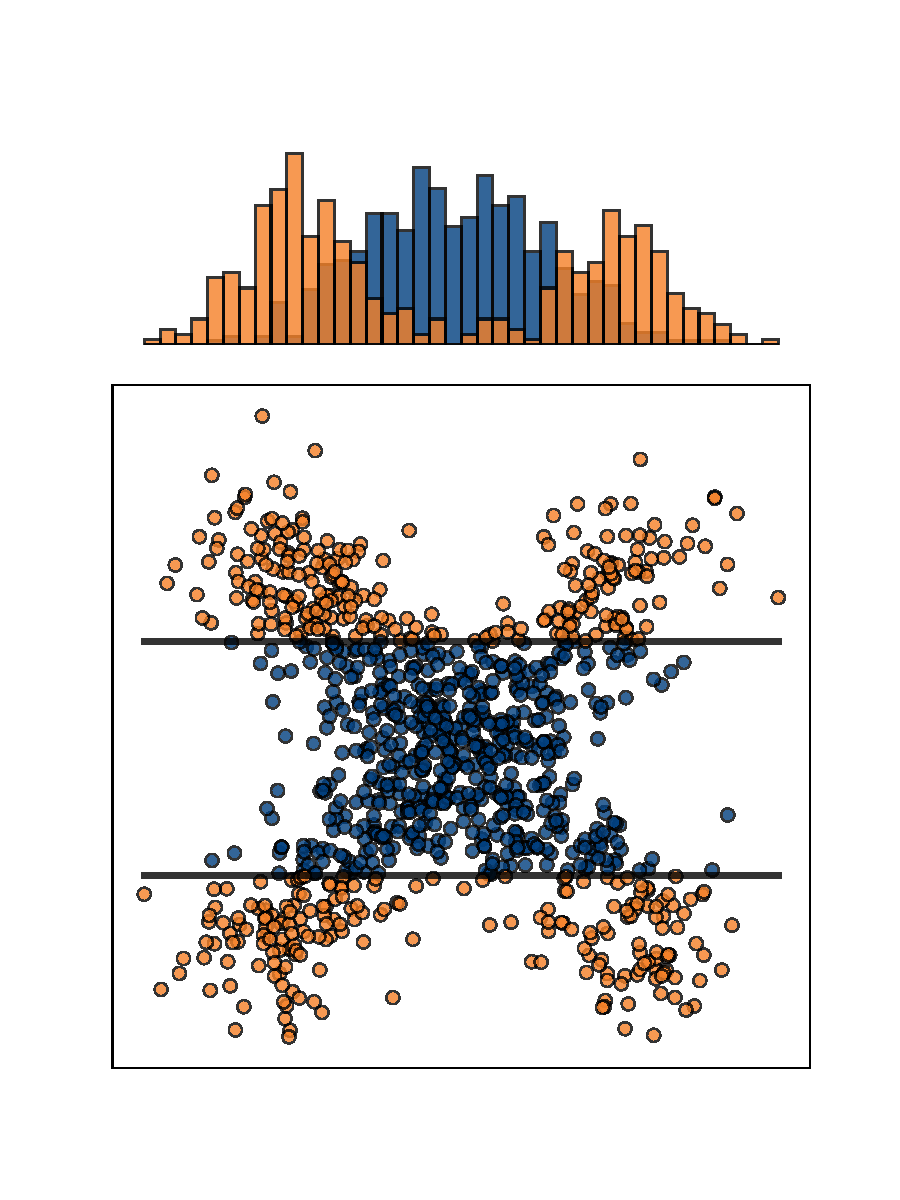
\includegraphics[trim=1cm 1cm 1cm 1cm, width=0.45\linewidth]{figures/cross_2D_nomarginal-compressed.pdf}
			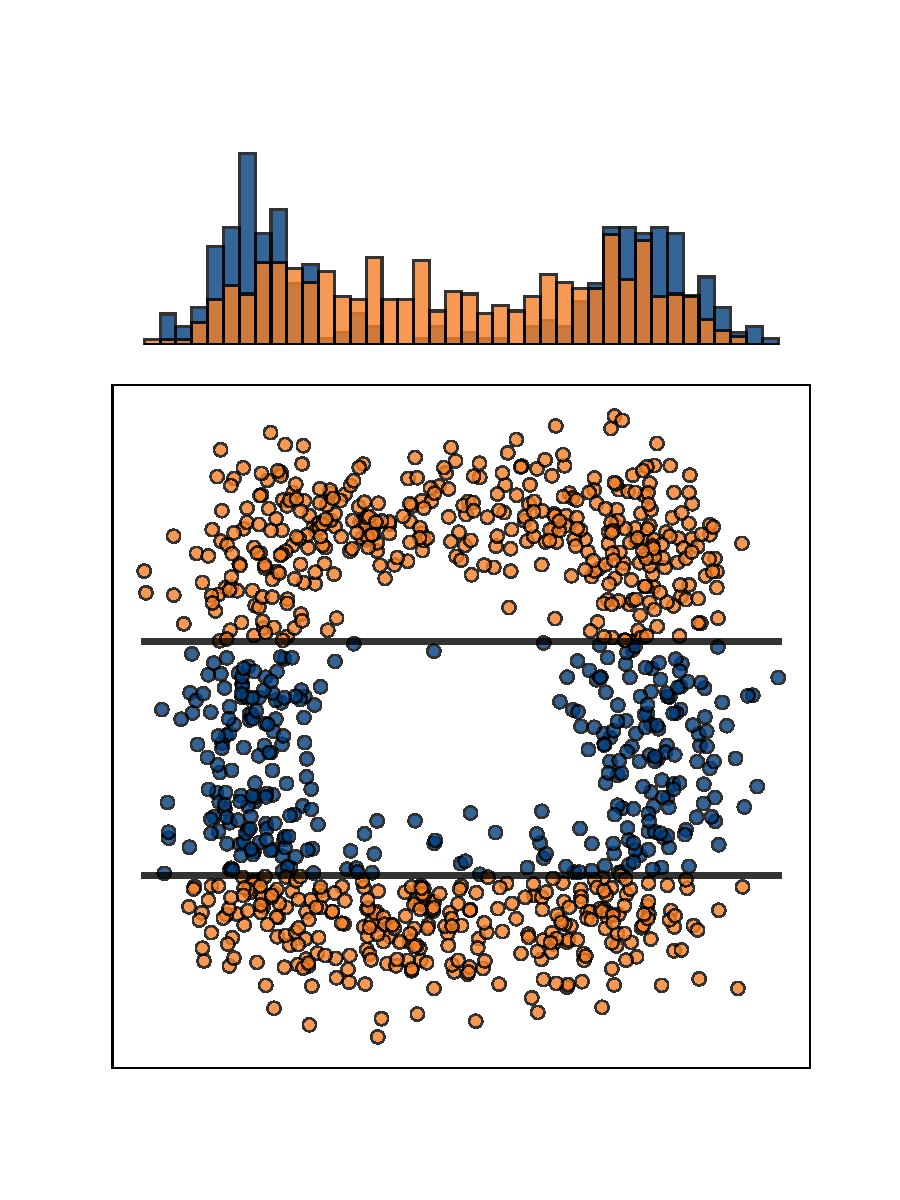
\includegraphics[trim=1cm 1cm 1cm 1cm, width=0.45\linewidth]{figures/square_2D_nomarginal-compressed.pdf}
			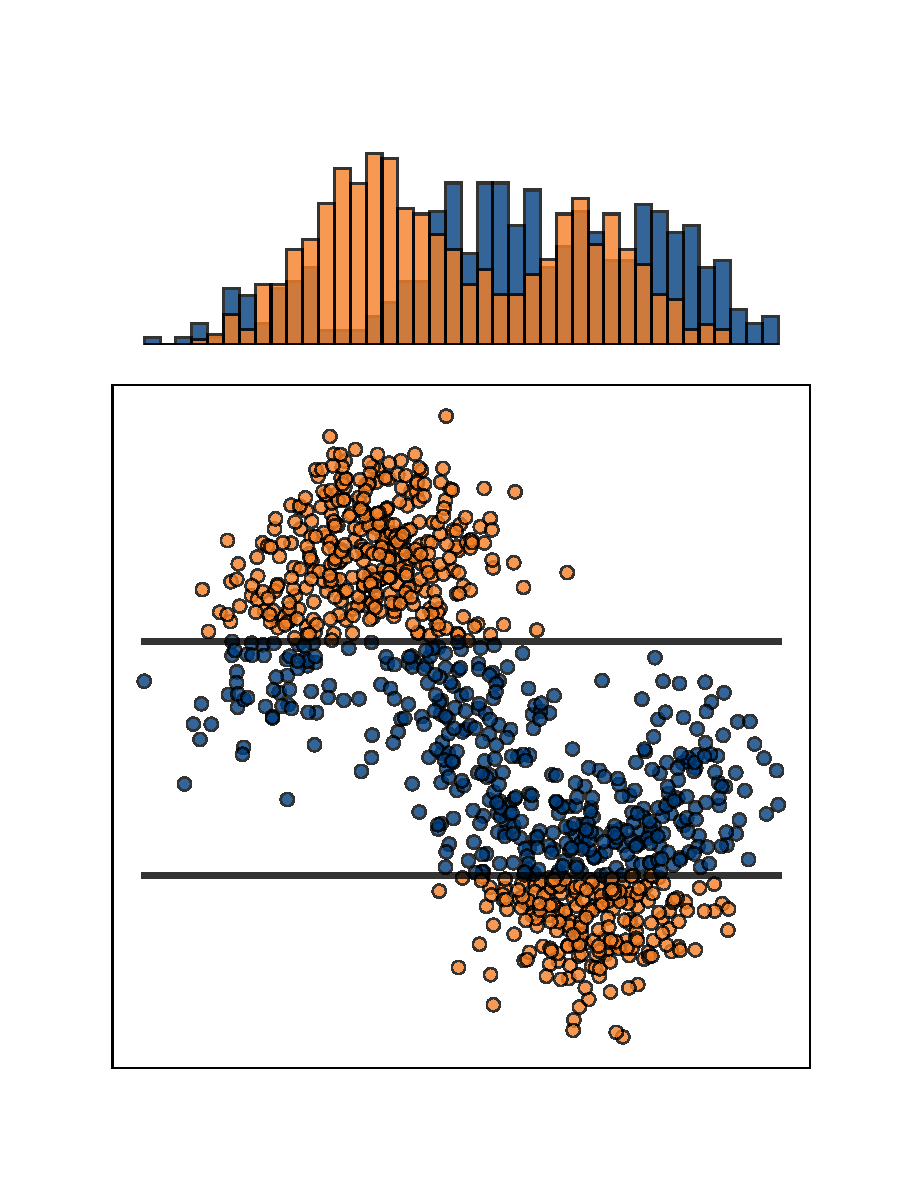
\includegraphics[trim=1cm 1cm 1cm 1cm, width=0.45\linewidth]{figures/sine_2D_nomarginal-compressed.pdf}
		\end{figure}
	\end{center}
		
	\end{column}
	\vrule{} 
	\begin{column}{0.58\textwidth}
		{\small
			\begin{itemize}
				\item Multivariate data
			\end{itemize}
		}
		\vspace{-0.25cm}
		\begin{figure}
			\hfill
			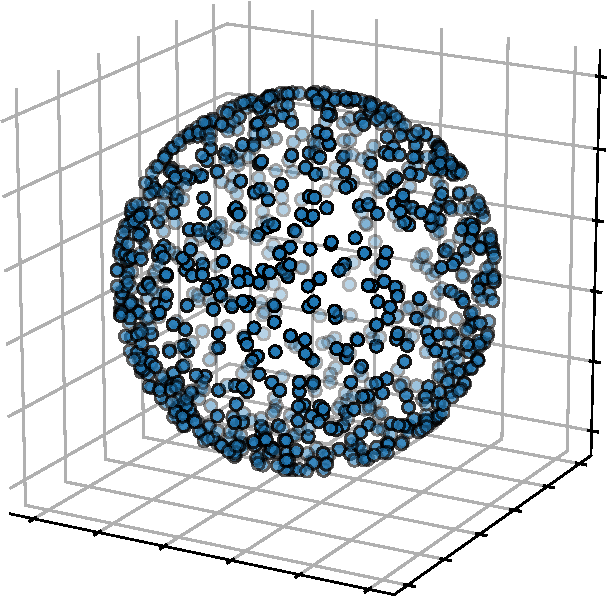
\includegraphics[width=0.22\linewidth]{figures/Sphere-3-00-crop-compressed.pdf}
			\hfill
			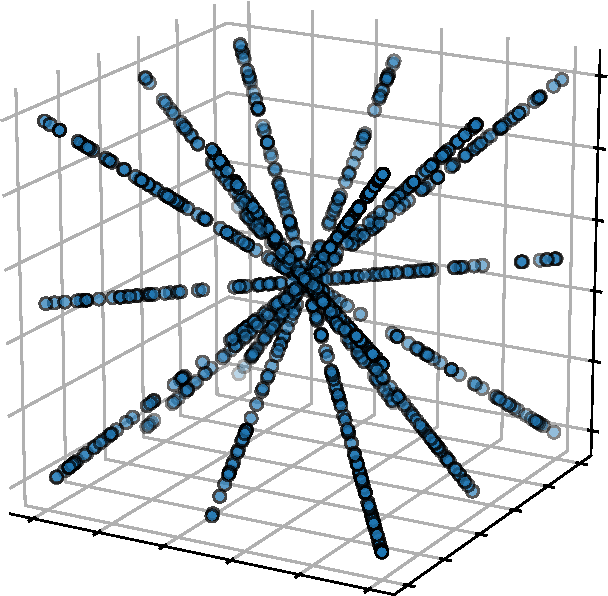
\includegraphics[width=0.22\linewidth]{figures/Star-3-00-crop-compressed.pdf}
			\hfill
			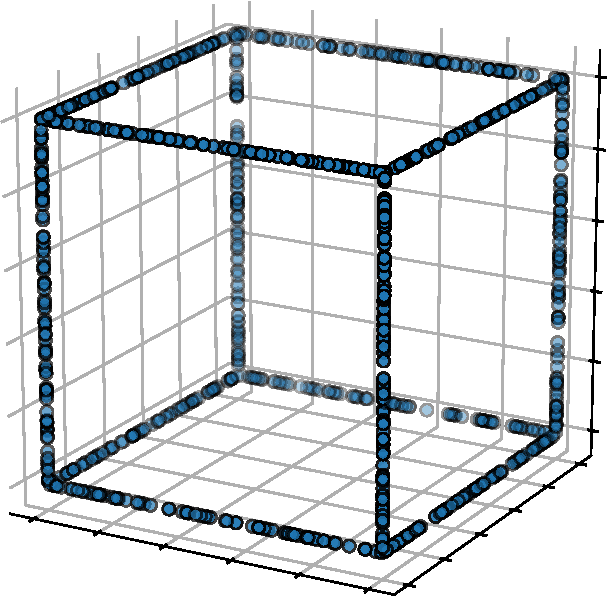
\includegraphics[width=0.22\linewidth]{figures/Hollowcube-3-00-crop-compressed.pdf}
			\hfill
			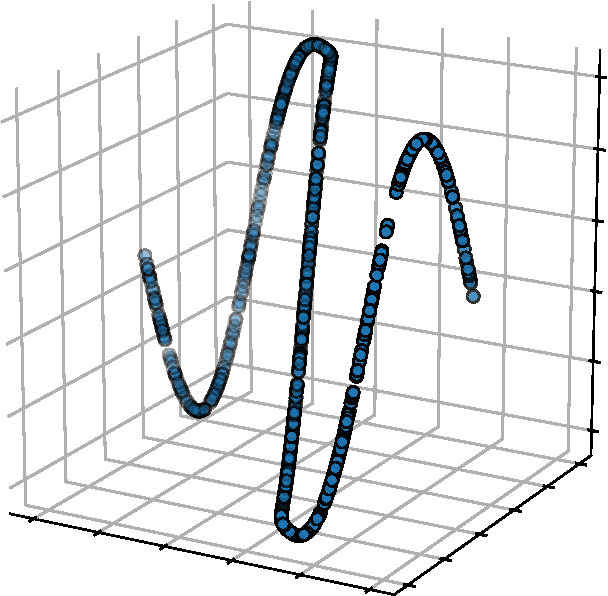
\includegraphics[width=0.22\linewidth]{figures/Sine_1-3-00-crop-compressed.pdf}
			\hfill
		\end{figure}
		\vspace{-0.75cm}
		\begin{center}
			\rule{0.9\linewidth}{ .1mm}
		\end{center}
	    \vspace{-0.5cm}
	    {\small
	    	\begin{itemize}
	    		\item Heterogeneous data
	    	\end{itemize}
	    }
    	\vspace{-0.4cm}
	    \begin{figure}
			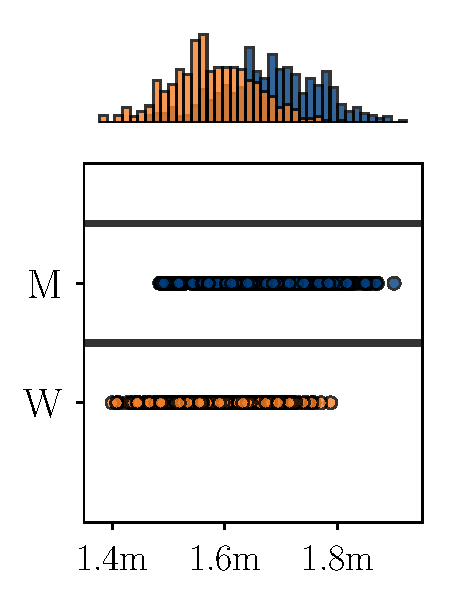
\includegraphics[ width=0.30\linewidth]{figures/mixed_1_2D_hetero2_defense-compressed.pdf}
			\hfill
			\includegraphics[ width=0.30\linewidth]{figures/mixed_0_2D_hetero1_defense-compressed.pdf}
			\hfill
			\includegraphics[ width=0.30\linewidth]{figures/mixed_0_2D_homo2_defense-compressed.pdf}
		\end{figure}
	\end{column}
\end{columns}
\end{center}
\end{frame}

\begin{frame}{Evaluating MCDE}

We systematically assess MCDE against 12 requirements.  
\vspace{-0.25cm}
\begin{figure}
	\begin{overprint}
		\onslide<1> \includegraphics[trim=0.5cm 0 0.5cm 0, width=1.0\linewidth]{figures/table_requirements_1-small.jpg}
		%\onslide<2> \includegraphics[trim=0.5cm 0 0.5cm 0, width=1.0\linewidth]{figures/table_requirements_2-small.jpg}
		\onslide<2> \includegraphics[trim=0.5cm 0 0.5cm 0, width=1.0\linewidth]{figures/table_requirements_3-small.jpg}
		\onslide<3-> \includegraphics[trim=0.5cm 0 0.5cm 0, width=1.0\linewidth]{figures/table_requirements_4-small.jpg}
	\end{overprint}
\end{figure}
\vspace{-0.75cm}
{\footnotesize $^*$ \cite{SCHMID2007407}, $^{**}$ \cite{DBLP:journals/ibmrd/Watanabe60}, $^{***}$ \cite{DBLP:journals/tit/McGill54}, $^{\dagger}$ \cite{DBLP:conf/sdm/BohmKMNV13}, $^{\ddagger}$  \cite{DBLP:conf/icml/NguyenMVEB14}, $^{\ddagger\ddagger}$ \cite{DBLP:conf/sdm/NguyenMV16}, $^\$ \cite{DBLP:conf/icde/KellerMB12}$}
\pause
\pause
\begin{itemize}
	\item MCDE outperforms the competitors w.r.t. those requirements
\end{itemize}
\end{frame}

\begin{frame}{Deploying MCDE @ Bioliq}

\begin{itemize}
	\item We estimated MCDE during 4 days at Bioliq between 20 sensors
	\pause
	\begin{itemize}
		\item We presented $20$ patterns to the plant operators 
		\pause
		\item They found that $6$ of them were very interesting (here is one of them)
	\end{itemize}
\end{itemize}

\begin{figure}
	\centering
	\begin{overprint}
		\onslide<3> \includegraphics[width=0.95\linewidth]{figures/Dep_example_thesis_2_0-compressed.pdf}
		\onslide<4> \includegraphics[width=0.95\linewidth]{figures/Dep_example_thesis_2_1-compressed.pdf}
		\onslide<5> \includegraphics[width=0.95\linewidth]{figures/Dep_example_thesis_2_2-compressed.pdf}
		\onslide<6> \includegraphics[width=0.95\linewidth]{figures/Dep_example_thesis_2_3-compressed.pdf}
		\onslide<7-> \includegraphics[width=0.95\linewidth]{figures/Dep_example_thesis_2_4-compressed.pdf}
		%\includegraphics[width=0.8 \linewidt]{figures/bioliq_prep_s-crop-compressed.pdf}
	\end{overprint}
	\begin{overprint}
		\onslide<4> \includegraphics[ width=0.95\linewidth]{figures/Dep_example_details_thesis-compressed_1-compressed.pdf}
		\onslide<5> \includegraphics[ width=0.95\linewidth]{figures/Dep_example_details_thesis-compressed_2-compressed.pdf}
		\onslide<6> \includegraphics[ width=0.95\linewidth]{figures/Dep_example_details_thesis-compressed_3-compressed.pdf}
		\onslide<7> \includegraphics[ width=0.95\linewidth]{figures/Dep_example_details_thesis-compressed.pdf}
		%\includegraphics[width=0.8 \linewidt]{figures/bioliq_prep_s-crop-compressed.pdf}
	\end{overprint}
	%\caption{Example of an interesting dependency pattern in the pyrolysis data}
	\label{fig:real-world-pattern}
\end{figure}

\end{frame}

\section{Monitoring}

\begin{frame}{From Estimating to Monitoring}

Now, we are able to estimate dependency in HD-DS. 

~\\
\begin{overprint}
	\onslide<1> \includegraphics[width=7cm,scale=0.5]{figures/correlation_matrix_bis_1.pdf}
	\onslide<2> \includegraphics[width=7cm,scale=0.5]{figures/correlation_matrix_bis_2.pdf}
	\onslide<3> \includegraphics[width=7cm,scale=0.5]{figures/correlation_matrix_bis_3.pdf}
	\onslide<4-> \includegraphics[width=7cm,scale=0.5]{figures/correlation_matrix_bis_4.pdf}
\end{overprint}

\pause
\pause
\begin{itemize}
	\item However, there are too many pairs/subspaces 
	\pause
	\item Only a few pairs/subspaces are actually interesting
	\begin{itemize}
		\item Others have low correlation, or never change
	\end{itemize}  
	\pause
	\item We can reduce the cost of monitoring if we find them
	\begin{itemize}
		\item Which? How many? 
	\end{itemize} 
\end{itemize}

\end{frame}

\begin{frame}{Monitoring as Multi-Armed Bandit (MAB)}

%Basic idea: Model monitoring as a Multi-Armed Bandit (MAB) problem
\begin{figure}
	\centering
	\begin{overprint}
		\onslide<1>
	\includegraphics[width=1\linewidth]{figures/bandit_1tok_big_alice_3-compressed.pdf}
		\onslide<2>
	\includegraphics[width=1\linewidth]{figures/bandit_1tok_big_alice_2-compressed.pdf}
		\onslide<3>
	\includegraphics[width=1\linewidth]{figures/bandit_1tok_big_alice_1-compressed.pdf}
		\onslide<4->
	\includegraphics[width=1\linewidth]{figures/bandit_1tok_big_alice_0-compressed.pdf}
	\end{overprint}
\end{figure}

\pause
\pause 
\pause
\pause

\begin{columns}
	\begin{column}{0.50\textwidth}
		{\small
			To maximise our gain, we need to find: 
			\begin{itemize}
				\item Which arms are the best? 
				\item How many arms to play? 
				\item When to adapt?  
			\end{itemize}
		}
	\end{column}
	\hspace{-0.25cm}
	\vrule{}
	\hspace{0.25cm}
	\begin{column}{0.39\textwidth} 
		\begin{overprint}[0.7\textwidth]
			\onslide<6>
			\begin{tikzpicture}[remember picture,overlay]
			\node[anchor=south east,inner sep=0pt] at ($(current page.south east)+(-1.3cm,1.5cm)$) {
				\includegraphics[angle=0, width=3.5cm]{figures/correlation_matrix_bis_5-compressed.pdf}
			};
			\end{tikzpicture}
		\end{overprint}
	\end{column}
\end{columns}

~\\

%\pause
%$\rightarrow$ Existing bandit models do not capture this setting. 

~\\

%KDD promotional video (3 minutes) (\href{https://www.dropbox.com/s/92trha3049f9ae9/S-MAB_FOUCHE_KDD19_VIDEO.mp4}{\textcolor{blue}{\underline{dropbox}}}) 
\end{frame}

\begin{frame}{Bandit Models}
\begin{overprint}
	\onslide<2>
	\begin{tikzpicture}[remember picture,overlay]
	\node[anchor=south east,inner sep=0pt] at ($(current page.south east)+(-1.0cm,1.5cm)$) {
		\includegraphics[angle=0, width=4cm]{figures/bandit_K_multiple_1-compressed.pdf}
	};
	\end{tikzpicture}
	\onslide<3>
	\begin{tikzpicture}[remember picture,overlay]
	\node[anchor=south east,inner sep=0pt] at ($(current page.south east)+(-1.0cm,1.5cm)$) {
		\includegraphics[angle=0, width=4cm]{figures/bandit_K_multiple_2-compressed.pdf}
	};
	\end{tikzpicture}
	\onslide<4>
	\begin{tikzpicture}[remember picture,overlay]
	\node[anchor=south east,inner sep=0pt] at ($(current page.south east)+(-1.0cm,1.5cm)$) {
		\includegraphics[angle=0, width=4cm]{figures/bandit_K_multiple_3-compressed.pdf}
	};
	\end{tikzpicture}
	\onslide<5>
	\begin{tikzpicture}[remember picture,overlay]
	\node[anchor=south east,inner sep=0pt] at ($(current page.south east)+(-1.0cm,1.5cm)$) {
		\includegraphics[angle=0, width=4cm]{figures/bandit_K_multiple_4-compressed.pdf}
	};
	\end{tikzpicture}
\end{overprint}
\vspace{-0.5cm}
{\footnotesize
\textbf{Problem:} Existing models do not capture our setting

~\\
\pause

\textbf{The ``Classical'' MAB:}
\begin{itemize}
	\item Only one play per round. \cite{Thompson1933, DBLP:conf/alt/KaufmannKM12}
	\item The environment is static (no change).
\end{itemize}
\pause
\textbf{MAB with Multiple Plays (MP-MAB):} 
\begin{itemize}
	\item $L > 1$ plays per round \cite{DBLP:conf/alt/UchiyaNK10, DBLP:conf/icml/KomiyamaHN15}. 
	\item Assumes a static setting; $L$ is a constant. %anantharam1987asymptotically
	%\item \cite{DBLP:conf/icml/KomiyamaHN15} shows optimal regret of Thompson Sampling \cite{Thompson1933}.% with multiple plays.
\end{itemize}
\pause
\textbf{Non-static MAB:}
\begin{itemize}
	\item Integrate a forgetting mechanism \cite{DBLP:journals/siamcomp/AuerCFS02, DBLP:conf/alt/GarivierM11}.
	\item Usually: sliding window, exponential weighting.
	\item Single-play; Difficult parameter setting. 
\end{itemize} 

~\\
\pause
\textbf{$\rightarrow$ We invent the Scaling Multi-Armed Bandit (S-MAB):}
\begin{itemize}
	\item A MP-MAB with a dynamic number of plays.
	\item Supports the non-static setting.
	%\item The trade-off may change over time
\end{itemize}
}

\end{frame}

\begin{frame}{The Scaling Multi-Armed Bandit (S-MAB)}

\textbf{Idea:} S-MAB solves the following constrained optimisation problem:
\begin{equation}
\underbrace{\underset{I_t \subset [K]}{\max}}_{\mathclap{Set~of~arms}} \overbrace{\sum_{i \in I_t} S_i(t)}^{\mathclap{Sum~of~rewards}} \quad s.t. \quad \underbrace{\eta_t = \frac{\sum_{i \in I_t} \mu_i}{|I_t|}}_{\mathclap{Average~expected~reward}}  > \overbrace{\eta^*}^{\mathclap{Efficiency}} 
\label{eq1}
\end{equation} 

\pause 
If the player always chooses the best arms, then the problem is equivalent to finding an optimal number of plays $L^*$: 
\begin{equation} \label{eq2}
L^* = \underset{{1 \leq L \leq K}}{\max}{L} 
\quad s.t. \quad \underbrace{\frac{\sum_{i=1}^{L} \mu_i}{L}}_{\mathclap{Average~expected~reward\atop~from~the~top\text{-}L~arms}} > \eta^*
\end{equation}
\end{frame}

\begin{frame}{General Scaling Multi-Armed Bandit}

{\small
	Two components for success: $\overbrace{\underline{\text{finding the top-arms}}}^{\text{Existing bandits}}$ + $\overbrace{\underline{\text{finding }L^*}}^{\text{New !}}$
	\pause 
	
	~\\
	
	At each round $t = 1,\dots,T$:
	\begin{itemize}
		\item $1$. The player \underline{chooses} $I_t$ with $|I_t|=L_t$, and observes a reward vector $X_t$
		\item $2$. They \underline{update} their estimation $\hat{\mu}_i$ for $i \in I_t$
		\item $3$. \textbf{\textcolor{kitgreen}{They choose $L_{t+1}$ ($\rightarrow$ Scaling)}}
	\end{itemize}
	
	~\\
	
	\pause
	There exists many approaches for steps $1,2$:
	\begin{itemize}
		
		\item Multiple-Play Thompson Sampling (MP-TS) \citep{Thompson1933, DBLP:conf/alt/KaufmannKM12, DBLP:conf/icml/KomiyamaHN15} 
		\item UCB-type bandits \citep{DBLP:journals/ml/AuerCF02, DBLP:conf/nips/ChenHLLLL16, DBLP:journals/jmlr/GarivierC11} 
		%\item Exp3.M \citep{auer1995gambling, uchiya2010algorithms}
	\end{itemize}
	
	\pause
	For step 3 $\rightarrow$ We introduce a ``scaling policy'' (see next slide)
	%$\rightarrow$ Our approach is independent from the underlying bandit (``base bandit'') 
}

~\\
\end{frame}

\begin{frame}{Scaling Policy: Kullback-Leibler Scaling}
\begin{overprint}
	\onslide<1> \centering \includegraphics[width=0.9\linewidth]{figures/picture_scaling_5-compressed.pdf}
	\onslide<2> \centering \includegraphics[width=0.9\linewidth]{figures/picture_scaling_4-compressed.pdf}
	\onslide<3> \centering \includegraphics[width=0.9\linewidth]{figures/picture_scaling_3-compressed.pdf}
	\onslide<4> \centering \includegraphics[width=0.9\linewidth]{figures/picture_scaling_2-compressed.pdf}
	\onslide<5> \centering \includegraphics[width=0.9\linewidth]{figures/picture_scaling_1-compressed.pdf}
\end{overprint}
\pause
\pause
{	\begin{center}
	$\widehat{B}_t$ is an upper bound based on Kullback-Leibler divergence \citep{DBLP:journals/jmlr/GarivierC11}
	\end{center}
	
}
\end{frame}

\begin{frame}{Evaluating the S-MAB}

We want to minimise two notions of regret: 
\begin{align*}
\underbrace{\text{Reg}(T) = \sum_{t=1}^{T}{\left[\overbrace{\sum_{i \in I^*_t} \mu_i}^{{Best ~arms}} - \overbrace{\sum_{i \in I_t} \mu_i }^{{Played~arms}}\right]}}_{\text{``}standard\text{''}~regret}
&&  
\underbrace{\text{PReg}(T) = \sum_{t=1}^T  \left| L^* - L_t \right|}_{\text{``}pull\text{''}~regret}
\end{align*}

\pause
$\text{Reg}(T)$ is small $\rightarrow$ Top-$L$ arms identification (step $1,2$) 

$\text{PReg}(T)$ is small $\rightarrow$ Scaling converges to $L^*$ (step $3$)
\pause

{\small
$\rightarrow$ We prove that $\text{Reg}(T)$ and $\text{PReg}(T)$ are in $O(\log T)$ with our scaling policy
\pause

~\\

For the non-static setting: 
\begin{itemize}
	\item We combine S-MAB with \\ Adaptative Window (ADWIN) \cite{DBLP:conf/sdm/BifetG07}
	\item Leads to excellent empirical performance
\end{itemize}
}
\begin{overprint}
	\onslide<4>
	\begin{tikzpicture}[remember picture,overlay]
	\node[anchor=south east,inner sep=0pt] at ($(current page.south east)+(-1.0cm,1.2cm)$) {
		 \includegraphics[width=0.4\linewidth]{figures/adwin_1_short-compressed.pdf}
	};
	\end{tikzpicture}
\end{overprint}
~\\

~\\

\end{frame}

\begin{frame}{Deploying S-MAB @ Bioliq}

\begin{itemize}
	\item Bioliq: Monitoring MI between $20$ sensors, 1 week of data
	%\begin{itemize}
	%	\item MI $> 2$ $\rightarrow$ Reward
	%\end{itemize}
\end{itemize}
\begin{figure}
	\includegraphics[width=0.9\textwidth]{figures/Lt_etat_reduced_defense-compressed.pdf}
\end{figure}
\vspace{-0.5cm}
\begin{itemize}
	\item S-MAB-ADWIN can adapt to non-static streams ! 
\end{itemize}
\end{frame}

\section{Knowledge Discovery}

\begin{frame}{Monitoring $\rightarrow$ Knowledge Discovery}
	
\textbf{Subspace Search in Data Streams} 

\begin{itemize}
	\item Find at any time, a set of ``high-quality'' subspaces
	\begin{itemize}
		\item High-quality subspaces reveal patterns: clusters, outliers, \dots
		\pause
		\item Correlation/Dependency is a good proxy for such ``quality'' 
	\end{itemize}
	
\begin{figure}
	\centering
	\begin{overprint}[0.8\linewidth]
	\onslide<3> \includegraphics[width=\linewidth]{figures/subspace_example_1-compressed.pdf}
	\onslide<4-> \includegraphics[width=\linewidth]{figures/subspace_example_2-compressed.pdf}
	\end{overprint}
\end{figure}

\pause
\pause
\pause
\item They are difficult to find, because we consider HD-DS: 
\begin{itemize}
	\item There are so many subspaces
	\item Interesting subspaces may change over time
\end{itemize}
\end{itemize}

\end{frame}

\begin{frame}{Subspace Search in Data Streams}

\textbf{SGMRD: Streaming Greedy Maximum Random Deviation} 
\begin{itemize}
	\item Extend previous static work (GMD \cite{DBLP:journals/ijdsa/TrittenbachB19}) to streams. 
	\item A two-phase process:
\end{itemize}

\begin{figure}
	\begin{overprint}
		\onslide<1>
		\includegraphics[width=0.9\linewidth]{figures/SGMRD_workflow_6-compressed.pdf}
		\onslide<2>
		\includegraphics[width=0.9\linewidth]{figures/SGMRD_workflow_5-compressed.pdf}
		\onslide<3>
		\includegraphics[width=0.9\linewidth]{figures/SGMRD_workflow_4-compressed.pdf}
		\onslide<4>
		\includegraphics[width=0.9\linewidth]{figures/SGMRD_workflow_3-compressed.pdf}
		\onslide<5>
		\includegraphics[width=0.9\linewidth]{figures/SGMRD_workflow_2-compressed.pdf}
		\onslide<6>
		\includegraphics[width=0.9\linewidth]{figures/SGMRD_workflow_1-compressed.pdf}
	\end{overprint}
	\label{fig:SGMRD_workflow}
\end{figure} 
\end{frame}

\begin{frame}{SGMRD improves Outlier Detection}
\begin{itemize}
	\item We use the subspaces to build an ``ensemble'' outlier detector.
	\pause
	\item We find that our method outperform state-of-the-art detectors.
\end{itemize}

\begin{table}[]
	\sisetup{detect-weight,mode=text}
	\renewrobustcmd{\bfseries}{\fontseries{b}\selectfont}
	\renewrobustcmd{\boldmath}{}
	\centering
	\label{result:sgmrd_outlierdetection}
	\tiny
	
	\renewcommand{\arraystretch}{0.60}
	\begin{tabularx}{\textwidth}{@{}llXXXXXXXX@{}}
		\toprule
		Benchmark & Approach       & AUC            & AvgPrc             & Prc@1\%           & Prc@2\%           & Prc@5\%           & Rcl@1\%           & Rcl@2\%           & Rcl@5\%           \\ \midrule
		\textsc{Activity}  & \textsc{\textbf{{SGMRD}}} & \textbf{97.32} & \textbf{85.39} & \textbf{94.59} & \textbf{94.83} & \textbf{94.24} & \textbf{9.44}  & \textbf{18.97} & \textbf{47.10} \\
		& \textsc{LOF}      & 93.93          & 61.80          & 74.32          & 64.72          & 64.03          & 7.42           & 12.94          & 32.00          \\
		& \textsc{StreamHiCS}     & 88.52          & 47.38          & 70.72          & 54.61          & 51.89          & 7.06           & 10.92          & 25.93          \\
		& \textsc{RS-Stream}      & 95.95          & 68.23          & 71.62          & 72.58          & 75.00          & 7.15           & 14.52          & 37.48          \\
		& \textsc{xStream}        & 77.71          & 20.41          & 3.60           & 10.14          & 16.31          & 0.36           & 2.02           & 8.13           \\ \midrule
		\textsc{KddCup99}  & \textbf{{SGMRD}} & \textbf{69.98} & \textbf{10.29} & \textbf{0.00}  & \textbf{0.20}  & \textbf{0.56}  & \textbf{0.00}  & \textbf{0.06}  & \textbf{0.39}  \\
		& \textsc{LOF}      & 65.07          & 9.57           & 0.00           & 0.00           & 0.08           & 0.00           & 0.00           & 0.06           \\
		& \textsc{StreamHiCS}     & 57.11          & 7.89           & 0.00           & 0.00           & 0.08           & 0.00           & 0.00           & 0.06           \\
		& \textsc{RS-Stream}      & 43.21          & 5.73           & 0.00           & 0.00           & 0.08           & 0.00           & 0.00           & 0.06           \\
		& \textsc{xStream}        & 52.70          & 8.23           & 0.00           & 0.20           & 0.08           & 0.00           & 0.06           & 0.06           \\ \midrule
		\textsc{Synth50}   & \textbf{{SGMRD}} & \textbf{75.87} & \textbf{31.27} & \textbf{27.00} & \textbf{16.00} & \textbf{7.60}  & \textbf{33.33} & \textbf{39.51} & \textbf{46.91} \\
		& \textsc{LOF}      & 61.38          & 1.08           & 0.00           & 0.50           & 0.60           & 0.00           & 1.23           & 3.70           \\
		& \textsc{StreamHiCS}     & 63.90          & 12.00          & 11.00          & 6.00           & 3.40           & 13.58          & 14.81          & 20.99          \\
		& \textsc{RS-Stream}      & 46.52          & 0.73           & 0.00           & 0.00           & 0.00           & 0.00           & 0.00           & 0.00           \\
		& \textsc{xStream}        & 48.43          & 0.90           & 1.00           & 0.50           & 1.40           & 1.23           & 1.23           & 8.64           \\ \bottomrule
	\end{tabularx}
\end{table} 

\end{frame}

\begin{frame}{Addressing KDD in HD-DS}

\begin{figure}
	\begin{overprint}
		\onslide<1> \includegraphics[width=\linewidth]{figures/kdd_bis_1-compressed.pdf}
		\onslide<2> \includegraphics[width=\linewidth]{figures/kdd_bis_2-compressed.pdf}
		\onslide<3> \includegraphics[width=\linewidth]{figures/kdd_bis_3-compressed.pdf}
	\end{overprint}
\end{figure}

\end{frame}

\section{Conclusion}

\begin{frame}{Conclusion}

\begin{center}
	With our contributions, we can now \textbf{estimate} and \textbf{monitor \\ dependency}  in \textbf{high-dimensional data streams}, which facilitates \textbf{knowledge discovery} in this challenging, real-world setting. 
\end{center}

\pause{\footnotesize
\begin{itemize}
	\item \textbf{Estimating Dependency:} MCDE \cite{DBLP:conf/ssdbm/FoucheB19} \cite{DBLP:conf/ssdbm/FoucheBMKB20}
	\item \textbf{Monitoring:} S-MAB \cite{DBLP:conf/kdd/FoucheKB19}
	\item \textbf{Knowledge Discovery:} SGMRD \cite{DBLP:conf/review/KalinkeFB20}, kj-NN \cite{DBLP:conf/ssdbm/MGZBH20}
	\item Reproducibility: \textcolor{uiucblue}{\url{https://github.com/edouardfouche}}
\end{itemize}
}

\pause
Thanks to everyone who made this possible! 
\begin{center}
	\begin{overprint}[0.85\linewidth]
		\onslide<3-> \includegraphics[width=\linewidth]{figures/sponsorline.pdf}
	\end{overprint}
\end{center}

\end{frame}

%\begin{frame}{Conclusions}
%Reproducibility:
%\begin{itemize}
%	\item \url{https://github.com/edouardfouche/MCDE}
%	\item \url{https://github.com/edouardfouche/S-MAB}
%	\item \url{https://github.com/edouardfouche/SGMRD}
%	\item \url{https://github.com/edouardfouche/kj-NN}
%\end{itemize} 
%\end{frame}

\appendix
\beginbackup

\begin{frame}[allowframebreaks]{References}
\scriptsize
\bibliographystyle{alpha}
\bibliography{templates/example}
\end{frame}
% Knowledge Discovery from Data (in short: KDD) often is seen as a process, a procedure to follow for any data analysis task. It is so ubiquitous that it draws the plan of most textbooks in the field. We usually describe it in 5 steps:
% First, we clean and integrate the raw data into a so-called Data Warehouse
% Then, one selects the data that is most relevant for their specific task and transforms it into a format that is suitable for analysis
% Then, we apply so-called Data Mining algorithms to extract patterns from such data sets 
% Finally, we evaluate and represent the patterns in a form that humans can understand
% This process is often seen, not as a one-directional pipeline, but rather as a cycle, where the knowledge gained at the end flows back into previous steps to improve them. 

\section{Bioliq (Backup)}

\begin{frame}{Dependency helps to identify patterns}

An example with two streams:
\begin{itemize}
	\item $T$: Temperature in the reactor
	\item $F$: Filling level of the cyclone
	\item $D$: Estimation of dependency between $T$ and $F$
\end{itemize}

\begin{figure}
	\centering
	\begin{overprint}
		\onslide<1->  \includegraphics[width=0.90 \linewidth]{figures/bioliq_prep_s_2_after.jpg}
	\end{overprint}
\end{figure}
\vspace{-0.5cm}
$\rightarrow$ Monitoring Dependency shows interruption in production 

\end{frame}
% Let us look, for example, at the relationship between the temperature in the reactor and the filling level of the flue gas cyclone connected at its output. Here is a typical day at Bioliq. In the morning, the reactor heats up to its operational temperature. The material introduced into the reactors leads to the exhaustion of flue gas, temporally stored the cyclone for further processing. Here we also report the mutual information between T and F at any time over the last 15 minutes. It is interesting to see that the mutual information suddenly drops at a quarter to eight. The cyclone in this period does not operate as it should, which indicates an interruption in production. Such interruption can become costly if unnoticed. Thus careful monitoring of plant elements is essential because drifting dependencies might show abnormal events.    

\section{MCDE (Backup)}

\begin{frame}{Benchmarking Dependency Estimation}

\begin{figure}
	{\includegraphics[width=0.18\textwidth]{figures/Cross-3-00-crop-compressed.pdf}}
	\hfill
	{\includegraphics[width=0.18\textwidth]{figures/DoubleLinear_025-3-00-crop-compressed.pdf}}
	\hfill
	{\includegraphics[width=0.18\textwidth]{figures/Hourglass-3-00-crop-compressed.pdf}}
	\hfill
	{\includegraphics[width=0.18\textwidth]{figures/Hypercube-3-00-crop-compressed.pdf}}
	
	{\includegraphics[width=0.18\textwidth]{figures/Hollowcube-3-00-crop-compressed.pdf}}
	\hfill
	{\includegraphics[width=0.18\textwidth]{figures/Sphere-3-00-crop-compressed.pdf}} 
	\hfill
	{\includegraphics[width=0.18\textwidth]{figures/Linear-3-00-crop-compressed.pdf}}
	\hfill
	{\includegraphics[width=0.18\textwidth]{figures/EvenPower_1-3-00-crop-compressed.pdf}}
	
	{\includegraphics[width=0.18\textwidth]{figures/Sine_1-3-00-crop-compressed.pdf}}
	\hfill
	{\includegraphics[width=0.18\textwidth]{figures/Sine_5-3-00-crop-compressed.pdf}}
	\hfill
	{\includegraphics[width=0.18\textwidth]{figures/Star-3-00-crop-compressed.pdf}}
	\hfill
	{\includegraphics[width=0.18\textwidth]{figures/Zinv-3-00-crop-compressed.pdf}}
	\caption{An assortment of 12 dependencies}
	\label{fig:deps-plot}
\end{figure}

\end{frame}

\begin{frame}{Statistical Power of MCDE}

\begin{figure}
	\centering
	\begin{overprint}
		\onslide<1> \includegraphics[width=0.9\linewidth]{figures/Fig6_large_1-2_thesis-compressed.pdf}
		\onslide<2>  \includegraphics[width=0.9\linewidth]{figures/Fig6_large_2-2_thesis-compressed.pdf}
	\end{overprint}
\end{figure}

\end{frame}

\section{S-MAB (Backup)}

\begin{frame}{The ``Classical'' MAB}
\small

\begin{tikzpicture}[remember picture,overlay]
\node[anchor=south east,inner sep=0pt] at ($(current page.south east)+(-1.0cm,3cm)$) {
	\includegraphics[angle=0, width=2cm]{figures/bandit_K-compressed.pdf}
};
\end{tikzpicture}

Let there be a set of $K$ arms, $[K] = \{1,\dots, K\}$.

~\\

The rewards of each arm $i \in [K]$ follow a Bernoulli distribution $\mathcal{B}_i$ with mean $\mu_i$.

~\\

At each round $t = 1,\dots,T$:
\begin{itemize}
	\item The forecaster chooses \textbf{one} arm $i \in [K]$
	\item Then, they observe a reward $X_t \sim \mathcal{B}_i$
	\item They update their estimation $\hat{\mu}_i$ of $\mu_i$
\end{itemize}

~\\

The goal of the forecaster is to maximize their gain, i.e., $\sum_{t=1}^{T} X_t$

\end{frame}

\begin{frame}{S-MAB with ADWIN}
\small 
\textbf{Problem:} The expectations $\mu_i$ of each arm $i \in [K]$ might change. 

~\\ 

We use Adaptive Windowing (ADWIN) \citep{DBLP:conf/sdm/BifetG07}
\begin{itemize}
	\item Maintain $\hat{\mu}_i$ for each arm over a sliding window of adaptive length
\end{itemize}

~\\

\begin{overprint}
	\onslide<1> \includegraphics[width=0.4\linewidth]{figures/adwin_1-compressed.pdf}
	\includegraphics[width=0.6\linewidth]{figures/gradual_abrupt_regret_top-compressed.pdf}
\end{overprint}
$\rightarrow$ Scaling Thompson Sampling with ADWIN (S-TS-A)
\end{frame}

\begin{frame}{Deploying S-MAB @ Bioliq}

Bioliq: 20 sensors, 1 week data
\begin{itemize}
	\item Mutual Information (MI) over sliding window  
	\begin{itemize}
		\item Window Size: 1000 points ($\sim$ 15 minutes)
		\item Step size: 100 points 
	\end{itemize}
\end{itemize}

~\\

S-MAB as a ``monitoring system''
\begin{itemize}
	\item If MI $\geq 2$, Reward $= 1$ 
\end{itemize}
~\\

The environment is non-static ! %$\rightarrow$ $K = 190$ arms, $T= 6048$

~\\

~\\

~\\

~\\

~\\

\begin{textblock*}{70mm}(57mm,0.33\textheight)
	\begin{figure}
		\includegraphics[width=\textwidth]{figures/reward_heatmap_100_s.pdf}
	\end{figure}
\end{textblock*}

\end{frame}

\section{SGMRD (Backup)}

\begin{frame}{SGMRD: Subspace Monitoring}

\begin{figure}
	\includegraphics[width=0.9\textwidth]{figures/bioliq_avgcontrast_step2-crop-compressed.pdf}
	\caption*{Average quality of monitored subspaces}
\end{figure}
\vspace{-0.5cm}
\begin{figure}
	\includegraphics[width=0.9\textwidth]{figures/runtime-2-2-compressed.pdf}
	\caption*{Outlier detection runtime}
\end{figure}

\end{frame}

\section{kj-NN (Backup)}

\begin{frame}{Text Outlier Detection (kj-NN)}

\begin{figure}
	 \includegraphics[width=\linewidth]{figures/illustrative_example_2-compressed.pdf}
\end{figure}

\begin{figure}
	 \includegraphics[width=\linewidth]{figures/workflow5-compressed.pdf}
\end{figure}

\end{frame}

\section{Outlook (Backup)}

\begin{frame}{Outlook}

\begin{figure}
	\centering
	\begin{overprint}
		\onslide<1> \includegraphics[width=1.0 \linewidth]{figures/futurework_6-compressed.pdf}
	\end{overprint}
\end{figure}

\end{frame}

\begin{frame}{Mining Causality}

\begin{columns}
	\begin{column}{0.5\textwidth}
		\begin{itemize}
			\item Dependencies may be spurious
			\begin{itemize}
				\item e.g., see Simpson's paradox
			\end{itemize}
		\end{itemize}
		~\\
		\begin{itemize}
			\item With MCDE, we may detect such spurious relationships. 
			\begin{itemize}
				\item Build a ``dependency network''
				\item In HD-DS 
			\end{itemize}
		\end{itemize}
	\end{column}
	\begin{column}{0.5\textwidth} 
		\begin{figure}
			\includegraphics[width=\linewidth]{figures/simpson_paradox_3-compressed.pdf}
		\end{figure}
	\end{column}
\end{columns}

\end{frame}

\backupend

\end{document}
